%%%%%%%%%%%%%%%%%%%%%%%%%%%%%%%%%%%%%%%%%%%%%%%%%%%%%%%%%%%%%%%%%
%      This is thesis.tex.  You have to  put this file in       %
%              the same directory with your thesis files.       %
%                Written by M. Imran 2001/06/18                 %
%                 No Copyright for this file                    %
%                 Save your time and enjoy it                   %
%                                                               %
%%%%%%%%%%%%%%%%%%%%%%%%%%%%%%%%%%%%%%%%%%%%%%%%%%%%%%%%%%%%%%%%%
\documentclass{dmathesis}
%% uncomment the following line to print equation labels next to
%% equation numbers.
\usepackage{showlabel,bm}
%% The following is to control the format of your thesis
%%%%%%%%%%%%%%%%%%%%%%%%%%%%%%%%%%%%%%%%%%%%%%%%%%%%%%%%%%%%%%%%%%%%%%%%%%
%     This is format.tex file needed for the dmathesis.cls file.  You    %
%  have to  put this file in the same directory with your thesis files.  %
%                Written by M. Imran 2001/06/18                          %
%                 No Copyright for this file                             %
%                 Save your time and enjoy it                            %
%                                                                        %
%%%%%%%%%%%%%%%%%%%%%%%%%%%%%%%%%%%%%%%%%%%%%%%%%%%%%%%%%%%%%%%%%%%%%%%%%%
%%%%%  Put packages you want to use here and 'fancyhdr' is required   %%%%
%%%%%%%%%%%%%%%%%%%%%%%%%%%%%%%%%%%%%%%%%%%%%%%%%%%%%%%%%%%%%%%%%%%%%%%%%%
\usepackage{fancyhdr}
\usepackage{epsfig}
\usepackage{cite}
\usepackage{graphicx}
\graphicspath{ {./images/} }
\usepackage{amsmath}
\usepackage{theorem}
\usepackage{amssymb}
\usepackage{latexsym}
\usepackage{epic}
\usepackage{ccicons}
\usepackage[backref=page]{hyperref}
\usepackage{unnumberedtotoc}
\usepackage{multirow}
\usepackage{subcaption}
\usepackage{mathrsfs}
\usepackage{ wasysym }
\usepackage{aas_macros}
%\usepackage[spanish]{babel}

%%%%%%%%%%%%%%%%%%%%%%%%%%%%%%%%%%%%%%%%%%%%%%%%%%%%%%%%%%%%%%%%%%%%%%%%%%
%%%%%                 Set line spacing = 1.5 here                   %%%%%%
%%%%%%%%%%%%%%%%%%%%%%%%%%%%%%%%%%%%%%%%%%%%%%%%%%%%%%%%%%%%%%%%%%%%%%%%%%
\renewcommand{\baselinestretch}{1.5}
%%%%%%%%%%%%%%%%%%%%%%%%%%%%%%%%%%%%%%%%%%%%%%%%%%%%%%%%%%%%%%%%%%%%%%%%%%
%%%%%                      Your fancy heading                       %%%%%%
%%%%% For the final copy you need to remove '\bfseries\today' below %%%%%%
%%%%%%%%%%%%%%%%%%%%%%%%%%%%%%%%%%%%%%%%%%%%%%%%%%%%%%%%%%%%%%%%%%%%%%%%%%
\pagestyle{fancy}
\renewcommand{\chaptermark}[1]{\markright{\chaptername\ \thechapter.\ #1}}
\renewcommand{\sectionmark}[1]{\markright{\thesection.\ #1}{}}
\lhead[\fancyplain{}{}]%
      {\fancyplain{}{\bfseries\rightmark}}
\chead[\fancyplain{}{}]%
      {\fancyplain{}{}}
\rhead[\fancyplain{}{}]%
      {\fancyplain{}{\bfseries\thepage}}
\lfoot[\fancyplain{}{}]%
      {\fancyplain{}{}}
\cfoot[\fancyplain{}{}]%
      {\fancyplain{}{}}
\rfoot[\fancyplain{}{}]%
      {\fancyplain{}{}}%\bfseries\today}}
%%%%%%%%%%%%%%%%%%%%%%%%%%%%%%%%%%%%%%%%%%%%%%%%%%%%%%%%%%%%%%%%%%%%%%%%%%
%%%%%%%%%%%%Here you set the space between the main text%%%%%%%%%%%%%%%%%%
%%%%%%%%%%%%%%%%%%%and the start of the footnote%%%%%%%%%%%%%%%%%%%%%%%%%%
%%%%%%%%%%%%%%%%%%%%%%%%%%%%%%%%%%%%%%%%%%%%%%%%%%%%%%%%%%%%%%%%%%%%%%%%%%
\addtolength{\skip\footins}{5mm}
%%%%%%%%%%%%%%%%%%%%%%%%%%%%%%%%%%%%%%%%%%%%%%%%%%%%%%%%%%%%%%%%%%%%%%%%%%
%%%%%      Define new counter so you can have the equation           %%%%%
%%%%%    number 4.2.1a for example, this a gift from J.F.Blowey      %%%%%
%%%%%%%%%%%%%%%%%%%%%%%%%%%%%%%%%%%%%%%%%%%%%%%%%%%%%%%%%%%%%%%%%%%%%%%%%%
\newcounter{ind}

\def\eqlabon{

    \setcounter{ind}{\value{equation}}\addtocounter{ind}{1}
    \setcounter{equation}{0}
    \renewcommand{\theequation}{
        \arabic{chapter}%
        % .\arabic{section}%
        .\arabic{ind}\alph{equation}
    }
}

\def\eqlaboff{
    \renewcommand{\theequation}{
        \arabic{chapter}%
        % .\arabic{section}%
        .\arabic{equation}}
        \setcounter{equation}{\value{ind}
    }
}
%%%%%%%%%%%%%%%%%%%%%%%%%%%%%%%%%%%%%%%%%%%%%%%%%%%%%%%%%%%%%%%%%%%%%%%%%%
%%%%%%%%%%%%           New theorem you want to use              %%%%%%%%%%
%%%%%%%%%%%%%%%%%%%%%%%%%%%%%%%%%%%%%%%%%%%%%%%%%%%%%%%%%%%%%%%%%%%%%%%%%%
{\theorembodyfont{\rmfamily}\newtheorem{Pro}{{\textbf Proposition}}[section]}
{\theorembodyfont{\rmfamily}\newtheorem{The}{{\textbf Theorem}}[section]}
{\theorembodyfont{\rmfamily}\newtheorem{Def}[The]{{\textbf Definition}}}
{\theorembodyfont{\rmfamily}\newtheorem{Cor}[The]{{\textbf Corollary}}}
{\theorembodyfont{\rmfamily}\newtheorem{Lem}[The]{{\textbf Lemma}}}
{\theorembodyfont{\rmfamily}\newtheorem{Exp}{{\textbf Example}}[section]}
\def\remark{\textbf{Remark}:}
\def\remarks{\textbf{Remarks}:}
\def\bproof{\textbf{Proof}: }
\def\eproof{\hfill$\Box$}
%%%%%%%%%%%%%%%%%%%%%%%%%%%%%%%%%%%%%%%%%%%%%%%%%%%%%%%%%%%%%%%%%%%%%%%%%%
%%%%%%%    Bold font in math mode, a gift from J.F.Blowey       %%%%%%%%%%
%%%%%%%%%%%%%%%%%%%%%%%%%%%%%%%%%%%%%%%%%%%%%%%%%%%%%%%%%%%%%%%%%%%%%%%%%%
\def\bv#1{\mbox{\boldmath$#1$}}
%%%%%%%%%%%%%%%%%%%%%%%%%%%%%%%%%%%%%%%%%%%%%%%%%%%%%%%%%%%%%%%%%%%%%%%%%%
%%%%%%%        New symbol which is not defined in Latex         %%%%%%%%%%
%%%%%%%                 a gift from J.F.Blowey                  %%%%%%%%%%
%%%%%%%%%%%%%%%%%%%%%%%%%%%%%%%%%%%%%%%%%%%%%%%%%%%%%%%%%%%%%%%%%%%%%%%%%%
% The Mean INTegral
% to be used in displaystyle
\def\mint{\textstyle\mints\displaystyle}
% to be used in textstyle
\def\mints{\int\!\!\!\!\!\!{\rm-}\ }
%
% The Mean SUM
% to be used in displaystyle
\def\msum{\textstyle\msums\displaystyle}
% to be used in textstyle
\def\msums{\sum\!\!\!\!\!\!\!{\rm-}\ }
%%%%%%%%%%%%%%%%%%%%%%%%%%%%%%%%%%%%%%%%%%%%%%%%%%%%%%%%%%%%%%%%%%%%%%%%%%
%%%%%%%%%%            Define your short cut here              %%%%%%%%%%%%
%%%%%%%%%%%%%%%%%%%%%%%%%%%%%%%%%%%%%%%%%%%%%%%%%%%%%%%%%%%%%%%%%%%%%%%%%%
\def\poincare{Poincar\'e }
\def\holder{H\"older }


%%%%%%%%%%%%%%%%%%%%%%%%%%%%%%%%%%%%%%%%%%%%%%%%%%%%%%%%%%%%%%%%%%%%%%%
%%%
%%%   Octava parte del Pre�mbulo: Definiciones especiales
%%%
%%%%%%%%%%%%%%%%%%%%%%%%%%%%%%%%%%%%%%%%%%%%%%%%%%%%%%%%%%%%%%%%%%%%%%%
%%%%% BLOQUE K inicio.
\def\etal{{\em et al.}}
\newcommand{\eee}{\ensuremath{{\rm e}\,}}   %e en lugar de exp.
\newcommand{\dif}{\ensuremath{{\rm d}}}     %d derecha para las derivadas.
\newcommand{\rmG}{\ensuremath{{\rm G}}} %Constante gravitacional.
\newcommand{\Lcal}{\ensuremath{\mathscr{L}}} %Ele mayuscula
                                %caligrafica
\newcommand{\Ecal}{\ensuremath{\mathscr{E}}} %E mayuscula
                                %caligrafica
\newcommand{\Vcal}{\ensuremath{\mathscr{V}}} %V mayuscula
                                %caligrafica
\newcommand{\vLcal}{\ensuremath{\stackrel{\longrightarrow}{\mathscr{L}}}}
                                %Ele mayuscula caligrafica y vector
%%%%% BLOQUE K fin.
 %Contiene Definiciones y paqueterías
\newenvironment{myfont}{\fontfamily{phv}\selectfont}{\par}
\DeclareTextFontCommand{\textmyfont}{\myfont}




%==================================================================
%% File to be included while running latex.
%\includeonly{intro,cap1,cap2,cap3,conc,ref,apA}
\includeonly{intro,cap1,cap2,cap3,conc,ref}
%==================================================================

%==================================================================
\begin{document}

% Front page of thesis
%==========================================================================
%   This is frontpage.tex file needed for the dmathesis.cls file.  You   %
%  have to  put this file in the same directory with your thesis files.  %
%                Written by M. Imran 2001/06/18                          %
%                 No Copyright for this file                             %
%                 Save your time and enjoy it                            %
%                                                                        %
%==========================================================================

%==========================================================================
%===============           The title page           =======================
%==========================================================================
\pagenumbering{roman}
%\pagenumbering{arabic}
\setlength{\headheight}{15.25pt}

\setcounter{page}{1}

%Definir aquí el Título de la Tesis, el nombre del autor y el mes y
%año de presentación.

\newcommand{\thesistitle}{Subestructura en simulaciones de materia oscura}
\newcommand{\minombre}{Martín Alejandro Paredes Sosa}
\newcommand{\supername}{Carlos Antonio Calcáneo Roldán}
\newcommand{\mespresentado}{Mayo de 2023}
%\renewcommand{\listtablename}{Índice de tablas}
\newpage

\thispagestyle{empty}
\begin{center}
  \vspace*{0.5cm}
  {\Huge \bf \thesistitle}

  \vspace*{2cm}
  {\LARGE\bf \minombre}

  \vfill

  {\Large Una tesis presentada para obtener el título de\\
    \vspace{.3cm}
    {\bf Maestría en Ciencias (Física)}\\
    \vspace{.6cm}
    bajo la dirección de \supername}
  \vspace*{0.9cm}

  % Put your university logo here if you wish.
   \begin{center}
   
\includegraphics[scale=.5]{logo-institucional-cmyk-300}
   \end{center}

  {\large Departamento de Investigación en Física\\
          [-3mm] Universidad de Sonora\\
          [-3mm] Hermosillo, Sonora\\
          [1mm]  \mespresentado}

\end{center}

%%%%%%%%%%%%%%%%%%%%%%%%%%%%%%%%%%%%%%%%%%%%%%%%%%%%%%%%%%%%%%%%%%%%%%%%%%%
%%%%%%%%%%%%%%%% The dedication page, of you have one  %%%%%%%%%%%%%%%%%%%%
%%%%%%%%%%%%%%%%%%%%%%%%%%%%%%%%%%%%%%%%%%%%%%%%%%%%%%%%%%%%%%%%%%%%%%%%%%%
\newpage
\thispagestyle{empty}
\begin{center}
 \vspace*{2cm}
  \textit{\LARGE {Dedicatoria}}\\
  %%
%% dedicatoria.tex
%% 
%% Made by Carlos Calcaneo Roldan
%% Login   <calcaneo@z0.fisica.uson.mx>
%% 
%% Started on  Thu Sep 27 09:57:27 2018 Carlos Calcaneo Roldan
%% Last update Time-stamp: <2019-sep-10.martes 16:45:09 (oscar)>
%%


\end{center}


%%%%%%%%%%%%%%%%%%%%%%%%%%%%%%%%%%%%%%%%%%%%%%%%%%%%%%%%%%%%%%%%%%%%%%%%%%%
%%%%%%%%%%%%%%%%%%           The abstract page         %%%%%%%%%%%%%%%%%%%%
%%%%%%%%%%%%%%%%%%%%%%%%%%%%%%%%%%%%%%%%%%%%%%%%%%%%%%%%%%%%%%%%%%%%%%%%%%%
\newpage
\thispagestyle{empty}
\addcontentsline{toc}{chapter}{\numberline{}Resumen}
\begin{center}
  \textbf{\Large \thesistitle}

  \vspace*{1cm}
  \textbf{\large \minombre}

  \vspace*{0.5cm}
  {\large Tesis presentada para el título de Maestría en Física\\ \mespresentado}

  \vspace*{1cm}
  \textbf{\large Resumen}
\end{center}
%%
%% resumen.tex
%%
%% Made by Carlos Calcaneo Roldan
%% Login   <calcaneo@z0.fisica.uson.mx>
%%
%% Started on  Thu Sep 27 09:56:40 2018 Carlos Calcaneo Roldan
%% Last update Time-stamp: <2019-oct-25.viernes 13:43:08 (oscar)>
%%

El modelo cosmológico actual asume que vivimos en un Universo ``críticamente lleno". Esto significa que la densidad  del Universo es exactamente aquella necesaria para mantenerlo abierto y sin curvatura. La manera mas exitosa para estudiar la cosmología en los últimos 50 años han sido las simulaciones cosmológicas, las cuales apuntan a un Universo dominado por una componente no material con aproximadamente un tercio de su contenido constituido por materia oscura $\Omega_0 \approx \Omega_\lambda + \Omega_M \approx 0.7+ 0.3$. La distribución de la materia en estas simulaciones nos da un mecanismo para contrastar estos valores de densidad con la observada.

%En este trabajo estudiamos la subestructura en simulaciones cosmológicas como posibles indicadores de los parámetros cosmológicos.

 En este trabajo se realizaron 8 simulaciones donde se variaron los parámetros de densidad de materia y de energía oscura, para estudiar los parámetros de masa, radio que contiene la mitad de la masa, radio de la velocidad circular maxima, la velocidad circular máxima y la dispersión de velocidades. Esto se realizo con la intención de usar los parámetros como indicadores del modelo cosmológico que se trataba.











%==================================================================

%Analizamos una simulación de las órbitas de las estrellas del centro Galáctico, con el propósito de describir el movimiento de aquellos cuerpos para los cuales se conocen órbitas completas con mayor precisión. El objetivo es tener una mejor comprensión de las partes internas del potencial Galáctico y usar esto datos orbitales para cuantificar la cantidad y distribución de materia oscura en esta región. La simulación supone que el espacio-tiempo alrededor del agujero negro central de la galaxia puede ser modelado por la métrica de Schwartzchild, mientras que las interacciones estelares se aproximan de manera clásica. Modelamos el objeto central como un agujero negro con masa $4.31\times 10^6M_{\odot}$ ,  arreglamos el Galáctico distancia central a $R = 8.33kpc$ e incluye cinco estrellas en órbita (simulando los movimientos de S1, S2, S8, S12, S13, S14, S33), todos los cuales tienen masas aproximadamente de $20M_{\odot}$,excepto s2, que tiene un masa de $10M_{\odot}$. Nuestro método nos ha permitido reproducir algunas de las principales características orbitales. encontrado en la literatura y para predecir un cambio de perhelion, particularmente en S2, que es el más órbita completamente observada.


%==================================================================

%En este trabajo presentamos el desarrollo del problema de los tres cuerpos restringido, que consiste en tener dos cuerpos de masa grande en reposo y un tercer cuerpo de masa despreciable, para el cual estudiamos sus movimientos debido a la interacción gravitacional. En particular analizamos el sistema Tierra-Luna, aunque este modelo se puede emplear para explicar un gran n\'umero de sistemas.
%Para el análisis, consideramos el sistema desde un marco de referencia no inercial y construimos una {\it fuerza efectiva}, la cual contiene el término de fuerza gravitacional y dos términos que aparecen como una contribución debida al sistema de referencia no inercial: la fuerza centr\'ifuga  y la fuerza de Coriolis. Esta fuerza efectiva la podemos denotar como el gradiente de un potencial efectivo, mediante el cual obtenemos los puntos de Lagrange que denotamos $L1$, $L2$, $L3$, $L4$ y $L5$. Al analizar el movimiento del tercer cuerpo cuando sufre una perturbación en la posición de cada uno de estos puntos podemos asegurar que las \'orbitas alrededor de  $L1$, $L2$ y $L3$ son inestables, mientras que alrededor de $L4$ y $L5$ las \'orbitas son estables.


%%%%%%%%%%%%%%%%%%%%%%%%%%%%%%%%%%%%%%%%%%%%%%%%%%%%%%%%%%%%%%%%%%%%%%%%%%%
%%%%%%%%%%%%%%%%%%          The declaration page         %%%%%%%%%%%%%%%%%%
%%%%%%%%%%%%%%%%%%%%%%%%%%%%%%%%%%%%%%%%%%%%%%%%%%%%%%%%%%%%%%%%%%%%%%%%%%%
\chapter*{Declaración}
\addcontentsline{toc}{chapter}{\numberline{}Declaración}
Este escrito es resultado de un ejercicio de
revisión, investigación, resolución  y síntesis  llevado a cabo en el
grupo de Física Fundamental de la Universidad de Sonora. Aunque
algunos aspectos del trabajo pudieran haber sido ya presentados en
congresos o publicaciones independientes, ninguna parte de este trabajo,
en su forma actual, ha sido presentada para la obtención de algún grado
en otra  institución o con fines no académicos.
El trabajo, incluida la redacción del texto, es producto exclusivo de
los esfuerzos del autor, excepto cuando se señale explícitamente en el
texto alguna cita.



\vspace{2in}
\noindent \textbf{\ccbysa; 2023 por \minombre}.\\
``Este documento se libera al público por su autor bajo una licencia
{\it creative commons} Atribución-CompartirIgual 4.0 Internacional (CC
BY-SA 4.0). Se puede reproducir en todo o en parte, redistribuir y
adaptar por cualquier medio. Lo anterior está condicionado a que
cualquiera de sus derivados deberán liberarse bajo las mismas
condiciones y ha que se haga referencia al original (una versión
completa de la licencia se puede encontrar en:
\url{https://creativecommons.org/licenses/by-sa/4.0/deed.es}) ''



%%%%%%%%%%%%%%%%%%%%%%%%%%%%%%%%%%%%%%%%%%%%%%%%%%%%%%%%%%%%%%%%%%%%%%%%%%%
%%%%%%%%%%%%%%%%%%     The acknowledgements page         %%%%%%%%%%%%%%%%%%
%%%%%%%%%%%%%%%%%%%%%%%%%%%%%%%%%%%%%%%%%%%%%%%%%%%%%%%%%%%%%%%%%%%%%%%%%%%
\chapter*{Agradecimientos}
\addcontentsline{toc}{chapter}{\numberline{}Agradecimientos}
%%
%% agradecimientos.tex
%% 
%% Made by Carlos Calcaneo Roldan
%% Login   <calcaneo@z0.fisica.uson.mx>
%% 
%% Started on  Thu Sep 27 10:21:50 2018 Carlos Calcaneo Roldan
%% Last update Time-stamp: <2019-oct-25.viernes 14:03:57 (oscar)>
%%
%%%%%%%%EL TExto Comienza abajo de aquí! 


%%%%%%%%%%%%%%%%%%%%%%%%%%%%%%%%%%%%%%%%%%%%%%%%%%%%%%%%%%%%%%%%%%%%%%%%%%%
%%%%%%%%    tableofcontents, listoffigures and listoftables       %%%%%%%%%
%%%%%%%%        Command if you do not have  them                  %%%%%%%%%
%%%%%%%%%%%%%%%%%%%%%%%%%%%%%%%%%%%%%%%%%%%%%%%%%%%%%%%%%%%%%%%%%%%%%%%%%%%
\tableofcontents
\listoffigures
% \listoftables
\clearpage


%%%%%%%%%%%%%%%%%%%%%%%%%%%%%%%%%%%%%%%%%%%%%%%%%%%%%%%%%%%%%%%%%%%%%%%%%%%
%%%%%%%%%%%%%%%%%%%%%%   END OF FRONT PAGE %%%%%%%%%%%%%%%%%%%%%%%%%%%%%%%%
%%%%%%%%%%%%%%%%%%%%%%%%%%%%%%%%%%%%%%%%%%%%%%%%%%%%%%%%%%%%%%%%%%%%%%%%%%%
 %Contiene Portada, Dedicatoria, Resumen, Agradecimientos


%==================================================================
% Main text
% set page number starts from 1
\pagenumbering{arabic}
\setcounter{page}{1}
%==================================================================

%==================================================================
%% To ensure the equation counter works correctly
\eqlabon
\eqlaboff
%==================================================================
\setcounter{equation}{0}

%=========================================== Begin ===============================================
%   Este código es especial para agregar secciones en capítulos sin número, se usa en la  introducción y en las conclusiones.
%=================================================================================================
\newcommand{\altname}{Introducción}
\lhead[\fancyplain{}{}]%
      {\fancyplain{}{\bfseries \altname}}
\addchap{\altname}

El estudio de la Cosmología tiene una historia tan larga como la historia de la humanidad. Desde que tenemos registro las personas han volteado al cielo para tratar de describir su lugar en el Universo. En un principio fue por razones muy prácticas, la predicción de las estaciones del año y las épocas de lluvia para garantizar la cosecha. Sin embargo los seres humanos al ser tan capaces para encontrar patrones, quisieron entrelazar la regularidad de los astros con sus vidas, para encontrar explicación sobre los acontecimientos cotidianos. Así, en sus orígenes, la Cosmología esta muy entrelazada con la creencia y el mito.

Conforme fueron mejorando los instrumentos de medición, los seres humanos pudimos encontrar en la regularidad del Universo una confirmación de la Física que ocurría en el día a día. La ley de gravitación Universal es un primer ejemplo de una teoría Física de aplicación terrestre, pero que tiene alcance Universal, de ahí su importancia. Para mediados del siglo 20, la tecnología de observación de las estrellas era tan buena que podían empezarse a contrastar las ideas de la cosmología con la observación y confirmación en las estructuras que se veían en el cielo. {\blues Nace la Cosmología Física ya como una ciencia. }% y no como parte de la Filosofía o la especulación y el mito.

En la década de los 80, gracias al advenimiento de equipos de cómputo cada vez más poderosos, en particular la capacidad de enlazar varias computadoras para hacerlas funcionar como una sola, fue posible empezar a realizar simulaciones de N-Cuerpos, es decir colocar pequeños puntos con masa en un volumen y dejarlos evolucionar usando la ley de gravitación universal para describir su comportamiento.

Estas simulaciones han crecido enormemente desde sus orígenes y ahora es posible realizarlas en una computadora sencilla de escritorio, lo cual dice mucho del avance en el equipo de cómputo y de las técnicas en los algoritmos que resuelven las ecuaciones de movimiento para las partículas de la simulación.

En este trabajo resumimos los resultados de usar una serie de algoritmos, los cuales  podemos llamar colectivamente {\blues GADGET-4 \cite{2001NewA....6...79S,2021MNRAS.506.2871S}}, que están disponibles para hacer simulaciones cosmológicas. Mi trabajo principal consistió en aprender a ajustar los modelos necesarios y correr distintos escenarios Cosmológicos para corroborar que las simulaciones pueden servir para discernir el Universo en el que vivimos de una vasta posibilidad de modelos.

Después de un breve resumen sobre el modelo cosmológico en el capítulo 1, describimos las técnicas para simular partículas usando {\blues GADGET-4} en el capítulo 2. En el capítulo 3 presentamos un resumen de todas las simulaciones realizadas, mientras que en el capítulo 4 concluimos que efectivamente existen varios indicadores que nos permite distinguir un modelo cosmológico de otro. Esto además permitirá comparar con observaciones del espacio real, así como guiar el tipo de observaciones que se requieren para poder así acercarnos al modelo que mejor describe el Universo en el que vivimos.


%===========================================  End ================================================

%======================== Empezar a escribir abajo de esta línea. ================================
%\textbf {Breaking News: LIGO just anounce they found the gravitational wave, February 11  2016 9:43 a.m. :) }






%=========================================== Begin ===============================================
%============================== No escribir  después de estas líneas. ============================
%==================== Este texto debe permanecer al final de este archivo!!! =====================
\lhead[\fancyplain{}{}]%
      {\fancyplain{}{\bfseries\rightmark}}
%===========================================  End ================================================

% !TeX root    = /home/martin/Documentos/Tesis/Documento/main.tex
%% cap1.tex
%%
%% Made by Carlos Calcaneo Roldan
%% Login   <calcaneo@jogrant>
%%
%% Started on  Mon Jul 22 15:01:12 2019 Carlos Calcaneo Roldan
%% Last update Time-stamp: <2021-ene-06.miércoles 12:27:54 (oscar)>
%%

\chapter{Materia Oscura}   %Introducción: Materia Oscura
\label{MatOsc}
\setcounter{equation}{0}

%%%%%%%%El Texto Comienza abajo de aquí!

%============================================================================================
%%===============================  NEW SECTION  =============================================
%============================================================================================
\setcounter{equation}{0}

Existe una gran cantidad de evidencia de que el Universo esta compuesto de una ``\textit{materia oscura}'' no luminosa y este material no es la materia bariónica habitual de la vida cotidiana (protones, electrones, neutrones, etc.) sino alguna  partícula con propiedades desconocidas. Determinar la naturaleza de la materia oscura es uno de los mas importantes  problemas sin resolver en la cosmología moderna.

Muchas escalas se han probado en la busca de evidencia de materia oscura: desde la escala cosmológica o la escala global del Universo  hasta la escala local de las galaxias. Recientemente, el segundo de estos métodos se encontró como el mas favorable debido a que es relativamente sencillo extraer información de la dinámica de sistemas cercanos. Experimentos en la escala cosmológica (e.g. WMAP \cite{ 2013ApJS..208...20B}, Misión Planck \cite{2020A&A...641A...1P}, o The Supernova Cosmology Project \cite{1999ApJ...517..565P}) hacen posible medidas detalladas de muchos parámetros cosmológicos. %De hecho, no es raro escuchar a muchos cosmólogos  decir que vivimos en ``La era de la precisión de la cosmología''.

%============================================================================================
%============================================================================================
%============================================================================================
\section{Materia y Energía en el Universo}

La cantidad y composición de materia y energía en el Universo es de fundamental importancia en la cosmología. Por simplicidad, todas las formas de materia y energía se pueden escribir como la fracción de la densidad de energía crítica:

\begin{equation*}
    \Omega_o \equiv \frac{\rho_{tot}}{\rho_o} = \Omega_{rad} + \Omega_M + \Omega_\Lambda
    \label{eq:fracDensEnerCrit}
\end{equation*}
donde los subíndices ``\textit{o}" denotan el valor de la época actual, $\rho_o =$ 3H$^2_o$/$8\pi$G $\approx$ 1.88h$^2$gcm$^{-3}$ $\approx$ 278h$^2$M$_\odot$kpc$^{-3}$ (en estas expresiones H$_o=$1000hkms$^{-1}$Mpc$^{-1}$ es la constante de Hubble y h es un numero en el rango de 0.5 a 1 - donde h$\sim$0.7 es el valor mas aceptado \cite{2013PASA...30...52C}). En la presente discusión descompondremos la densidad de materia/energía en tres componentes: la fracción aportada por la radiación (o especies relativistas) $\Omega_{rad}$, la componente de materia $ \Omega_{M} $ y una contribución suave $\Omega_\Lambda$. (No hay razón a priori para considerar solo estas componentes, esta elección trata de reflejar los valores medidos actuales, donde la materia y la radiación son componentes evidentes).

Una de las observaciones mejor definidas en la cosmología (con una precisión de 0.05$\%$) es que la radiación cósmica de fondo radia como cuerpo negro de temperatura T$_o=$2.7277 K. Esto significa que la contribución de los fotones a la densidad total de energía del Universo puede calcularse con precisión a ser $\Omega_\gamma$h$^2= 2.48\times 10^{-5}$. Si los neutrinos no tienen masa o son muy ligeros, entonces su densida de energía tambien es muy conocida porque está relacionada con la de los fotones $\Omega_\nu$h$^2= 6\times \frac{7}{8}(4/11)^{\frac{4}{3}} \Omega_\gamma$ (considerando que hay 6 especies de neutrinos). La nucleosíntesis del Big Bang (BBN) restringe la cantidad de especies relativistas adicionales  menos que se hayan producido después de la época de BBN \cite{1999PhRvL..82.4176B}.

Debido a que la contribución de la radiación a la densidad total de energía en el Universo es pequeña, podemos continuar la discusión tomando en cuenta solamente las otras dos componentes $\Omega_M$ y $\Omega_\Lambda$

La temperatura de la Radiación Cósmica de Fondo (CMB de sus siglas en Ingles) es casi isotrópico en  todo el cielo. Esta es evidencia de que el Universo inició en un estado de densidad infinita. Pero, a una menor escala de prueba, el CMB presenta una anisotropía en la temperatura de $\Delta$T/T $\approx 10^{-5}$. Estas fluctuaciones se pueden utilizar para determinar el valor de $\Omega_o$.

En el estado caliente y denso del Universo temprano todas las partículas estaban ligadas. Esto incluye fotones y bariones (electrones y iones). Conforme el Universo se enfrió, llegó un punto donde los fotones se dispersaron de los bariones. El CMB que observamos esta compuesto de fotones que provienen de la superficie de esta última dispersión. A medida que los bariones se acumulaban en los pozos de potencial de materia oscura, la presión de los fotones que actuó como una fuerza de restauración y esto resulto en una oscilación acústica impulsadas por la gravedad. Estas oscilaciones se pueden descomponer en sus modos de Fourier, las amplitudes multipolares $C_{lm}$ de la anisotropía del CMB están determinados por aquellos modos con $k\sim lH_o /2$. La última dispersión ocurrió por un pequeño periodo de tiempo, esto hace al CMB una foto del Universo en el momento de la última dispersión donde cada modo se puede ``ver'' en una fase bien definida de su oscilación. Los modos atrapados en la máxima compresión o rarefacción conducen a la anisotropía de la temperatura más grande, que resulta en una serie de picos acústicos. La posición del primer pico depende del valor de $\Omega_o$ (De hecho: $l \approx 200/\sqrt{\Omega_o}$) \cite{1999ASPC..165..431T}. Observaciones recientes del CMB \cite{ 2013ApJS..208...20B, 2020A&A...641A...1P}, permiten restringir la ubicación del prime pico ($l = 200 \pm 8$ \cite{2001ApJ...549..669H}) que a su vez fija el valor de la densida total de materia/energía del Universo: $\Omega_o = 1 \pm 0.1$.

La abundancia primitiva predicha de $^4$He ($\approx 25\%$) fue el primer éxito del BBN. La consistencia de las predicciones de BBN  para las abundancia de estos elementos ligeros (D, $^3$He, $^4$He y $^7$Li) con sus abundancias primitivas inferidas ha sido una prueba importante del modelo Big-Bang en los primeros tiempos. De todos los elementos ligeros, el deuterio proporciona la mejor medición de la densidad de bariones en el Universo. Esto se debe a que la  abundancia primitiva de deuterio es más sensible a la densidad de bariónica ($\propto 1/\rho_{baryon}^{1.7} $) y su evolución desde el Big-Bang es simple (las estrellas solo la destruyen).

Mediciones locales, donde alrededor de la mitad del material proviene de las estrellas, no refleja directamente las abundancias primordiales. Las lineas de Lyman del deuterio en el espectro de absorción de tres cuásares con al ato corrimiento al rojo ($z>2$) han permitido una determinación precisa de las abundancias primordiales del deuterio $\rho_D/\rho_H = \left( 3.0 \pm 0.2 \right)\times 10^{-5 }$\cite{2001ApJ...552L...1B}. Esto nos conduce al valor de la densidad de bariones del Universo de $\Omega_{baryon}h^2 = 0.02 \pm 0.002$ \cite{2001ApJ...552L...1B}. Mediciones actuales del CMB también proveen un limite de $\Omega_{baryon}h^2 > 0.019$ \cite{2001ApJ...549..669H} que es consistente con los resultados anteriores.

%Una conclusión definitiva para el valor de $\Omega_o$ no esta muy lejos, esto sera resuelto por NASA's MAP y los satelites ESA's Plank. Podrán mapear el CMB en todo el cielo con una resolución $\left( \approx 0.1 ^{\circ} \right)$.

Otra forma para medir la densidad de masa/energía total, es a través del parámetro de desaceleración.
\begin{equation*}
    q_o \equiv -\frac{ ( \ddot{R}/R )_o }{H^2_o} = \frac{\Omega_o}{2}\left[ 1 + 3p_o/\rho_o \right]
\end{equation*}
el cuál cuantifica la desaceleración de la expansión debido a la gravedad.

Este método depende de un conocimiento preciso de la distancia luminosa($d_L$) para un objeto que, con un corrimiento al rojo bajo $z$, está relacionado con $q_o$ mediante
\begin{equation}
    d_LH_o = z +z^2(1-q_o)/2 +\mathcal{O}(z^3)
    \label{eq:dlho}
\end{equation}
por lo tanto, la precisión de las mediciones del flujo, $\mathcal{F}$, de objetos con luminosidad conocida, $L$, se puede usar para determinar $q_o$. (La distancia luminosa de un objeto se puede inferir de la ley del cuadrado inverso $d_L \equiv \sqrt{ L/4\pi\mathcal{F}}$ ).

Dos grupos (Supernova Cosmology Project y the High-z Supernova Team) usan mediciones precisas del flujo de objetos con luminosidad bien definida (Supernova tipo Ia - SNeIa) para concluir que la expansión del Universo se esta acelerando en lugar de desacelerarse, es decir $q_o < 0$ \cite{1998Natur.391...51P, 1998ApJ...507...46S}. Esto implica que gran parte de la energía en el Universo es una componente desconocida que presión negativa. La explicación mas popular para esta nueva componente es la existencia de una constante cosmológica, $\Omega_{\lambda} \neq 0$.% (Although we are warned - see e.g. Ref.[133] - that Eq.(1.1.1) is not accurate enough at the redshifts of the SNela, both groups actually compute $d_L$ as a function of $\Omega_M$ and $\Omega_{\lambda}$ therefore some modeling has been introduced.)

Por lo tanto, combinando observaciones modernas del CMB \cite{ 2013ApJS..208...20B, 2020A&A...641A...1P } , con recientes observaciones de supernovas \cite{1999ApJ...517..565P, 2006ApJ...644....1C}, el paradigma favorecido actualmente es un Universo en donde el contenido de materia corresponde aproximadamente a un tercio de la densidad total, es decir $\Omega_M \approx 0.3$ y existe una componente extra suave de energía oscura que contribuye $\Omega_{\lambda} \approx 0.6$. Actualmente se esta debatiendo la realidad y la naturaleza física de esta componente, pero por lo general es aceptada.

También es claro que el valor pequeño para la fracción de bariones en el Universo suguiere que la mayor parte de la materia ($\sim 90\%$) tiene que ser una forma de algún material no barionico desconocido.


%\cite{2013ApJS..208...20B}
%\cite{2020A&A...641A...1P}
%============================================================================================
%============================================================================================
%============================================================================================
\section{Evidencia astrofísica de la Materia Oscura}
En 1932, Oort analizo números y velocidades de estrellas cercanas al sol y concluyó que la cantidad de materia gravitante implicada por estas velocidades era 30\% a 50\% superior a la que debía por las estrellas visibles. Después, en 1993, Zwicky concluyó que la velocidad de dispersión en cúmulos ricos de galaxias requieren de 10 a 100 veces mas masa para mantenerlos unidos de lo que podrían explicar las galaxias luminosas mismas.

No es simple concluir de estos ejemplos que la evidencia de alguna materia exótica, pero si ilustran como la dinámica de las estrellas, galaxias y cúmulos sirven como una sonda para el contenido de materia en el Universo.

% Porque reúnen material de una región grande del espacio, ricos cúmulo ricos proveen una buena muestra de materia en el Universo (los cúmulos típicamente se forman de perturbaciones de densidad con un tamaño comóvil de alrededor 10 Mpc). La evidencia de materia oscura en cúmulos ha sido tradicionalmente inferido de la aplicación del teorema del virial a movimientos de galaxias en los cúmulos. Porque el teorema del virial relaciona la energía cinética total (T) y energía potencial total(U) de un objeto ligado, es posible de extraer la masa total de un cúmulo asumiendo que el sistema esta en equilibrio.

% Existen diversas formas independientes de ``pesar'' cúmulos. Mapas de rayos-X y perfiles de temperatura son suficientes para estimar la profundidad del pozo gravitacional que confina el gas caliente emisor de rayos-X. Otro método esta basado en la detección de una gran número de galaxias de fondo muy tenues cuyas formas están distorsionadas por los efectos de Light Bending debido al campo gravitacional de los cúmulos. Esta técnica tiene la ventaja de que ofrece una forma muy directa de información sobre la distribución de masa total, cualquiera sean sus características.

%Otro forma de estimar $\Omega_M$ a partir de cúmulos, esta basado en un inventario de materia acoplado con BBN. La mayoría de los bariones en cúmulos residen en el gas intracúmulo caliente emisor de rayos-X y no en las galaxias mismas[150,157], el problema se reduce a determinar la proporción de gas-masa total, $f_{gas}$. Observaciones recientes de cúmulos con alta luminosidad de rayos-X [48*] nos dan un valor para $f_{gas} = \left(0.059 ^{+0.27}_{-0.24} \right)h^{3/2}$. Si los cúmulos son una buen muestra de la materia del Universo, entonces $\Omega_{baryon}/\Omega_M = f_{gas}$ y la determinación de $\Omega_{baryon}$ a partir del BBN se puede usar para inferir $\Omega_M = 0.3h^{1/2}$.

%También hay evidencia circunstancial a estas escalas (cúmulos en adelante) de que $\Omega_M$ es significativamente mayor que $\Omega_{baryon}$. La cantidad de estructura observada en la actualidad en el Universo imponen fuertes restricciones en la naturaleza de la materia dentro de el. No hay modelo viable para la formación de estructura sin una componente significante de materia no bariónica. En un Universo unicamente de bariones, las perturbaciones de densidad solo crecen del desacoplo del tiempo en $z \sim 1000$, hasta que el Universo queda dominado por la curvatura en $z \sim \Omega_{baryon}^{-1} \sim 20$. El tamaño de las perturbaciones de densidad inferidas de la anisotropía del CMB no tendrían el tiempo suficiente de crecer y formar estructuras no lineales que se observan actualmente. Con materia oscura no bariónica, las perturbaciones empiezan a crecer en igual forma materia/radiación y continúan creciendo hasta la época actual (o casi) llevando a significativamente mas crecimiento y haciendo que la estructura a gran escala observada sea consistente con el tamaño de las perturbaciones de densidad del CMB.

Más pruebas de la existencia de materia oscura provienen de la dinámica de sistemas galácticos, las curvas de rotación de galaxias espirales o la velocidad dispersión de enanas esferoidales. No se observa suficiente materia luminosa en las galaxias para explicar la cinemática observada, es decir, cuando las velocidades de galaxias espirales son medidas, generalmente se observa que al medir la velocidad de rotación lejos del centro, esta incrementa hasta alcanzar un valor constante. Esto contrasta con lo que se espera de una distribución de materia que corresponde a la materia luminosa (estrellas + gas) en la galaxia.

La escala mas pequeña, en la cual existe evidencia de materia oscura son las enanas esferoidales del Grupo Local. Observaciones de las velocidades de dispersión en la mayoría de estos sistemas \cite{1988IAUS..130..409A}, han soportado por un largo tiempo que son dominadas por materia oscura con proporciones de masa/luz en los rangos de 10-100.


%============================================================================================
%============================================================================================
%============================================================================================
%\section{Candidatos a Materia Oscura}
% Ahora que revisamos algunos de los argumentos en favor de la existencia de una componente no bariónica del total de materia en el Universo, podemos mover nuestra atención a la naturaleza de este material.
%
% Existen muchos candidatos para la materia oscura. Desde los axiones con masa $m=10^{-5}GeV \approx 9 \times 10 ^{-72} M_{\astrosun}$, hasta agujeros negros de masa $m=10^4 M_{\astrosun}$. La propiedad básica de ser oscura no clarifica su naturaleza.  Pero existen una serie de esquemas de categorización, que son útiles para organizar los candidatos.
%
% Ya hemos analizado la primera distinción que se puede hacer: ¿Es bariónica  o no? Hemos examinando evidencia que gran parte de la materia oscura en el Universo es no bariónica. Más evidencia en contra materia oscura bariónica (al menos para tomar en cuenta la materia oscura en nuestra galaxia) proviene del estudio de micro-lensing hacia la Gran Nube de Magallanes (siglas en Ingles LMC) [83,3].
%
% Como hemos visto, hay argumentos convincentes en favor de una componente extra de materia que no es bariónica. Junto a los candidatos no bariónicos, un esquema de categorización importante es la ``Temperatura'' y la naturaleza de la interacción de las partículas de materia oscura. Los candidatos de materia oscura caliente (siglas en ingles HDM) son partículas que se mueven a velocidades relativistas al tiempo en el que las galaxias podrían comenzar a formarse. Los candidatos de materia oscura fría (siglas en ingles CDM) son partículas que se movían de manera no relativista en ese tiempo. Estudios de formación de galaxias pueden proveer pistas de que si la materia oscura es fría o caliente. CDM y HDM son partículas ``sin colisiones'' que interactúan muy débilmente entre si y los bariones. Otra posibilidad es materia oscura ``con colisiones'' en donde las partículas interactúan entre ellas (pero no con los bariones) mediante la fuerza fuerte.
%
% El candidato prototipo de HDM era un neutrino ligero. Si existe un neutrino de Dirac ligero ($m_{\nu}\lesssim 100$eV) existe, su densidad cosmológica sería de $\Omega_{\nu}h^2 \approx m_{\nu}/93$eV [74]. Simulaciones de N-Cuerpos de formación de estructura en un Universo dominado por HDM no reproducen la estructura observada [149] y por tanto se ha descartado.
%
% El principal candidato de CDM son los axiones y partículas masivas débilmente interactuantes (siglas en ingles WIMPs). Axiones son bosones ligeros sin spin que aparecen en modelos QCD. Búsqueda de laboratorio, enfriamiento de estelar y dinámica de la supernova 1987A restringen al axion a ser muy ligero (menos de unos pocos eV)[111]. La ventana donde estas partículas son candidatos viables de CDM se volvió pequeño, pero todavía existen rangos aceptables entre alrededor $10^{-5}$ y $10^{-2}$eV donde pasan todas las limitaciones observacionales (ver [14]). WIMPs son partículas estables que surgen como extensión del modelo estándar de interacciones electrodébiles. Los mas discutidos son los neutrinos pesados de cuarta generación de Dirac y Majorana y neutralino y sneutrino en modelos de supersimetría. Las masas de WIMP, típicamente están en el rango de 100 GeV a unos pocos de eV y tienen interacciones con la materia ordinaria que son características de interacción débil.
%
% El candidato WIMP mas prometedor surge dentro del marco supersimetría mínima del modelo estándar (MSSM). Aunque estas partículas interactúan solamente débilmente con materia ordinaria, estas tienen una sección transversal distinta de cero para auto-interacción y un acoplamiento de interacción débil con la materia ordinaria. Mas adelante, esto abre la posibilidad de experimentos para la detección de materia oscura.
%
% Detección indirecta se puede lograr mediante la observación de fotones de alta energía (rayos-$\gamma$), los cuales se producen cuando partículas WIMP y sus antipartículas se encuentran y se aniquilan. Estos rayos-$\gamma$ se pueden producir con un espectro continuo de energía; cuando son producto del decaimiento de mesones $\pi^0$ producidos en chorros de aniquilaciones de WIMP, o pueden ser monocromáticos; cuando surgen como resultado de dos neutralinos aniquilándose directamente a dos fotones o un fotón y un bosón. Los rayos-$\gamma$ monocromáticos proporcionaría una excelente firma para la materia oscura si se llegara a observar en energías del orden de las masas WIMP. Aunque la forma detallada del encuentro para la aniquilación es difícil de describir concisamente, la interacción física (su probabilidad de dispersión intrínseca) esta contenida en $\sigma$, la sección eficaz para la aniquilación. Si $\sigma$ es conocida por una interacción de partículas a con partículas b, entonces podemos escribir
% \begin{equation*}
%     n_p = \left( n_a v \right) n_b\sigma
% \end{equation*}
% dodne $n_p$ es el número de partículas producidas por la interacción por unidad de tiempo, $n_a$ el número de partículas ``a'', $n_b$ el número de partículas ``b'' y $v$ es la velocidad relativa entre ambas. Si consideramos solo aniquilaciones entre el mismo tipo de partícula y si en lugar de medir el numero de partículas interactuantes, solo tenemos una idea de la densidad de partícula $\tilde{n}$, entonces podemos reescribir la expresión como
% \begin{equation*}
%     \tilde{n}_p = \left( \sigma v \right)\tilde{n}^2
% \end{equation*}
% Si además consideramos la densidad física de la aniquilación de partículas $\rho$, llegamos a la expresión para el total de productos producidos después de la aniquilación de dos partículas supersimétricas:
% \begin{equation}
%     \tilde{n}_p = \left( v \sigma \right) \frac{\rho^2}{m^2_{\chi}}
%     \label{eq:densidadParticulasNP}
% \end{equation}
% Donde $m_{chi}$ representa la masa de una partícula supersimétrica. Las características de la partícula relevantes para la aniquilación están completamente contenidas en el parametro $K = \left( v\sigma \right)/m_{\chi}^2$. La interacción de la sección transversal y la masa se calculan usando técnicas desarrolladas en QCD para la interacción de materia bariónica en donde los diagramas de Feynman se usan para describir todos los posibles procesos que llevan a esta interacción especifica [74]. En el caso particular del neutralino, le sección eficaz para la aniquilación se tiene que calcular para el continuo así como para los rayos-$\gamma$ monocromáticos (ver [13,138,12]). El rango de posibilidades para el parametro $K$ es grande (desde $0.007 \times 10^{-30} $cm$^3$s$^{-1}$GeV$^{-2}$ hasta $150 \times 10^{-30} $cm$^3$s$^{-1}$GeV$^{-2}$) por lo tanto, en la ausencia de más restricciones, utilizaremos el valor medio de la velocidad promediada la sección transversal de $<\sigma v> = 10^{-30}$cm$^3$s$^{-1}$.
%
% Detección directa de WIMPs sería la última visctoria para la teorias de materia oscura. Busquedas de materia oscura dependen en el hecho de que estas partículas interactúan mediante fuerza débil con la materia ordinaria. En muchos de estos experimentos, la detección se logra midiendo los pequeños incrementos en temperatura causados dentro de un cristal puro cuando WIMPs llegan al núcleo y así este esquema de detección se puede utilizar para definir precisamente la naturaleza del material que impacto. Para asegurarse de que no hay calentamientos falsos debido a las interacciones con otras partículas (como los muónes, que se encuentran todos los experimentos de detección de partículas), el cristal se aisla en laboratorios situados comunmente locazidos kilometros debajo de la tierra (en secciones de minas sin uso).
%
% A pesar de estos efuerzos para aislar una detección clara, existe una posibilidad de que el aumento de temperatura del cristal se puede deber a otro cosa que no sean imapactos de WIMP; cualquier detección dependera en la confidencia en las estimaciones hechas para el fondo. ¿Como se puede eliminare esta confusión? Drukier, Frees y Spergel [43] han mostrado que, debido al movimiento de la tierra alrededor del sol (y el movimiento del sol en la galaxia), una señal producida por una WIMPs tendria modulación sinoidal anual con picos en primavera. Por lo tanto, obaservar variaciones de temperatura del cristal aumenta durante el año puede traer una señal clara para la materia oscura.
%
% Recientemente, Spergel y Steinhardt [124] han propuesto la existencia de partículas de materia oscura fuertes auto-interacciones. Una característica clave de estas partículas (si llegan a reproducir características astrofísicas impoertantes) es que su camino libre medio esta en el rango de 1kpc-1Mpc en el radio solar. Esto implica que la relacíon de dispersión de su sección transversal y de su masa deben encontrarse en el mismo rango que los neutrones y protones ($\mathcal{O}$($10^{-23}$cm$^2$GeV$^{-1}$)), implicando que los candidatos naturales de este tipo de materia oscura son los hadrones - son particulas neutras y estables que interactúan a través de fuerzas fuertes entre ellas pero no con la materia ordinaria. Otra posibilidad es que haya un uevo tipo de gluón que surge en modelos de supergravedad o supercurdas. Porque estas partículas tienen una sección transversal grande para auto-interacción, son más similares a un gas que CDM estandar (es decir que interacciones fuertes ahoran permiten la definición de \textit{temperatura en la materia oscura}) lo cual permite reproducir propiedades astrofísicas (como el número de halos en cúmulos) mas efectivamente que la CDM estandar.
%
% El progreso en la física fundamental puede que pronto nos diga si existeun nuevo tipo expotico de partícula y cuales son sus masas y secciones transversales. Calcular cauntos deben sobrevivir desde el primer milisegúndo y que tanto contribuyen a la densisad de materia oscura, en principio, es tan sencillo como calcular que tanto tiempo sobrevive el helio o el deuterio en los primeros minutos.
%
% No importa cual se la respueta final al ``problema de la materia oscura'', esta claro que entender que la dinámica de sistemas astrofísicas es muy importante para completar una descripción del Universo.



%============================================================================================
%============================================================================================
%============================================================================================
% \section{Siguiendo la evolución de estructuras de CDM}
% djfgvhlszsakljdwhfhvlbjk
% \cite{2009ApJ...707L.114G}
% 26    133
 %HAY QUE CHECAR LAS REFERENCIAS DEL CAPITULO
%%
%% cap2.tex
%%
%% Made by Carlos Calcaneo Roldan
%% Login   <calcaneo@jogrant>
%%
%% Started on  Mon Jul 22 15:02:51 2019 Carlos Calcaneo Roldan
%% Last update Time-stamp: <2021-ene-06.miércoles 12:29:37 (Oscar)>
%%

\chapter{Simulaciones Cosmológicas}
\label{chap:2 Sim}
\setcounter{equation}{0}
%%%%%%%%EL Texto Comienza abajo de aquí!

\noindent Las simulaciones cosmológicas son una herramienta esencial para el estudio del Universo. Son el único experimento con el que contamos para reproducir su evolución. Las simulaciones numéricas nos permiten un estudio detallado de formación de estructura no lineal y nos permite hacer conexiones entre un Universo simple, con alto corrimiento al rojo y con uno complejo, como el que se observa en la actualidad.

El trabajo que se realiza va desde el estudio del agrupamiento gravitacional no lineal de materia oscura, formación de grupos de galaxias, interacción de galaxias aisladas y la evolución de gas intergaláctico. Su desarrollo ha permitido un inmenso avance en estas áreas, el cual no era posible antes dado a las limitaciones que existían en el computó \cite{2001NewA....6...79S}.


Con la rápida evolución en el rendimiento de las computadoras y algoritmos numéricos, han nacido múltiples códigos que simulan la formación de estructura del Universo. Muchos de estos códigos se han hecho públicos y libres, lo que ha permitido que el estudio sea mas sencillo para nuevos investigadores o grupos de investigación \cite{2021MNRAS.506.2871S}. El futuro de las simulaciones numéricas esta en hacer mejoras en la precisión y en la fidelidad en la Física de las técnicas de modelado.

\newpage

\section{Grandes Simulaciones}

Gracias al desarrollo de códigos y el avance en el hardware de las maquinas modernas, han surgido grandes colaboraciones con la intención de realizar simulaciones cada vez mas grandes. Algunas de ellas son:

%==================================================================================================
%==================================================================================================
%==================================================================================================
\subsubsection{Millennium Simulation}

La Millennium Simulation fue una de las mas grandes simulaciones de N-Cuerpos realizada en el 2005. Esta contenía mas de 10 billones de partículas en una caja de 2 billones de años luz por lado. La simulación se realizó por la Virgo Consortium usando 512 procesadores localizados en el Instituto Max Planck para Astrofísica en Garching, Alemania. Tomo 28 días (~600 horas), consumiendo alrededor de 343,000 horas de tiempo de cpu \cite{2005Natur.435..629S}.

Esta fue la primera simulación parte de una serie de simulaciones relacionadas a volúmenes cosmológicos. En 2008 se realizó una segunda simulación con las misma cosmología, misma estructura de salida y misma cantidad de partículas, pero con una caja 5 veces mas pequeña, lo que aumento la densidad de partículas y por tanto permitió tener una resolución de masa 125 veces mejor.

\begin{figure}[H]
    \centering
    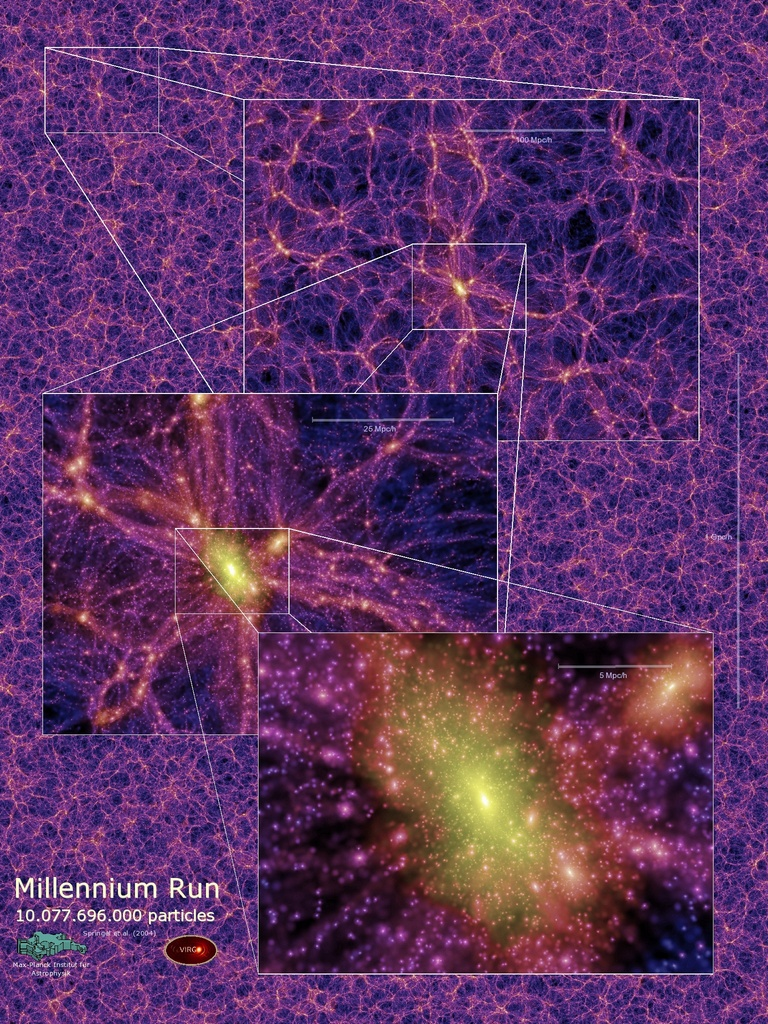
\includegraphics[width = 0.35\linewidth]{Millenium-Sim.jpg}
    \caption[Millennium Simulation Cosmic Web]{Se muestra el mapa de densidad de un corte de $15 Mpc/h$ en redshift $z=0$ de la \textit{Millennium Simulation}. Imagen obtenida de MPA}
    \label{fig:Millennium_Sim}
\end{figure}


%==================================================================================================
%==================================================================================================
%==================================================================================================
\subsubsection{Eagle Simulation}
El proyecto EAGLE (Evolution and Assembly of GaLaxies and their Environments)  es una colaboración de The Virgo Consortium, la cual es una simulación hidrodinámica de gran escala de un Universo de $\Lambda$CDM, el cual tenia como objetivo entender como las galaxias se forman y evolucionan. La mas grande de las simulaciones se realizo con  6.8 billones de partículas, en un volumen de 100 Mpc por lado, conteniendo al menos 10,000 galaxias del tamaño de la vía láctea, la cual tardo mas de un mes y medio de tiempo de computo y una de la mas grandes super-computadoras con 4000 núcleos de procesamiento usando una versión modificada del código de simulación GADGET-2 \cite{2015MNRAS.450.1937C, 2015MNRAS.446..521S}.

La simulación empieza en un Universo todavía muy uniforme (sin formación de estrellas o galaxias) usando parámetros motivados por las observaciones del satélite Plank \cite{ 2013ApJS..208...20B, 2020A&A...641A...1P}. Algunos de los parámetros cruciales de la simulación son la densidad de materia oscura, la cual es responsable de la formación de estructura de materia bariónica, así como la constante cosmológica, responsable de la expansión acelerada del Universo.
       
\begin{figure}[H]
    \centering
    \includegraphics[width = 0.45\linewidth]{Eagle-Sim.png}
    \caption[Eagle Simulation Cosmic Web]{Se muestra el mapa de densidad de la Eagle Simulation. Obtenida de \textit{The Eagle Project} }
    \label{fig:Eagle_Sim}
\end{figure}

%==================================================================================================
%==================================================================================================
%==================================================================================================

\section{La interacción dominante en las simulaciones}

Para estudiar el comportamiento de de un sistema de partículas, tenemos que simplificarlo la mas posible. Empezamos identificando la fuerza responsable del movimiento de las partículas, en este caso es la gravedad y en específico nos quedamos con la gravedad descrita por Newton \eqref{eq:Gravedad-Newton}. Por tanto, solo requerimos conocer las masas y las posiciones de las partículas.

\begin{equation}
    F = G \frac{m_1 m_2}{r^2}
    \label{eq:Gravedad-Newton}
\end{equation}

Pero como estamos tratando con sistema de $N$ partículas tenemos que considerar la contribución de fuerzas debida al resto de las partículas. Por el teorema de superposición podemos decir que
\begin{equation}
    F_{1} = F_{1,2} +F_{1,3} + \dots + F_{1,N} = \sum_{i=2}^{N} F_{1,i} 
    \label{eq:superposicion}
\end{equation}

Pero también podemos resolver el problema si trabajamos con el potencial
\begin{equation}
    \nabla \phi(\mathbf{r}) = \mathbf{F}
    \label{eq:potencial-gravitacional}
\end{equation}

%==================================================================================================
%==================================================================================================
%==================================================================================================
\section{Una razón práctica para las simulaciones}

Si consideramos las dimensiones de nuestra galaxia, podemos calcular el camino medio libre de una estrella antes de que colisione con otra estrella. En un sistema de partículas que se mueven en orbitas rectas, el camino medio libre es $\lambda = 1/(n\sigma)$ donde $n$ es la densidad numérica de partículas y $\sigma$ es la sección transversal de cada estrella. Asumiendo que todas las estrellas son como nuestro sol ($\sigma = \pi(2R_\odot)^2 $ donde $R_\odot = 6.96\times 10^{10}$ cm) y teniendo que en la galaxia hay aproximadamente $10^{11}$ estrellas distribuidas uniformemente sobre un disco de radio de $10 kpc$ y grosor de $1 kpc$, tenemos una densidad de numero de estrellas en el disco de $n=0.3pc^{-3}$. Por lo tanto el camino medio libre es de $\lambda = 1.5 \times 10^{33} cm = 5\times 10^{14}pc$. Ahora el tiempo entre colisiones es aproximadamente $\lambda / v$, donde $v$ es la velocidad aleatoria de una estrella en un lugar dado. Para $v=40km s^{-1}$ el intervalo entre colisiones es aproximadamente de $10^{19}$ años, $10^9$ veces mas antiguo que la edad de la galaxia \cite{Binney1988-rs}. Es evidente que las colisiones entre estrellas son lo suficientemente raras que no tienen importancia en la dinámica de las galaxias, por lo que para cualquier propósito, la dinámica de las estrellas en la galaxia se pueden aproximar a la de un conjunto de puntos masivos que no colisionan entre si, es decir un gas sin colisiones.

Como vemos que las colisiones entre estrellas de una galaxia son raras, podemos decir que a la escala del Universo sucede lo mismo. Por lo tanto, si queremos simular nuestro Universo, idealmente se debe resolver la ecuación de Boltzmann sin colisiones (CBE)

\begin{equation}
    \frac{d f}{d t} \equiv \frac{\partial f}{\partial t} + \mathbf{v}\frac{\partial f}{\partial \mathbf{x}} + \frac{\partial \Phi}{\partial \mathbf{r}} \frac{\partial f}{\partial \mathbf{v}}
    \label{eq:CBE}
\end{equation}

\noindent donde el potencial auto-consistente $\Phi$ es la solución a la ecuación de Poisson

\begin{equation}
    \nabla^2\Phi(\mathbf{r},t) = 4\pi G \int f(\mathbf{r},\mathbf{v},t)d\mathbf{v}
    \label{eq:PoissonSol}
\end{equation}

\noindent y $f(\mathbf{r},\mathbf{v},t)$ es la densidad de partículas en el espacio fase.

% En la práctica, no resolvemos CBE, sino que representamos el Universo como un sistema de N partículas, por lo tanto, se transforma en un problema de N-Cuerpos donde se siguen las ecuaciones de movimiento de Newton. Notemos que ahora es necesario introducir un radio de suavizado para pequeñas distancias con el objetivo de evitar que en el caso de una colisión de dos cuerpos, las partículas no salgan disparadas y para mantener el sistema sin colisiones. Según el número de partículas con el que se va a trabajar, va tener un efecto sobre como escoger el radio de suavizado.


% Pero lo que se realiza para simular nuestro Universo no es resolver CBE, si no que optamos por trabajar con un sistema de N-Cuerpos y ver 

% Es muy complicado resolver este sistema de ecuaciones. La solución a la que se a llegado es construir códigos para simulaciones de N-Cuerpos. Existen grandes cantidades de códigos para simulaciones de N-Cuerpos, pero se diferencian en como realizan los cálculos para el movimiento gravitacional. Además de que siempre están buscando la forma de hacer los simuladores mas rápidos y eficientes.

Seguir esta ruta presenta algunos retos tanto computacionales como físicos ya que debemos conocer bien la densidad en el espacio fase. Esta cantidad es prácticamente imposible de conocer para el Universo temprano, aunque se hacen algunos intentos por extrapolar posibles formas a partir de estructuras que vemos en el cielo actualmente (ver por ejemplo, [\cite[Binney]{Binney1988-rs} ], capítulo 7). 

La solución que se ha preferido es aproximar la dinámica mediante códigos de N-cuerpos, en los cuales se supone una interacción entre partículas dada por la interacción gravitacional clásica por pares de partículas en las cuales se agrega un radio de suavizado para evitar dividir por cero cuando se acercan mucho los cuerpos. 

Existen grandes cantidades de códigos para simulaciones de N-Cuerpos, pero se diferencian en como realizan los cálculos para el movimiento gravitacional. Además de que siempre están buscando la forma de hacer los simuladores mas rápidos y eficientes.
%==================================================================================================
%==================================================================================================
%==================================================================================================

\section{GADGET-4}
% Las simulaciones numéricas permiten el estudio detallado de formación de estructura y conecta a un Universo simple con alto corrimiento al rojo con uno con estructura compleja como la que se observa en la actualidad. 

Los código GADGET han sido de los mas utilizados en el estudió de formación de estructura y estudio de la materia oscura en las ultimas dos décadas. Han existido varias iteraciones de los códigos GADGET, siendo GADGET-4 la mas reciente y una renovación completa del simulador. 

La motivación detrás de la nueva versión de GADGET-4 fue construir un simulador con el cual se pudieran tener simulaciones mas grandes y con mayor precisión. Esto implica tener cálculos con gran poder estadístico y mayor resolución y para lograr esto, GADGET hace uso de métodos de paralelización avanzados. Pero debido a la necesidad de tener simulaciones cada vez mas grandes, se ha buscado mejorar escalabilidad del cogido GADGET \cite{2021MNRAS.506.2871S}.

Para esto se buscó quitar las limitaciones para grandes simulaciones, procurando que tenga un buen rendimiento en condiciones de alto rango dinámico en escalas de tiempo. También busca mejorar la precisión en los cálculos de fuerza gravitacional e hidrodinámica. Finalmente se buscó modernizar el código, quitando partes obsoletas y mejorando la legibilidad y la modularidad del código con el objetivo de que los usuarios puedan desarrollar con facilidad extensiones para el mismo. 

 
Una de las características que separa a GADGET de otros simuladores, es que es un código flexible multi-propósito que no restringe el tipo de simulaciones, sino que da prioridad a la flexibilidad  sobre la optimización para casos específicos. Para esto se implementaron un buen numero de nuevos métodos numéricos. También se introdujeron nuevas funcionalidades al código en la forma de la introducción de código para la búsqueda de grupos y sub-estructura (\textit{Friends of Friends} (FOF), SUBFIND) asi como un \textit{Merger Tree} que corre junto a la simulación. Se incluyo una nueva variación de un buscador de sub-estructura, SUBFIND-HBT, que usa la información de sub-halos del pasado en consideración, lo que permite una forma robusta y eficiente de seguir la sub-estructura en el tiempo incluso después de unirse a otro halo. GADGET también es capaz de generar sus condiciones iniciales ya sea usando la aproximación de Zeldovich o con la teoría de la perturbación lagrangiana de segundo orden (2PLT)\cite{2021MNRAS.506.2871S}.


\subsubsection{Cálculos de Gravedad de GADGET-4}

Tenemos un potencial $\Phi (\mathbf{x})$ producido por $N$ partículas con masas $m_j$ en coordenadas $x_j$ en el dominio con dimensiones $L_x \times L_y \times L_z$ que se replica periódicamente en las tres direcciones esta dado por:

\begin{equation}
    \Phi (\mathbf{x}) = - \sum_{j=1}^{N} \sum_{\mathbf{n}=-\infty}^{\infty}  \frac{ m_j }{ |\mathbf{x}_j - \mathbf{x} + \mathbf{q}_n| + |\epsilon ( \mathbf{x}_j - \mathbf{x} + \mathbf{q}_n)| }   - m_j\varphi_{\mathbf{n}}(\mathbf{x})
    \label{eq:Grav_Pot_1}
\end{equation}

\noindent donde $\mathbf{q_n}$ denota vectores de desplazamiento periódico dados por $\mathbf{q}_n$=($n_x$$L_x$,$ n_y$$L_y$,$n_z$$L_z$) y $\mathbf{n} = (n_x, n_y, n_z)$ son tripletes enteros y la suma sobre $\mathbf{n}$ se extiende sobre todo los tripletes. Se omitió la constante gravitacional $G$ por simplicidad. La contribución del potencial $\varphi_{\mathbf{n}}(\mathbf{x})$ es el de un cubo homogéneo de unidad de masa y extensión $L_x \times L_y \times L_z$ con un desplazamiento $\mathbf{q_n}$. Este termino se agrega para que la suma converja sobre un sistema periódico, de manera que efectivamente se establece neutralidad de carga gravitacional.

La función $\epsilon(r)$ describe a la ley de suavizado gravitacional. Debemos asumir que el suavizado tiene un rango finito, donde $\epsilon(r)=0$ para $r\geq r_0$ y donde $r_0$ es mas pequeño que la mitad de la dimensión mas pequeña de la caja. En GADGET se ha adoptado un potencial donde el potencial de una partícula puntual se remplaza por un potencial con una distribución de masa suave con bordes en $h=2.8\epsilon_0$, donde $\epsilon_0$ es el radio de suavizado. La ley de suavizado esta dada por:

\begin{equation}
    \epsilon(r;\epsilon_0) = - \frac{2.8\epsilon_0}{W_2(r/2.8\epsilon_0)} -r
    \label{eq:Ley-Suavizado}
\end{equation}

Ahora definamos $\mathbf{q}^*_j(x)$ como el desplazamiento periódico que minimiza la distancia de $\mathbf{x}_j+\mathbf{q}_n$ a $x$ (es decir selecciona la ubicación de la partícula $j$ imagen periódica mas cercana a la posición $\mathbf{x}$), podemos escribir el potencial como:
% Esencialmente para resolver el sistema de N-cuerpos, el potencial gravitacional que se usa para calcular el movimiento de las N partículas es el siguiente:

\begin{align}
    \Phi (\textbf{x}) = &- \sum_{j=1}^{N} \frac{m_j}{|\textbf{x}_j-\textbf{x}+\textbf{q}^*_j| + |\epsilon(\textbf{x}_j-\textbf{x}+\textbf{q}^*_j)|} \nonumber \\
    &+ \sum_{j=1}^{N} m_j \psi (\textbf{x}_j-\textbf{x}+\textbf{q}^*_j) \label{eq:Pot}
\end{align}

\noindent donde la primera parte es el potencial gravitacional de newton con una corrección para considerar el radio de suavizado y el segundo termino en potencial se introduce como una corrección para el suavizado de imágenes distantes. Este es el potencial que GADGET-4 usa como base para los cálculos de gravedad, pero como GADGET es un simulador diseñado para abarcar una amplia gama de necesidades, sus desarrolladores implementaron diversos algoritmos para la forma en la que se realizaron los cálculos.


\subsubsection{Buscador de grupos y sub-halos}

Las simulaciones cosmológicas son una herramienta util para simular el movimiento de cuerpos en nuestro Universo, pero ocupamos mas herramientas para poder describir las propiedades del Universo. En GADGET-4 se han implementado una diversa cantidad de herramientas con las que podemos estudiar nuestras simulaciones y muchas de estas corren junto a la simulación, lo que permite tener mejores resultados. Algunas de las herramientas que tiene GADGET son buscador de grupos y sub-halos, construcción de arboles de fusión, conos de luz, estimación del espectro de potencia y generación de condiciones iniciales. 

La herramienta de nuestro interés fue el buscador de grupos y sub-halos. GADGET tiene tres implementaciones distintas. Se implementó un \textit{Friends of Friends} (FOF), un algoritmo SUBFIND para buscar sub-estructura ligada gravitacionalmente y nueva variante SUBFIND-HBT el cual usa información pasada de miembros del grupos para ver la evolución de los grupos y sub-halos.

\subsubsection{ Friends of Friends (\textbf{FOF}) }
El algoritmo de FOF organiza los halos en una lista de enlaces. Este empieza poniendo todas las partículas en su propio grupo, luego el se busca todos los pares de partículas con una distancia menor a longitud de enlace $l$. El valor mas común de $l$ es $0.2$ veces la distancia media entre partícula. De esta manera los halos están ligados por contornos de densidad que aproximan sobre-densidades. Cada par que se encuentra con una distancia suficiente pequeña, provoca que los grupos a los que pertenecen se unan.La implementación de GADGET se ha reportado tener mayores velocidades comparados con otras implementaciones en la literatura \cite{2021MNRAS.506.2871S}.

\subsubsection{SUBFIND}
En la búsqueda de estructuras de materia oscura, el buscador FOF se puede combinar con el algoritmo SUBFIND. La idea es checar si los halos encontrados son estructuras ligadas gravitacionalmente. Primero se busca el campo de densidad, donde se busca picos de densidad aislados. De ahi se buscan los puntos sillas que conectan dos picos de densidad. El pico pequeño se registra como un candidato de sub-estructura, el cual se somete a un procedimiento con el cual se verifica que se encuentra ligado gravitacionalmente. 

En la implementación que se realizó en GADGET-4, para la selección de cuales picos son sub-estructura y cuales solo están en el fondo (no forman parte de la sub-estructura), se puede tomar en cuenta la historia de las partículas sobre a cuales halos formo parte en el pasado. Esto lo puede hacer mientras se evoluciona el sistema de la simulación tomando en cuenta a que halos han pertenecido y la suma acumulada del tamaño del halo, mientras que en el si se realiza al terminar la simulación esta información se recolecta de los snapshots en orden temporal. El pico con la mayor suma se identifica como un pico del fondo (no es necesariamente el pico con la mayor cantidad de partículas).

\subsubsection{SUBFIND-HBT}
Hemos visto dos herramientas que nos permiten identificar estructuras, cada una con una aproximación diferente para determinar la pertenencia de las partículas a estructura. Ahora veremos la última implementación de buscador de estructura que tiene GADGET-4. SUBFIND identifica estructura ligada gravitacionalmente en el espacio coordenado en un solo corte temporal. Este método tiende a ser demandante computacionalmente y tiende a tener problemas identificando toda la materia que contiene la sub-estructura, especialmente cerca del pericentro del subhalo que orbita un halo mas grande. 

Este método tiende a ser muy rápido ya que suele omitir el paso donde verifican si las partículas se encuentran ligadas gravitacionalmente, lo que hace que las estructuras identificadas tengan una naturaleza física no definida seguramente. Una alternativa es depender de información pasada para la identificación de halos. Si tenemos un conjunto de partículas que se encuentran ligadas gravitacionalmente y se clasifica como una sub-estructura de un sistema mas grande, se puede checar continuamente si las partículas siguen ligadas. Esto asume que las estructuras solo pueden perder partículas y que no crecen en masa en una manera apreciable cuando se encuentra en órbita de un sistema mas grande. Este algoritmo se le conoce como \textit{Hierarchically Bound Tracing}(HBT).

GADGET-4 implemento una variante de HBT+. En la practica, este algoritmo puede reemplazar a SUBFIND teniendo la misma estructura de salida, a este enfoque SUBFIND-HBT. Funciona solamente con los snapshots en secuencia procesados en orden temporal. El método primeramente encuentra nuevos grupos FOF. Después se identifican candidatos para sub-estructura en cada grupo FOF basados en su pasadas afiliaciones de sub-estructuras. Los candidatos mas grandes encontrados se descartan por el momento, debido a que el procedimiento lo identifica como el halo del fondo del grupo, el cual puede crecer en masa. El resto de los candidatos se someten a un proceso para identificar si las partículas siguen ligas a la sub-estructura usando sus coordenadas en el espacio fase. Este método es significativamente mas simple y barato computacionalmente ya que no se necesita calcular el campo de densidad y por tanto no hay necesidad de procesar el calculo de los puntos sillas. La gran ventaja es que capaz de recuperar la masa total de todas las sub-estructuras, incluso de las que están cerca del pericentro en su orbita \cite{2021MNRAS.506.2871S}.
%%
%% cap3.tex
%% 
%% Made by Carlos Calcaneo Roldan
%% Login   <calcaneo@jogrant>
%% 
%% Started on  Mon Jul 22 15:03:25 2019 Carlos Calcaneo Roldan
%% Last update Time-stamp: <2020-jul-29.miércoles 19:05:05 ()>
%%
%%%%%%%%EL TExto Comienza abajo de aquí! 
\chapter{Halos de Materia Oscura}
\setcounter{equation}{0}

\noindent Con la intención de conocer y diferenciar diferentes cosmologías, en nuestro estudio de los halos de materia oscura, optamos por realizar fue una variedad de simulaciones de materia oscura. Desde simulaciones con cosmologías de Universos planos ($\Omega = 1$), asi como cosmologías  de universos con densidades sub-criticas ($\Omega < 1$) y super-criticas ($\Omega > 1$). Las simulaciones que realizamos empezaron en un corrimiento al rojo de $z=63$ hasta un $z=0$.

%====================================================================================================================
%======================================  COSMO PLANA  ===============================================================
%====================================================================================================================
\section[Cosmología Plana \texorpdfstring{$\Omega = 1$}{Omega = 1}]{Cosmología Plana \texorpdfstring{$\Omega = 1$}{Omega = 1}}

\noindent Comenzaremos con un estudio de las cosmologías planas (aquellas donde las densidades sean $\Omega = 1$). Estudiaremos 3 cosmologías planas, empezando con las que tiene las densidades mas aceptadas de nuestro Universo ($\Omega_\lambda = 0.691$, $\Omega_0 = 0.309$  \cite{2020A&A...641A...1P}). Luego pasaremos nuestra atención a estudiar los efectos que hay con las densidades invertidas ($\Omega_\lambda = 0.309$, $\Omega_0 = 0.691$) y para terminar con las cosmologías planas veremos los efectos en un Universo con densidades iguales ($\Omega_\lambda = 0.5$, $\Omega_0 = 0.5$).

%====================================================================================================================
%======================================  CANON RUN  =================================================================
%====================================================================================================================
\subsection{Universo con cosmología  \texorpdfstring{$\Omega_\lambda = 0.691$, $\Omega_0 = 0.309$ }{Omega lambda = 0.691, Omega 0 = 0.309}  }

 En la evolución de este Universo, la materia comienza a agruparse lentamente en lo que llamamos halos. En un principio la materia parece una nube difusa sin estructuras internas, después de un tiempo en el que se esta agrumando, pequeñas estructuras de materia se empiezan a formar. Las primeras estructuras son pocas como se aprecia en la figura \ref{fig:Canon_TotalHalos}. Las estructuras tardan tiempo en aparecer y eventualmente hay un aumento acelerado en la cantidad halos que se forman y mas hacia al presente vemos un pico donde empiezan a disminuir el total de halos.

\begin{figure}[H]
    \centering
    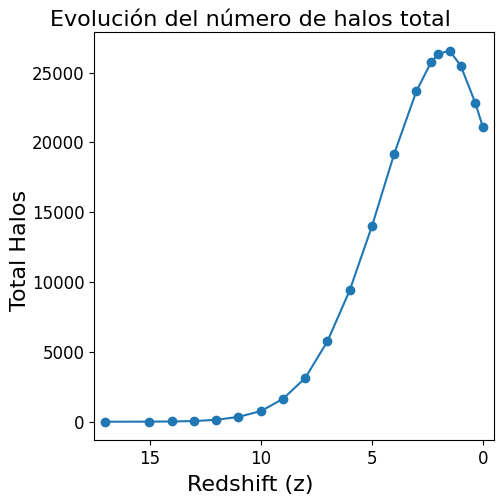
\includegraphics[scale = 0.5]{RunCanonica/TotalHalos_RunCanonica.png}
    \caption[Evolución del número de halos en un Universo $\Omega_\lambda = 0.691 $, $\Omega_0 = 0.309$]{\footnotesize Se muestra el numero de halos según el redshift y podemos observar como evoluciona el Universo en una cosmología $\Omega_\lambda = 0.691 $ y $\Omega_0 = 0.309$.}
    \label{fig:Canon_TotalHalos}
\end{figure}

La distribución de la masa para esta cosmología se observa en las figuras \ref{fig:Canon-MassDistSep} y \ref{fig:Canon-MassDist}. Los rangos de la masa se encuentran entre las $10^{10.11}M_\odot$ a $10^{14.32}M_\odot$ a lo largo de de la evolución del sistema. Las primeras estructuras, las que tienen $z$ altos, tenían masas menores a las $10^{11}M_\odot$ y las estructuras en $z$ pequeños la mayor parte de los halos tenían masas entre $10^{10.5}M_\odot$ y $10^{11.5}M_\odot$ con estructuras que alcanzan $10^{14.32}M_\odot$. Mientras, la figura \ref{fig:Canon-MassStats} nos muestra el comportamiento medio durante la evolución donde observamos que la masa media incrementa desde $10^{10.41}M_\odot$ con una desviación de $10^{0.11}M_\odot$ en $z=15$ hasta $10^{10.75}M_\odot$ con una desviación de $10^{0.49}M_\odot$ en $z=0$.

\begin{figure}[H]
    \centering
    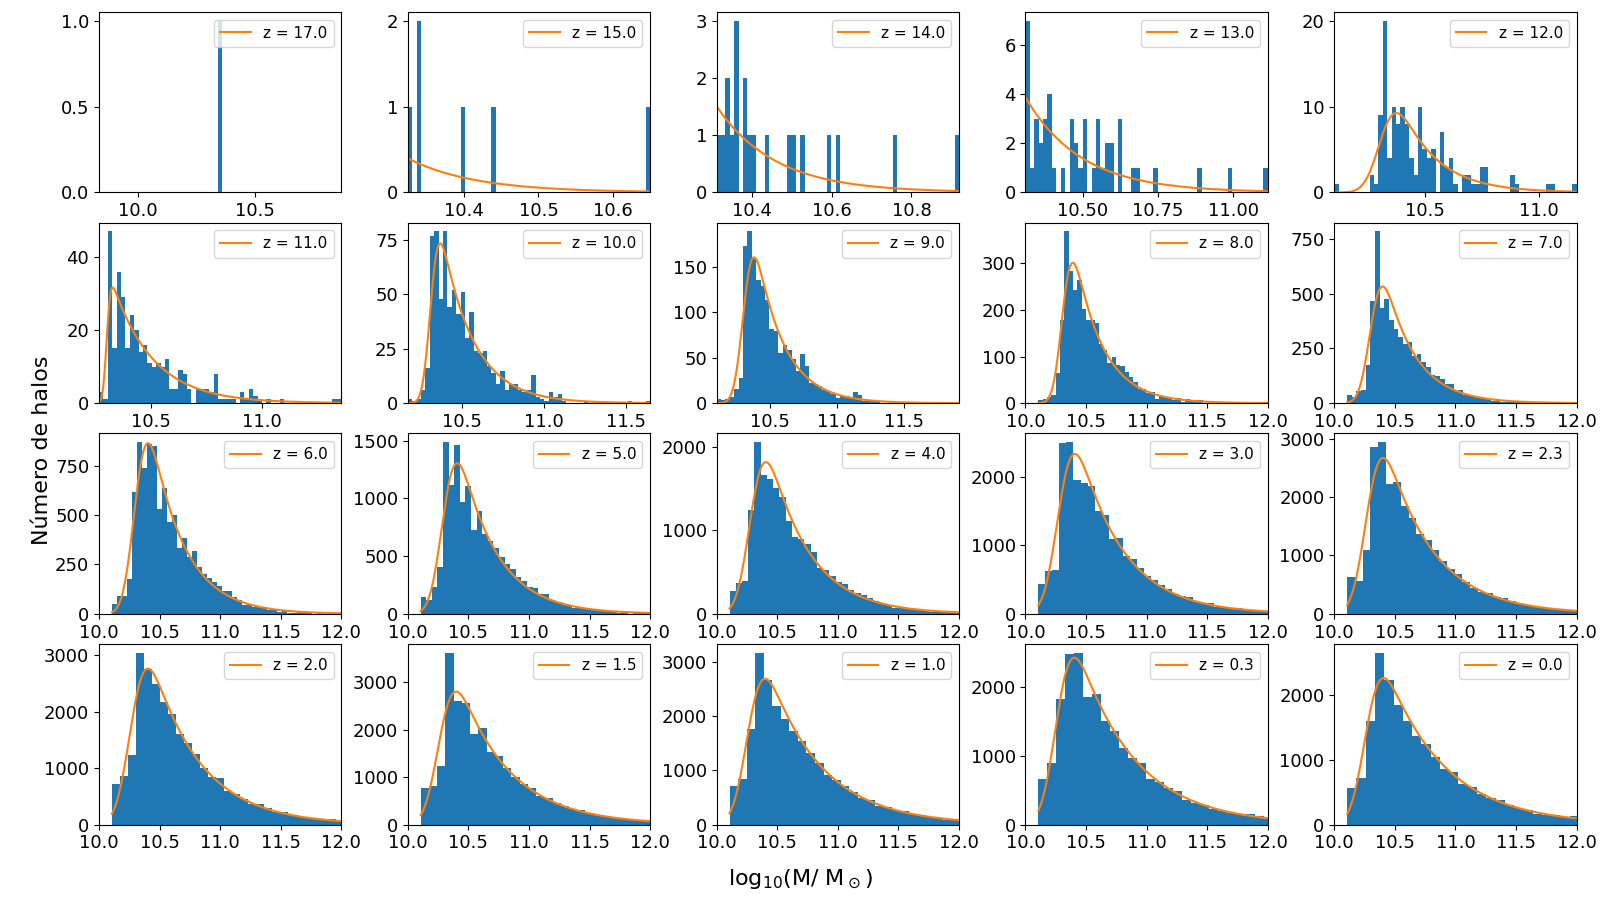
\includegraphics[width = 0.8\linewidth]{RunCanonica/Mass_Dist_RunCanonicaSep.png}
    \caption[Distribución de masa]{\footnotesize Tenemos la cantidad de halos en diferentes rangos de masa. Se muestran la distribución de la masa conforme evoluciona el Universo en una cosmología $\Omega_\lambda = 0.691 $ y $\Omega_0 = 0.309$. Se tienen las distribuciones en los diferentes redshifts empezando en $z=17$ en la parte superior izquierda y terminado en $z=0$ en la parte inferior derecha. Se observa como aumentan la cantidad de halos cada vez mas masivos.}
    \label{fig:Canon-MassDistSep}
\end{figure}

\begin{figure}[H]
    \centering
    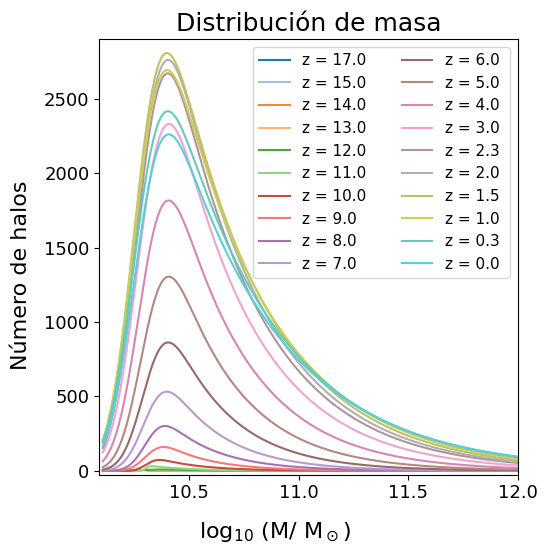
\includegraphics[width = 0.5\linewidth]{RunCanonica/Mass_Dist_RunCanonica.png}
    \caption[Comparación de distribución de masa]{\footnotesize Tenemos la cantidad de halos en los diferentes rangos de masa. Comparamos de las distribuciones de masa durante la evolución del Universo $\Omega_\lambda = 0.691 $, $\Omega_0 = 0.309$. Se muestra la cantidad de halos en un rango de masas. Se observa como crece la cantidad de halos de materia oscura, asi como el tamaño de estos.}
    \label{fig:Canon-MassDist}
\end{figure}

\begin{figure}[H]
    \centering
    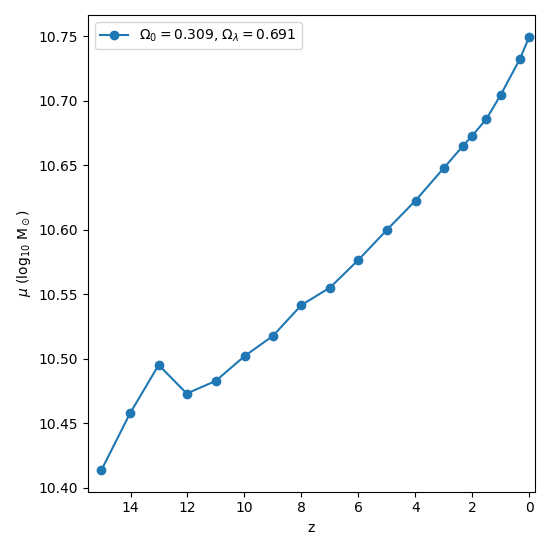
\includegraphics[width = 0.4\linewidth]{RunCanonica/MassMean_RunCanonica.png}
    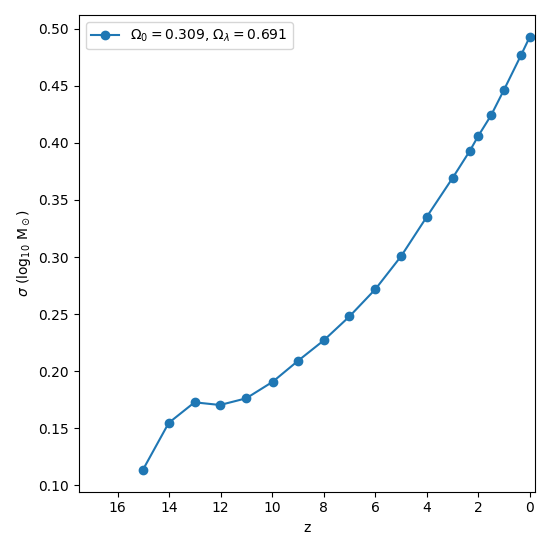
\includegraphics[width = 0.4\linewidth]{RunCanonica/MassStd_RunCanonica.png}
    \caption[Media y desviación estándar de la distribución de masa]{\footnotesize En la izquierda se muestra la masa media de los halos de materia oscura y se observa como cambia durante la evolución del Universo. En la derecha se muestra la desviación estándar de la masa, la cual nos muestra la variedad que hay de los halos de materia oscura, desde un z = 17 hasta un z = 0.}
    \label{fig:Canon-MassStats}
\end{figure}

En las figuras \ref{fig:Canon-HalfMassRadDistSep} y \ref{fig:Canon-HalfMassRadDist} podemos ver el radio que contiene la mitad de la masa de los halos a lo largo de la evolución del Universo. Vemos que los radios se encuentran entre los $10^{0.24}$kpc y $10^{2.69}$kpc donde los primeros halos tienen radios entre los $10^{0.24}$kpc y los $10^{1.01}$ y las estructuras mas recientes tienen la mayor parte de los halos en el rango de $10^{1.25}$kpc y los $10^{1.7}$kpc con halos que alcanzan hasta los $10^{2.69}kpc$. En la figura \ref{fig:Canon-HalfMassRadStats} vemos el crecimiento del radio medio desde $10^{0.44}$kpc con una desviación de $10^{0.06}$kpc en $z=15$ hasta un radio de $10^{1.47}$kpc con una desviación de $10^{0.19}$kpc en $z=0$.

\begin{figure}[H]
    \centering
    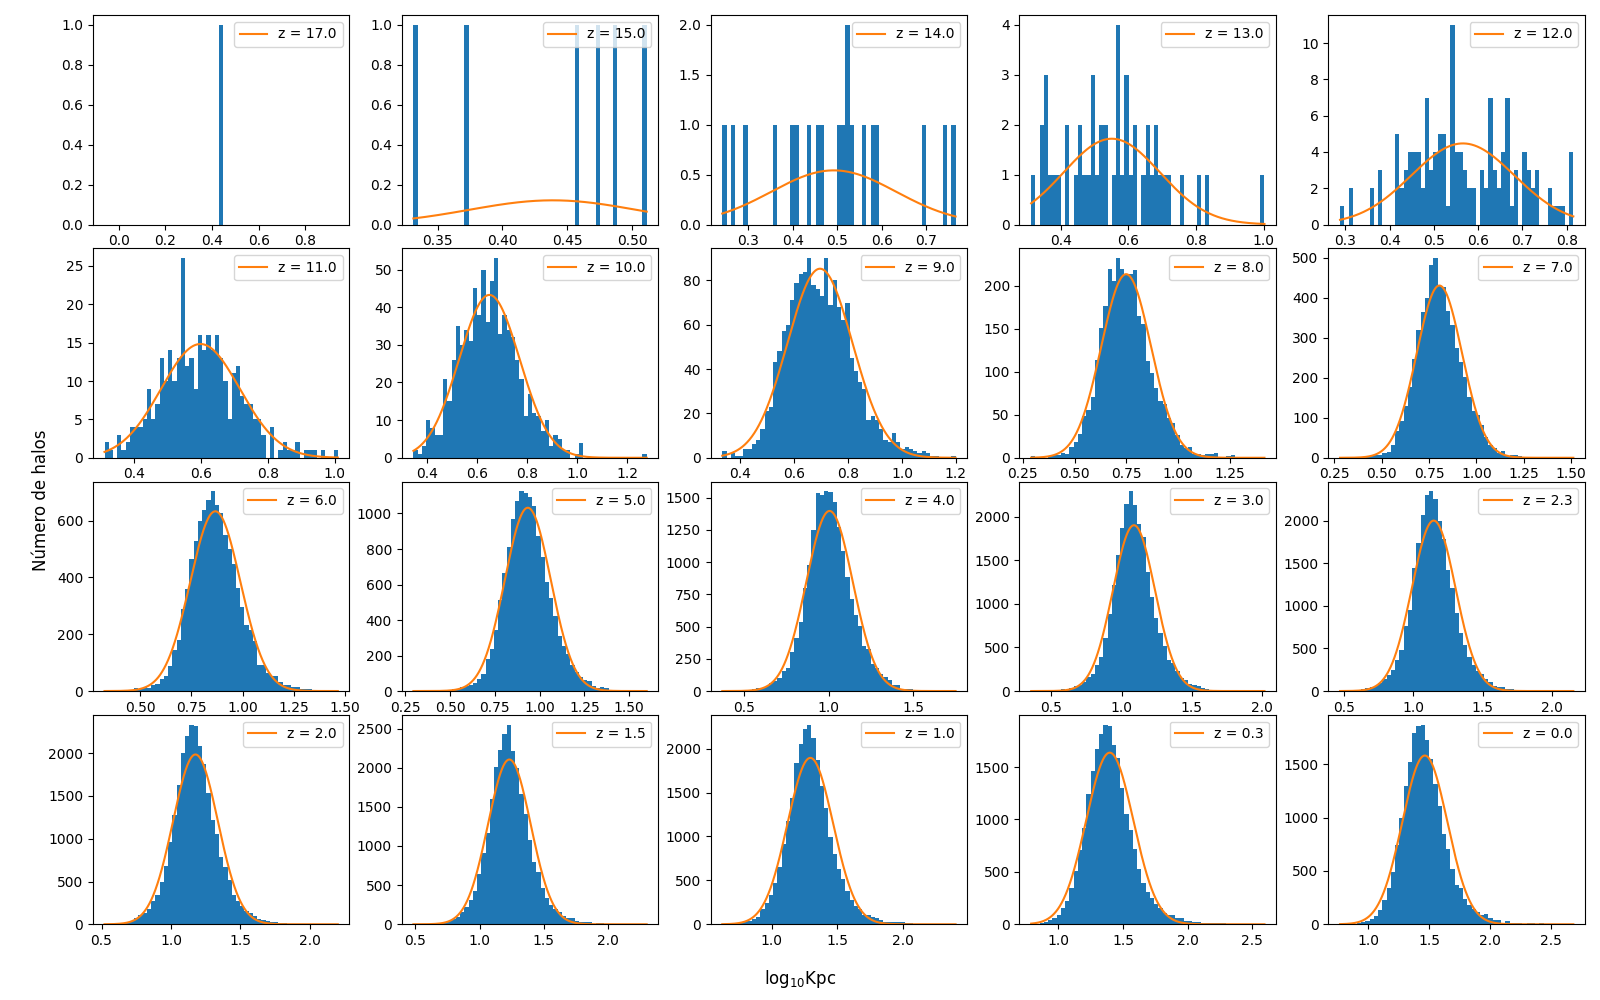
\includegraphics[width = 0.75\linewidth]{RunCanonica/HalfMassRad_Dist_RunCanonicaSep.png}
    \caption[Radio que contiene la mitad de la masa]{\footnotesize Se muestra la cantidad de halos que tiene el radio que contiene la mitad de la masa conforme evoluciona el Universo en una cosmología $\Omega_\lambda = 0.691 $ y $\Omega_0 = 0.309$. Se tienen las distribuciones en los diferentes redshifts empezando en $z=17$ en la parte superior izquierda y terminado en $z=0$ en la parte inferior derecha.}
    \label{fig:Canon-HalfMassRadDistSep}
\end{figure}

\begin{figure}[H]
    \centering
    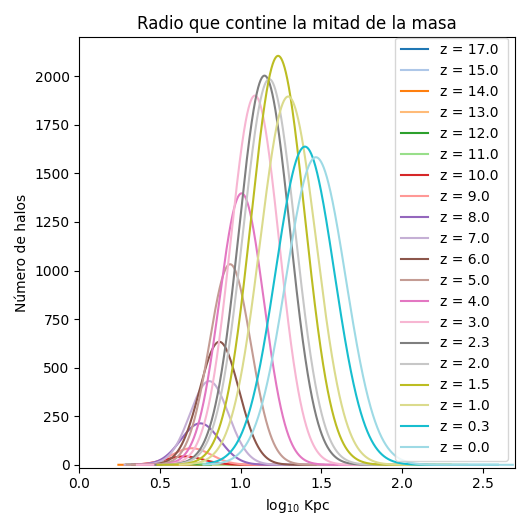
\includegraphics[width = 0.5\linewidth]{RunCanonica/HalfMassRad_Dist_RunCanonica.png}
    \caption[Distribución del radio que contiene la mitad de la masa]{\footnotesize Mostramos la cantidad de halos de materia oscura que tienen un radio que contiene la mitad de la masa en un Universo $\Omega_\lambda = 0.691 $, $\Omega_0 = 0.309$ desde un $z=17$ hasta un $z=0$.}
    \label{fig:Canon-HalfMassRadDist}
\end{figure}

\begin{figure}[H]
    \centering
    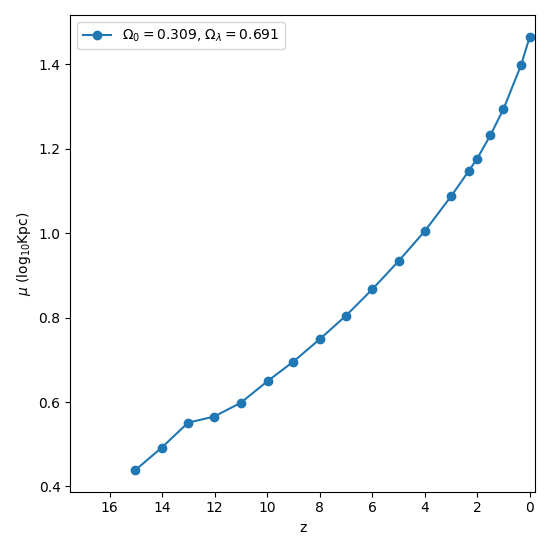
\includegraphics[width = 0.4\linewidth]{RunCanonica/HalfMassRad_Mean_RunCanonica.png}
    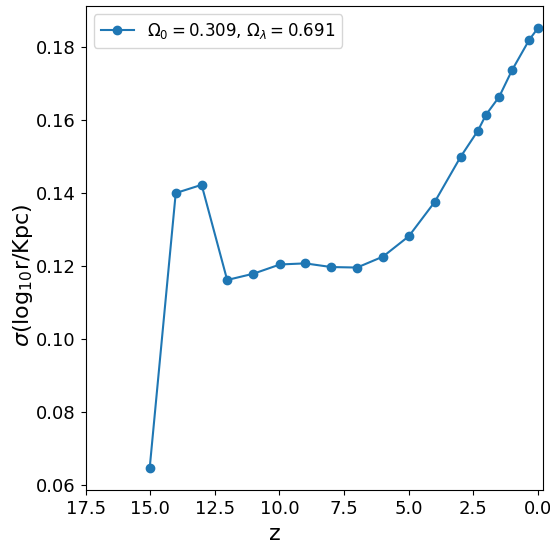
\includegraphics[width = 0.4\linewidth]{RunCanonica/HalfMassRad_Std_RunCanonica.png}
    \caption[Media y desviación estándar del radio de la mitad de la masa]{\footnotesize En la izquierda mostramos la media del radio que contiene la mitad de la masa de los halos de materia oscura y en la derecha se muestra su desviación estándar a lo largo de la evolución del Universo, desde un $z=17$ hasta un $z=0$.}
    \label{fig:Canon-HalfMassRadStats}
\end{figure}

Otra medida que utilizamos para dar una idea en el tamaño que tienen los halos es usando el radio donde tenemos la mayor velocidad radial. En las figuras \ref{fig:Canon-VMaxRadDistSep} y \ref{fig:Canon-VMaxRadDist} observamos que a lo largo de la evolución de las estructuras, tenemos halos con radios que van desde los $0.72$kpc hasta los $452.28$kpc. Vemos que la gran mayoría de los halos son halos con tamaños menores a $50$kpc con halos que alcanzan hasta los $452.28$kpc mas al presente y menores a $10$kpc con estructuras que alcanzan $9.83$kpc en los redshifts mas altos. En la figura \ref{fig:Canon-VMaxRadStats} vemos que la media va desde los $2.45$kpc con una desviación de $0.88$kpc en $z=15$ hasta $27.60$kpc con una desviación de $15.69$kpc en $z=0$.

\begin{figure}[H]
    \centering
    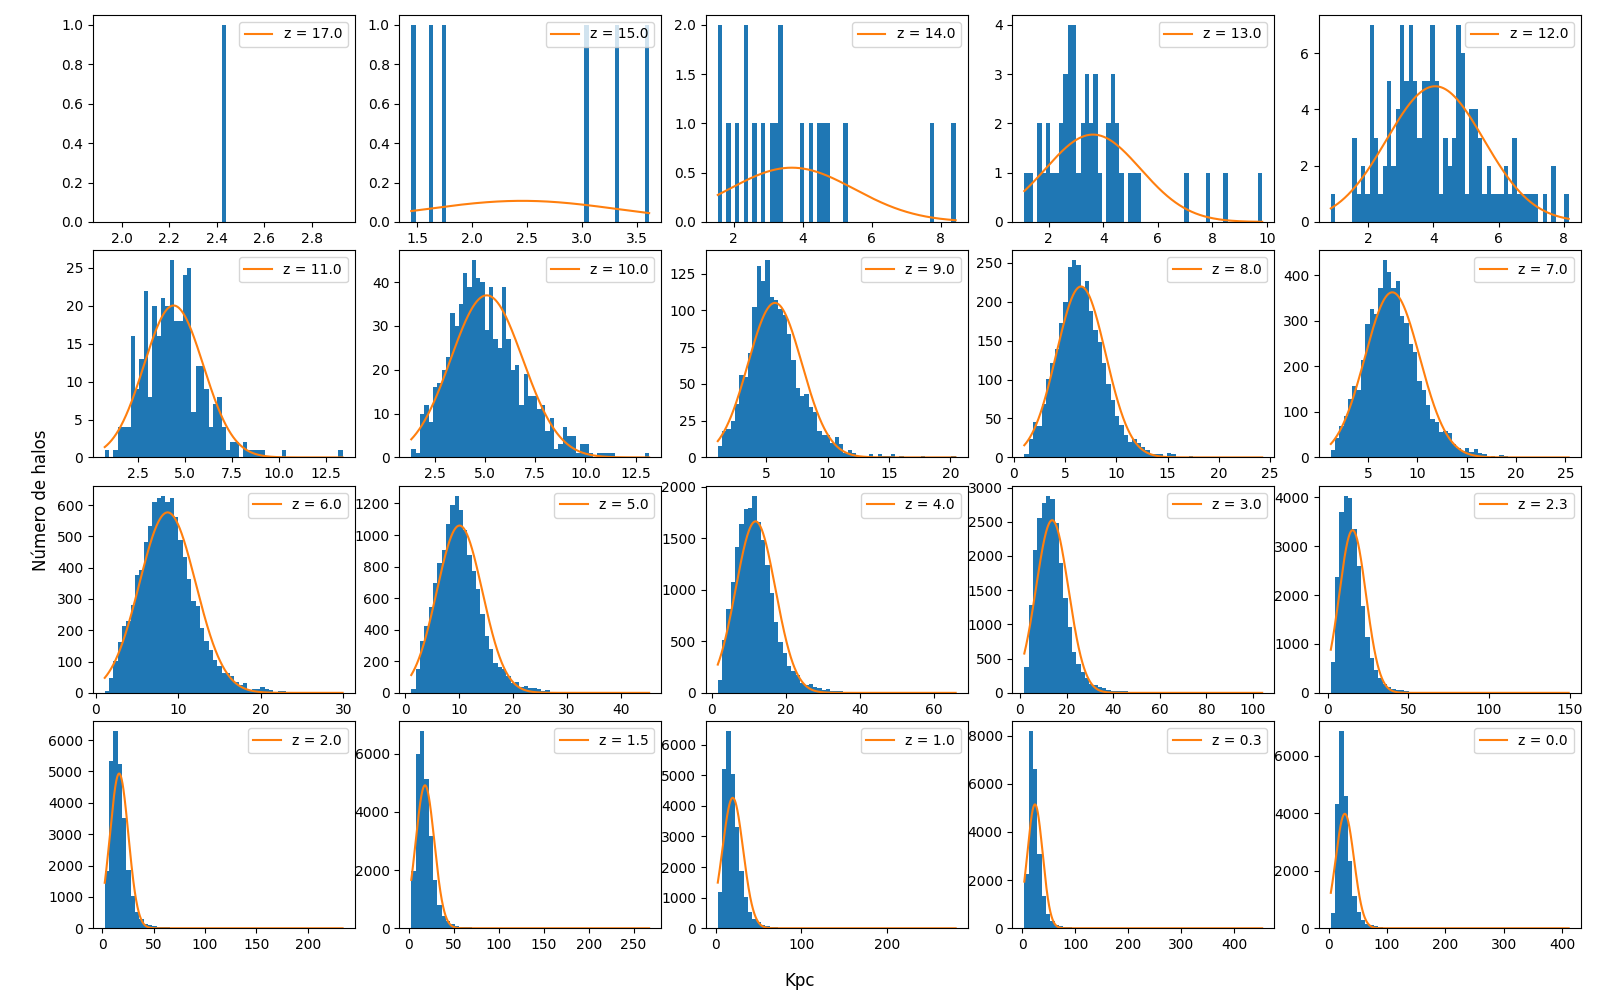
\includegraphics[width = 0.75\linewidth]{RunCanonica/VMaxRad_Dist_RunCanonicaSep.png}
    \caption[Radio donde se alcanza la velocidad máxima radial]{\footnotesize Se muestra el radio donde se alcanza la velocidad máxima radial conforme evoluciona el Universo en una cosmología $\Omega_\lambda = 0.691 $ y $\Omega_0 = 0.309$. Se tienen las distribuciones en los diferentes redshifts empezando en $z=17$ en la parte superior izquierda y terminado en $z=0$ en la parte inferior derecha.}
    \label{fig:Canon-VMaxRadDistSep}
\end{figure}

\begin{figure}[H]
    \centering
    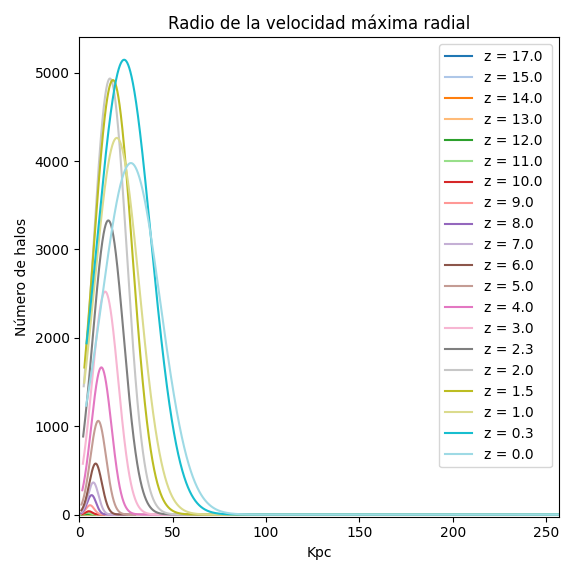
\includegraphics[width = 0.5\linewidth]{RunCanonica/VMaxRad_Dist_RunCanonica.png}
    \caption[Distribución del radio donde se alcanza la velocidad máxima radial]{\footnotesize Se muestra la cantidad de halos de materia oscura con el radio donde se alcanza la velocidad máxima radial en un Universo $\Omega_\lambda = 0.691 $, $\Omega_0 = 0.309$.}
    \label{fig:Canon-VMaxRadDist}
\end{figure}

\begin{figure}[H]
    \centering
    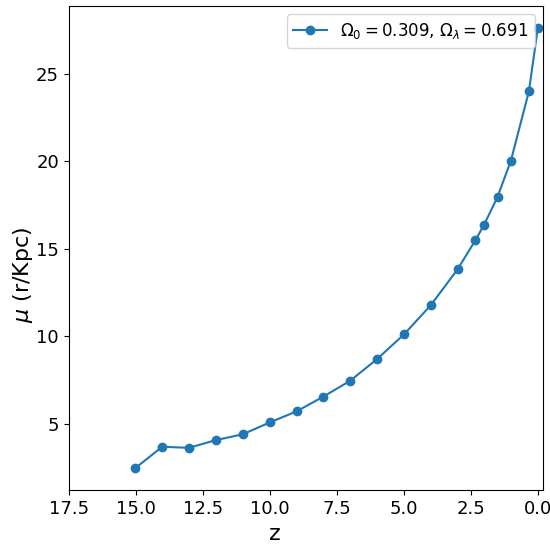
\includegraphics[width = 0.4\linewidth]{RunCanonica/VMaxRad_Mean_RunCanonica.png}
    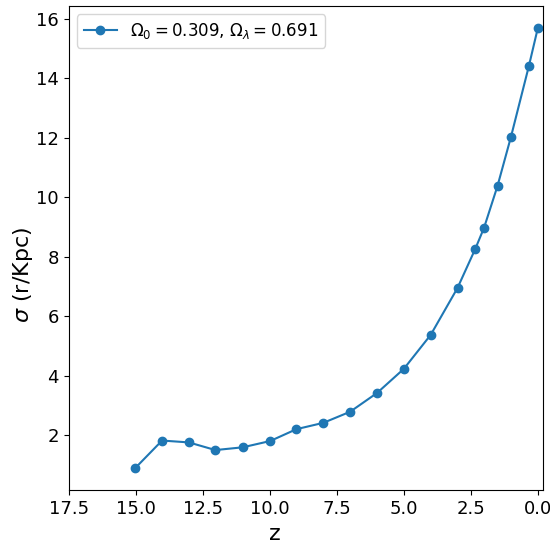
\includegraphics[width = 0.4\linewidth]{RunCanonica/VMaxRad_Std_RunCanonica.png}
    \caption[Media y desviación estándar del Radio donde se alcanza la velocidad máxima radial]{\footnotesize En la izquierda mostramos la media del radio donde se alcanza la velocidad máxima radial de los halos de materia oscura y en la derecha se muestra su desviación estándar a lo largo de la evolución del Universo, desde un $z=17$ hasta un $z=0$.}
    \label{fig:Canon-VMaxRadStats}
\end{figure}

Pasando a las velocidades, empezando con la velocidad circular máxima. Podemos apreciar que las velocidades circulares van de los rangos de los $22.82$km/s hasta los $1001.91$km/s donde vemos la gran mayoría de los halos en los rangos de $100$km/s y $175$km/s para los $z$ altos y entre los $50$km/s y $175$km/s mas al presente, como se muestra en las figuras \ref{fig:Canon-VelMaxDistSep} y \ref{fig:Canon-VelMaxDist}. Lo que podemos ver en la figura \ref{fig:Canon-VelMaxStats} es que la velocidad  media disminuye rápidamente desde $150.13$km/s con una desviación de $26.76$km/s en $z=15$ hasta que alcanza $74.77$km/s con una desviación de $33.90$km/s en $z=0$.

% Pasando a las velocidades, empezando con la velocidad circular máxima, en las figuras \ref{fig:VelMaxDistSep} y \ref{fig:VelMaxDist} podemos ver que un pequeña parte de los halos tienen velocidades mayores a $200$ km/s a lo largo de la evolución del Universo. La mayor parte tienen velocidades entre $40$ y $150$km/s. Algo que se observa en la figura \ref{fig:VelMaxStats} es que la velocidad media disminuye conforme avanza el tiempo, pero también vemos un aumento en la diversidad de velocidades que hay. La media en un universo temprano se encontraba entre los $130$ y $150$ km/s con variaciones entre $10$ y $30$ km/s. En el presente tenemos una media de $74.7$ km/s con desviación de $33.9$ km/s. 

\begin{figure}[H]
    \centering
    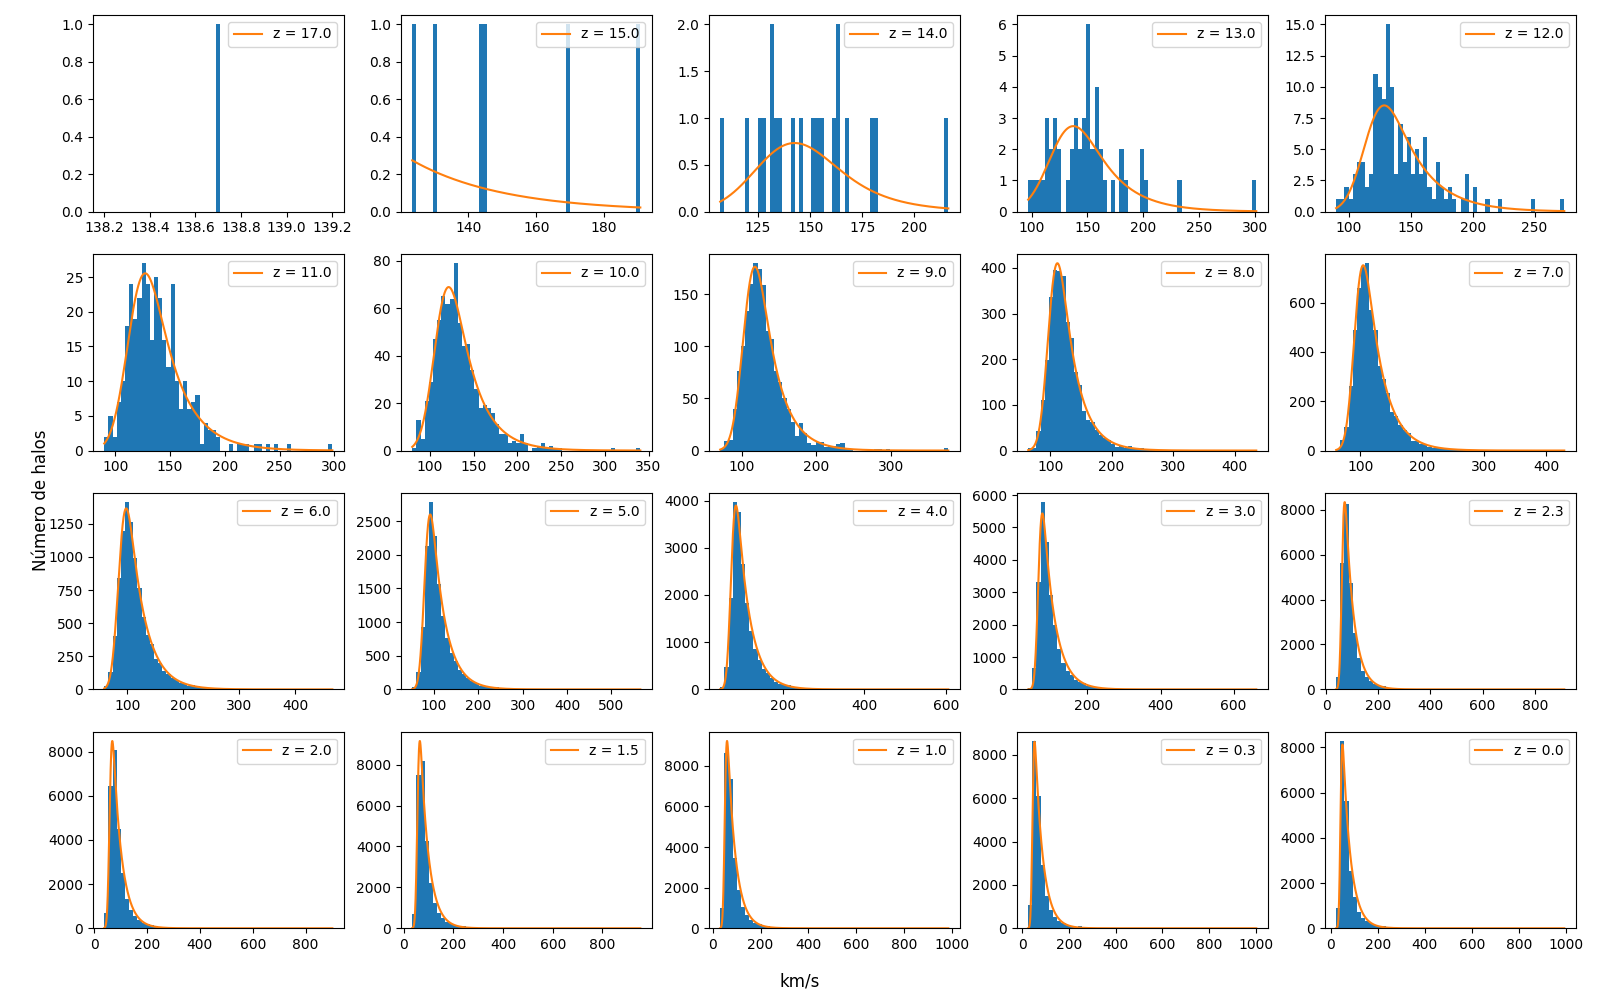
\includegraphics[width = 0.75\linewidth]{RunCanonica/VelMax_Dist_RunCanonicaSep.png}
    \caption[Velocidad circular máxima]{\footnotesize Se muestra la velocidad circular máxima conforme evoluciona el Universo en una cosmología $\Omega_\lambda = 0.691 $ y $\Omega_0 = 0.309$. Se tienen las distribuciones en los diferentes redshifts empezando en $z=17$ en la parte superior izquierda y terminado en $z=0$ en la parte inferior derecha.}
    \label{fig:Canon-VelMaxDistSep}
\end{figure}

\begin{figure}[H]
    \centering
    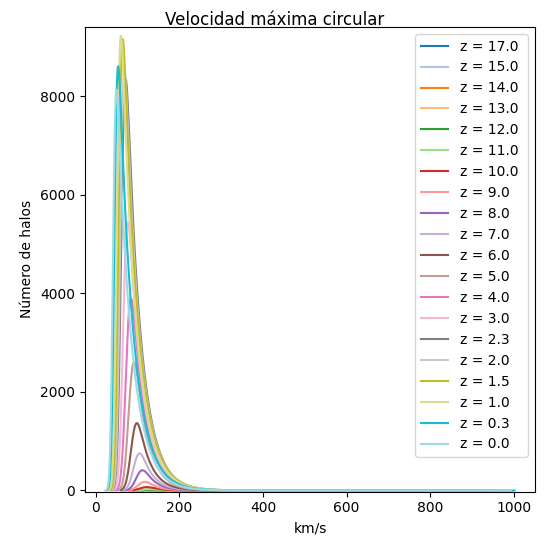
\includegraphics[width = 0.5\linewidth]{RunCanonica/VelMax_Dist_RunCanonica.png}
    \caption[Distribución de la velocidad circular máxima]{\footnotesize Mostramos la cantidad de halos de materia oscura en los diferentes rangos de velocidad circular máxima en un Universo $\Omega_\lambda = 0.691 $, $\Omega_0 = 0.309$.}
    \label{fig:Canon-VelMaxDist}
\end{figure}

\begin{figure}[H]
    \centering
    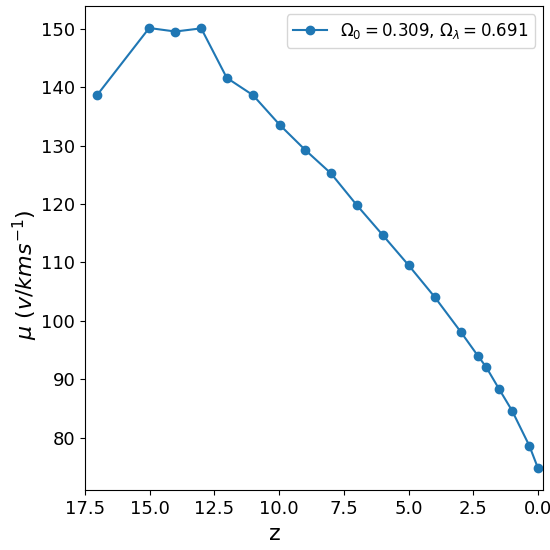
\includegraphics[width = 0.4\linewidth]{RunCanonica/VelMax_Mean_RunCanonica.png}
    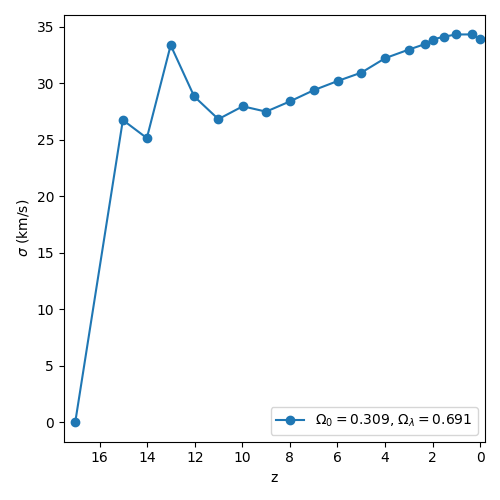
\includegraphics[width = 0.4\linewidth]{RunCanonica/VelMax_Std_RunCanonica.png}
    \caption[Media y desviación estándar de la velocidad circular máxima]{\footnotesize En la izquierda mostramos la media de la velocidad circular máxima de los halos de materia oscura y en la derecha se muestra su desviación estándar a lo largo de la evolución del Universo.}
    \label{fig:Canon-VelMaxStats}
\end{figure}

Ahora hablemos de la dispersion de las velocidades de los halos de materia oscura. La dispersión de velocidades de estos halos esta en los rangos de $12.78$km/s a los $619.79$km/s a lo largo de la evolución de los halos. Vemos en las figuras \ref{fig:Canon-VelDispDistSep} y \ref{fig:Canon-VelDispDist} que en los $z$ altos vemos que que la mayor parte de los halos se encuentran en el rango de los $60$km/s a los $100$km/s con picos en los $183.94$km/s, mientras que en los $z$ bajos vemos los rango que van de $50$km/s y $80$km/s con los picos entre los $355.62$km/s y $619.79$km/s. En la figura \ref{fig:Canon-VelDispStats} observamos que la dispersión de velocidades media disminuye desde los $85.25$km/s con una desviación de $13.09$km/s en $z=15$ a $37.08$km/s con una desviación de $18.69$km/s en $z=0$.

% Para terminar de hablar de la dinámica interna del halo, las figuras \ref{fig:VelDispDistSep} \ref{fig:VelDispDist} nos muestran las distribuciones de la dispersión de velocidades. Observamos un comportamiento similar a la velocidad máxima circular, donde vemos casos pocos situaciones con dispersiones mayores de $150$ km/s. Ademas, si observamos la figura \ref{fig:VelDispStats}, podemos apreciar una disminución en la dispersion de velocidades media similar a la media de la velocidad circular máxima. En este caso vemos que la dispersión de velocidades media varia desde $86.5$ km/s en el pasado, hasta $37$ km/s en el presente. 

\begin{figure}[H]
    \centering
    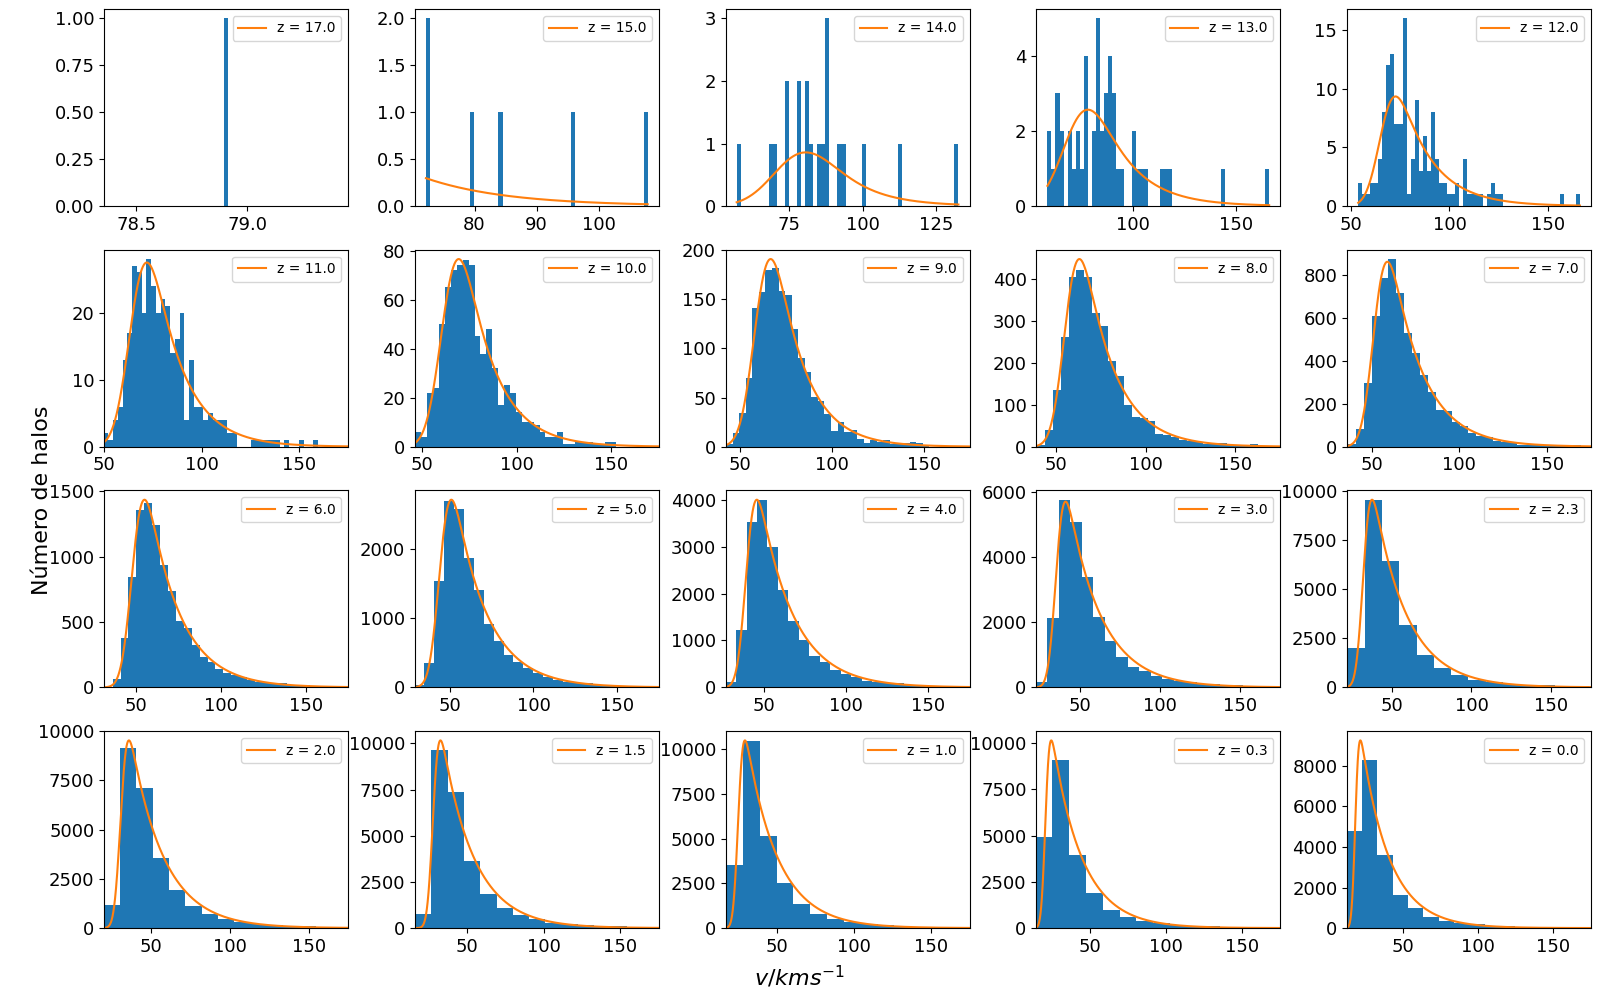
\includegraphics[width = 0.75\linewidth]{RunCanonica/VelDisp_Dist_RunCanonicaSep.png}
    \caption[Dispersión de velocidades]{\footnotesize Se muestra la dispersión de velocidades conforme evoluciona el Universo en una cosmología $\Omega_\lambda = 0.691 $ y $\Omega_0 = 0.309$.Se tienen las distribuciones en los diferentes redshifts empezando en $z=17$ en la parte superior izquierda y terminado en $z=0$ en la parte inferior derecha.}
    \label{fig:Canon-VelDispDistSep}
\end{figure}

\begin{figure}[H]
    \centering
    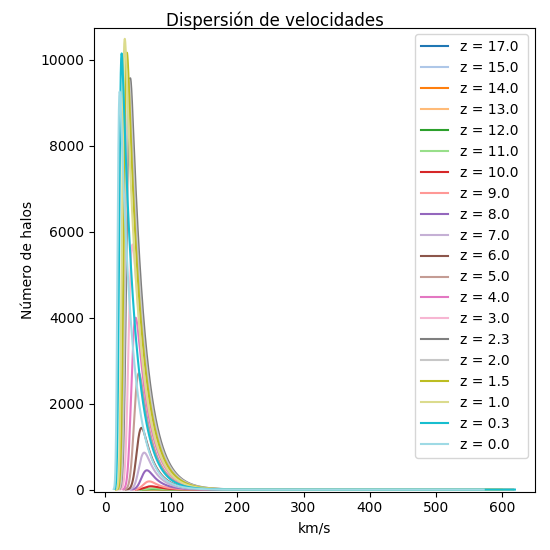
\includegraphics[width = 0.5\linewidth]{RunCanonica/VelDisp_Dist_RunCanonica.png}
    \caption[Distribución de la dispersión de velocidades]{\footnotesize Mostramos la dispersion de velocidades de los halos de materia oscura en un Universo $\Omega_\lambda = 0.691 $, $\Omega_0 = 0.309$.}
    \label{fig:Canon-VelDispDist}
\end{figure}

\begin{figure}[H]
    \centering
    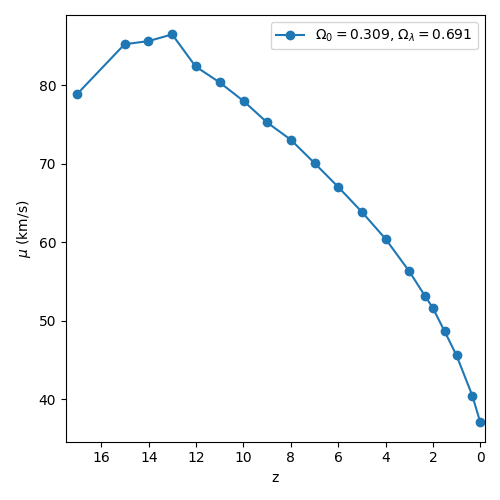
\includegraphics[width = 0.4\linewidth]{RunCanonica/VelDisp_Mean_RunCanonica.png}
    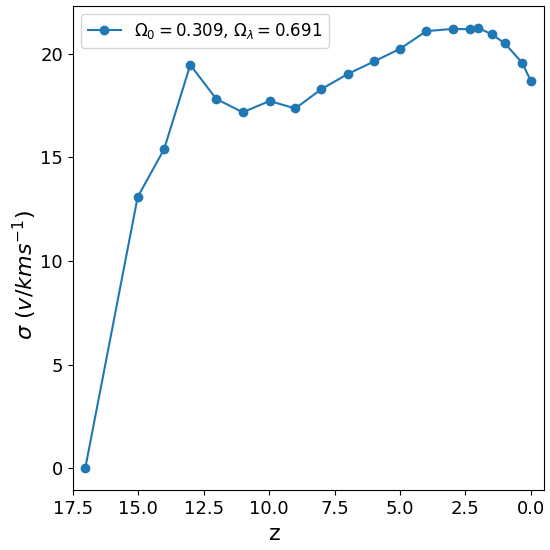
\includegraphics[width = 0.4\linewidth]{RunCanonica/VelDisp_Std_RunCanonica.png}
    \caption[Media y desviación estándar de la dispersión de velocidades]{\footnotesize En la izquierda mostramos la media de la dispersión de velocidades de los halos de materia oscura y en la derecha se muestra su desviación estándar a lo largo de la evolución del Universo.}
    \label{fig:Canon-VelDispStats}
\end{figure}

Finalmente, la figura \ref{fig:CanonRunDensityMap} muestra a lo que conocemos como la \emph{Cosmic Web} vista desde un plano. Se ve el mapa de densidad de la simulación del Universo en diferentes redshifts. En los redshift altos (viendo mas al pasado) se observan nubes difusas donde no hay una estructura, mientras que los redshift bajos (mas al presente) se observan estructuras mejor definidos y con el tiempo vemos que hay un aumento en la cantidad de estructura que se observa.

\begin{figure}[H]
    \centering

    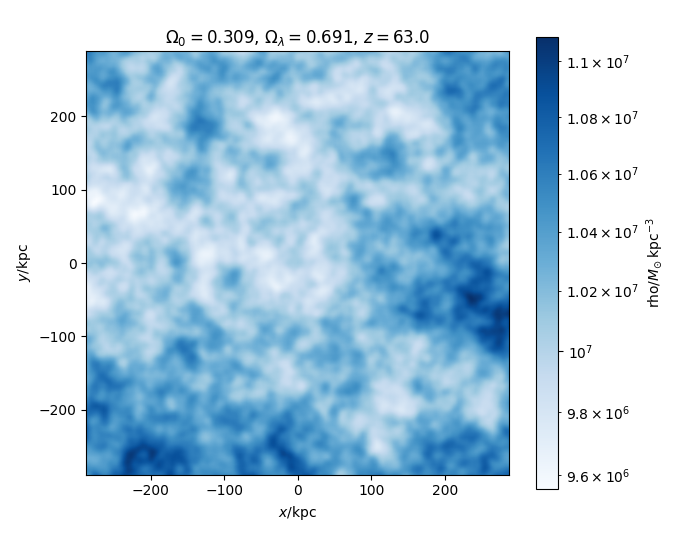
\includegraphics[width = 0.33\linewidth]{RunCanonica/RunCanonZ63Rho.png}   %snap 000 z=63
    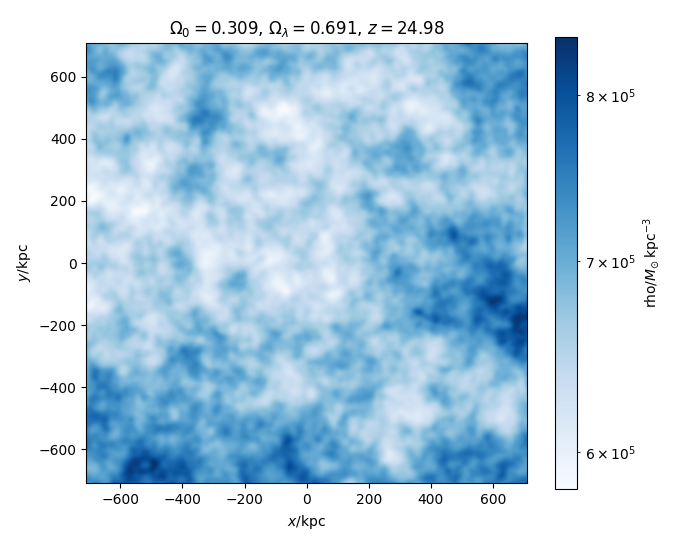
\includegraphics[width = 0.33\linewidth]{RunCanonica/RunCanonZ25Rho.png}   %snap 005 z=25
    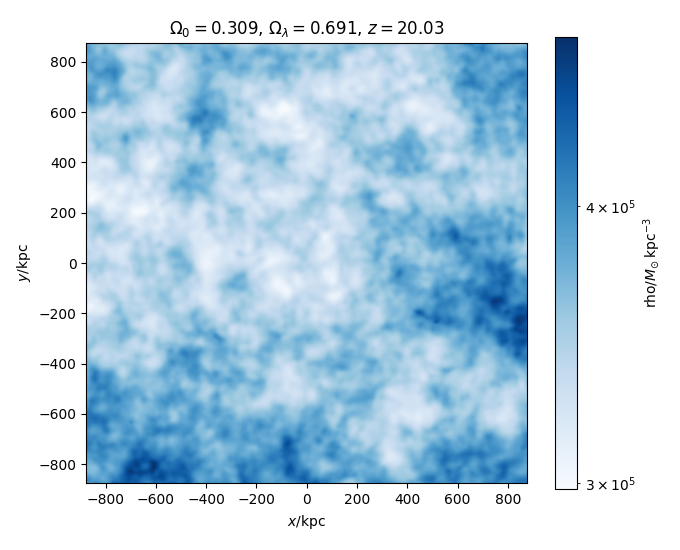
\includegraphics[width = 0.32\linewidth]{RunCanonica/RunCanonZ20Rho.png}   %snap 010 z=20
    \\
    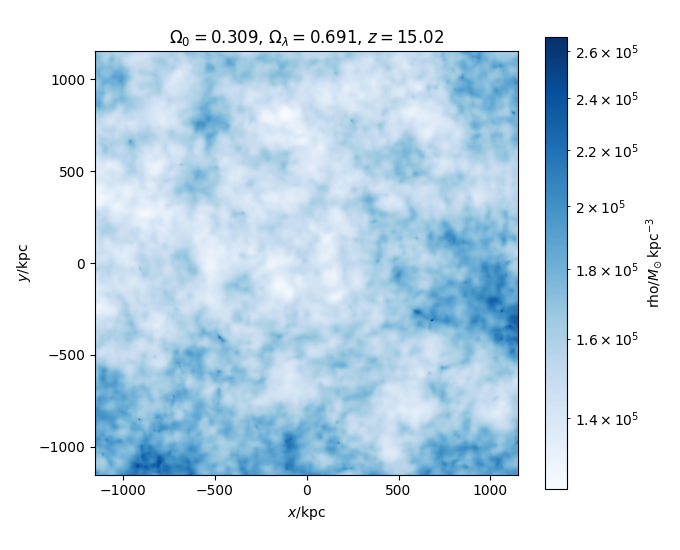
\includegraphics[width = 0.33\linewidth]{RunCanonica/RunCanonZ15Rho.png}   %snap 015 z=15
    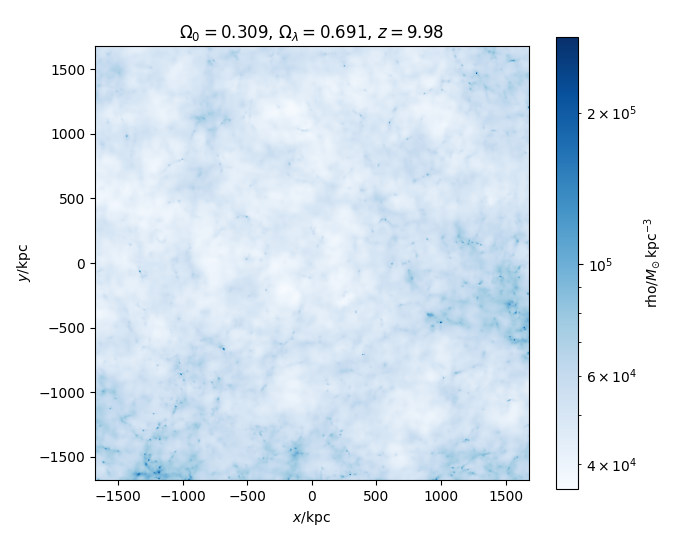
\includegraphics[width = 0.33\linewidth]{RunCanonica/RunCanonZ10Rho.png}   %snap 020 z=10
    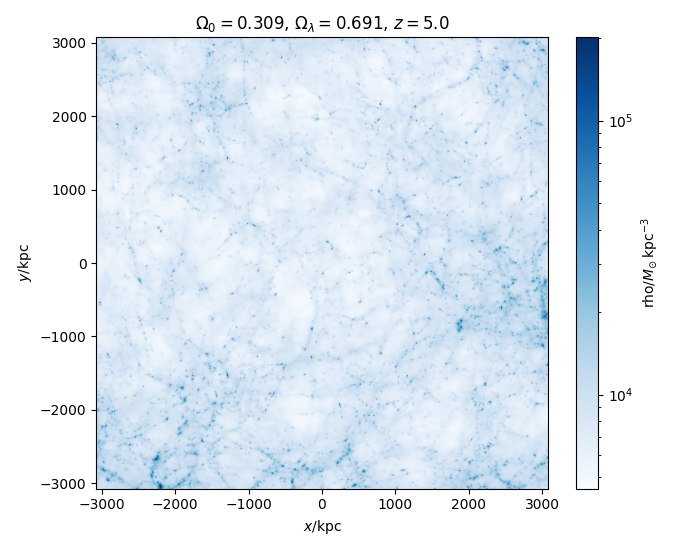
\includegraphics[width = 0.32\linewidth]{RunCanonica/RunCanonZ5Rho.png}    %snap 025 z=5
    \\
    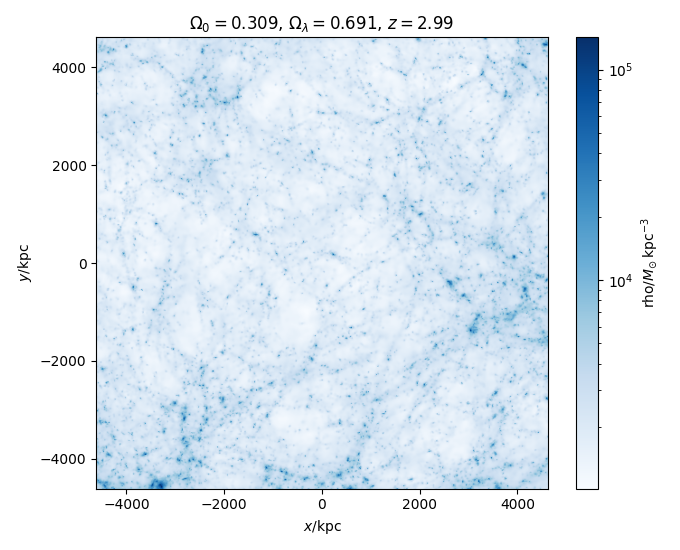
\includegraphics[width = 0.33\linewidth]{RunCanonica/RunCanonZ3Rho.png}    %snap 027 z=3
    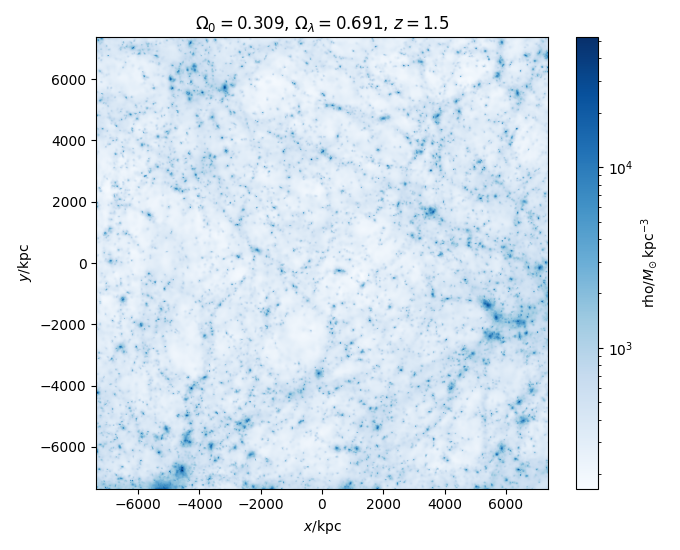
\includegraphics[width = 0.33\linewidth]{RunCanonica/RunCanonZ1_5Rho.png}  %snap 030 z=1.5
    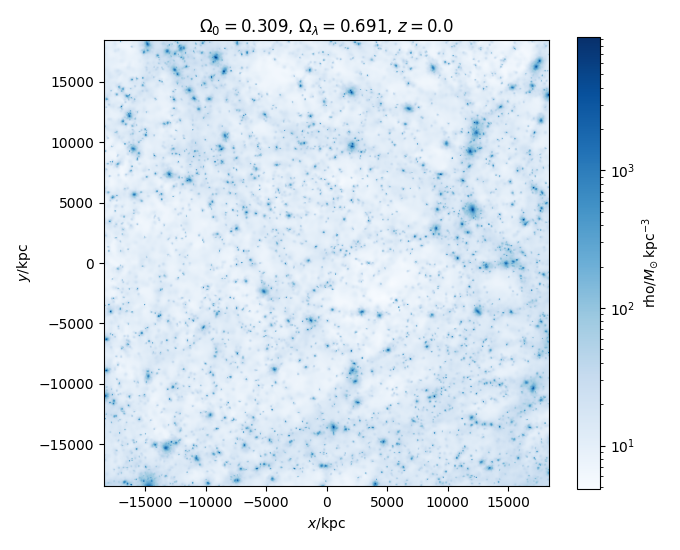
\includegraphics[width = 0.32\linewidth]{RunCanonica/RunCanonZ0Rho.png}    %snap 033 z=0
    \caption[Mapa de densidad de un Universo en en diferentes redshift]{ \footnotesize Mapa de densidad de la simulación en diferentes redshifts de una cosmología $\Omega_\lambda = 0.691 $, $\Omega_0 = 0.309$. }
    \label{fig:CanonRunDensityMap}
\end{figure}

%====================================================================================================================
%=====================================  RUN INVERTIDA  ==============================================================
%====================================================================================================================
\subsection{Universo con cosmología  \texorpdfstring{$\Omega_\lambda = 0.309$, $\Omega_0 = 0.691$ }{Omega lambda = 0.309, Omega 0 = 0.691} }
Hemos estudiado un Universo con las densidades mas aceptadas, pero como cambia si las densidades cambian, para este caso que sucede si invertimos las densidades pero dejamos el Universo plano. Primeramente podemos apreciar en la figura \ref{fig:Invertida-TotalHalos} que los halos se empiezan a formar en redshift $z=14$ pero tiene un comportamiento similar a la cosmología anterior, teniendo el pico en la cantidad de halos alrededor del redshift $z=2$. 

\begin{figure}[H]
    \centering
    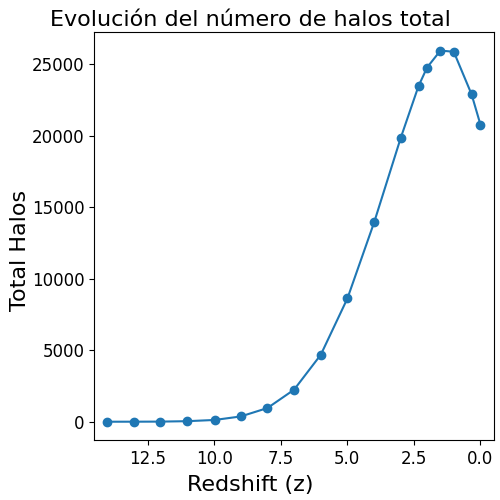
\includegraphics[scale = 0.5]{RunInvertida/TotalHalos_RunInvertida.png}
    \caption[Evolución del número de halos en un Universo $\Omega_\lambda = 0.309 $, $\Omega_0 = 0.691$]{\footnotesize Se muestra el numero de halos y como cambia la cantidad conforme evoluciona el Universo en una cosmología $\Omega_\lambda = 0.309 $ y $\Omega_0 = 0.691$.}    
    \label{fig:Invertida-TotalHalos}
\end{figure}

La distribución de masa de los halos se ve en la figura \ref{fig:Invertida-MassDist} a largo de la evolución. Podemos ver poca estructura con masas mayores a $10^{12}M_\odot$ y mayor parte de la masa entre $10^{10.3}$ y $10^{11}M_\odot$. Ademas en  \ref{fig:Invertida-MassStats} vemos que la media muestra un incremento en la masa de los halos, el que va de $10^{10.8} M\odot$ en $z=13$ hasta $10^{11.1}M_\odot$ en $z=0$. Esto es un incremento de aproximadamente un orden de magnitud. Mientras la desviación tiene un incremento aproximado de $10^{0.1}M_\odot$ en $z=13$ a $10^{0.5}M_\odot$ en $z=0$. 

\begin{figure}[H]
    \centering
    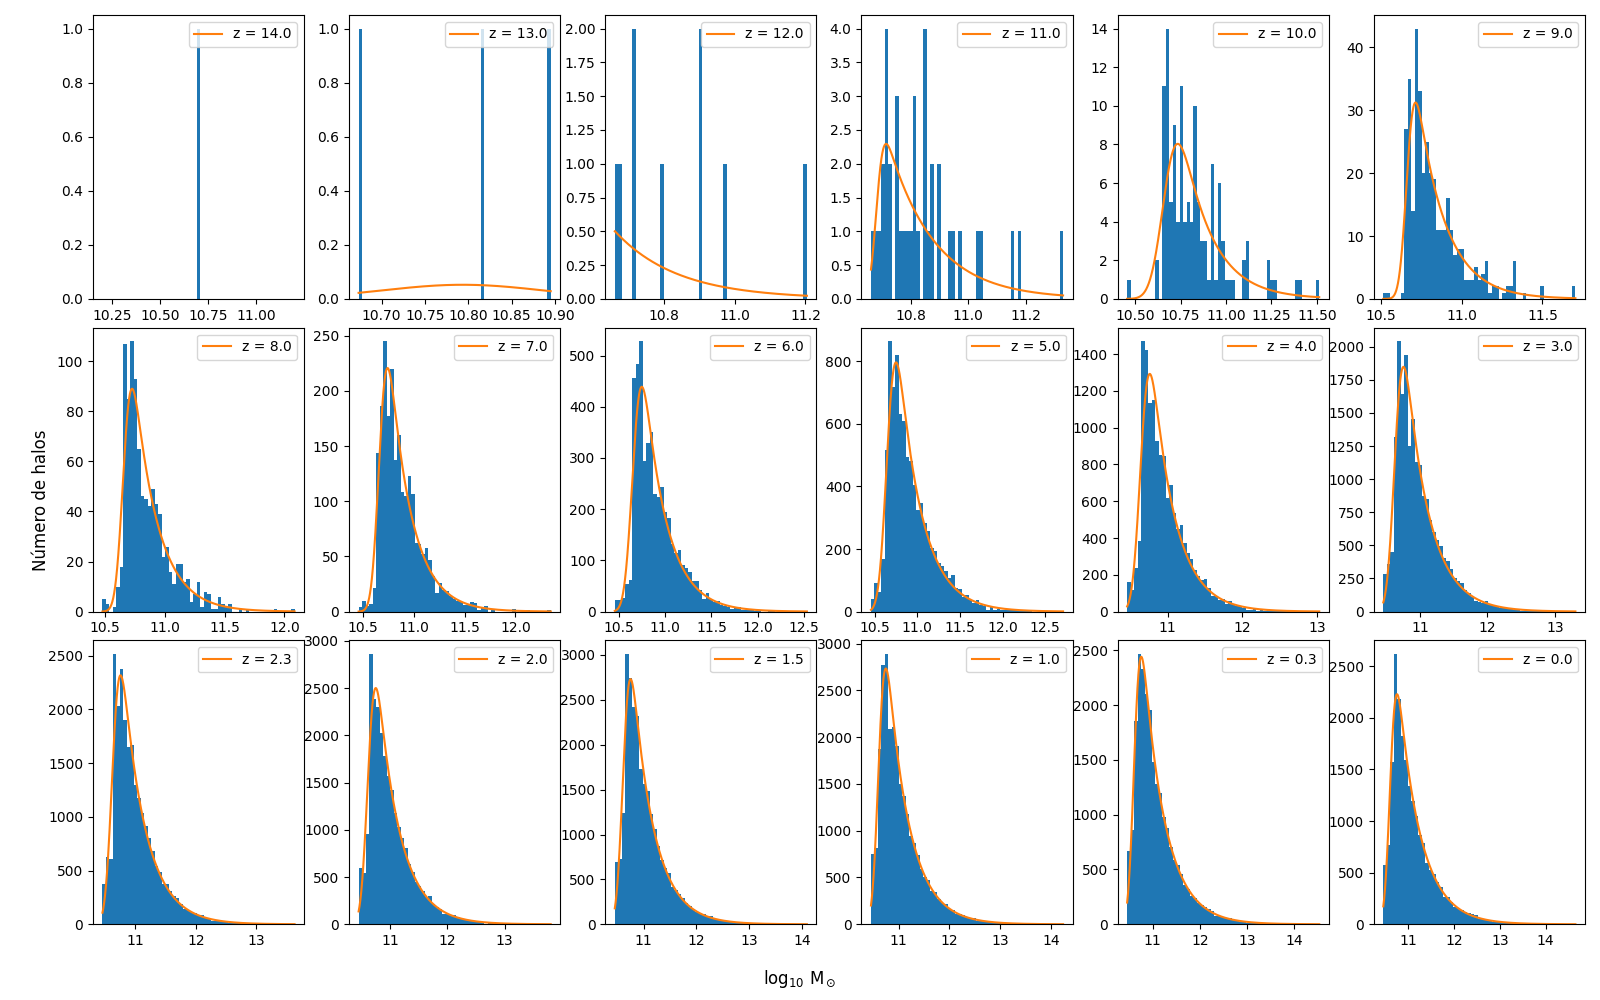
\includegraphics[width = 0.8\linewidth]{RunInvertida/Mass_Dist_RunInvertidaSep.png}
    \caption[Distribución de masa]{\footnotesize Se muestra la distribución de la masa conforme evoluciona el Universo en una cosmología $\Omega_\lambda = 0.309 $ y $\Omega_0 = 0.691$. Se observa como aumentan la cantidad de halos cada vez mas masivos.}
    \label{fig:Invertida-MassDistSep}
\end{figure}

\begin{figure}[H]
    \centering
    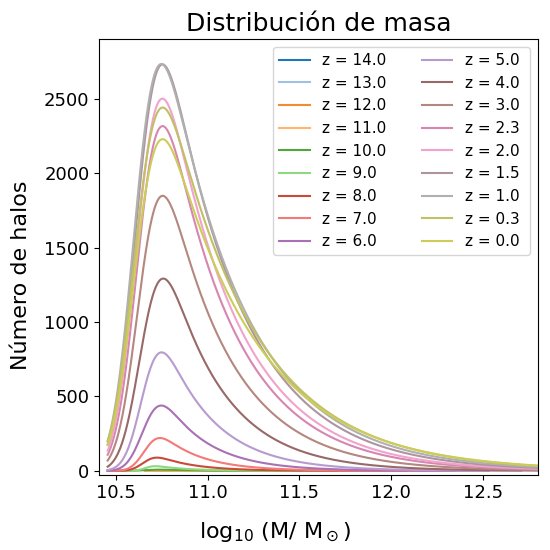
\includegraphics[width = 0.5\linewidth]{RunInvertida/Mass_Dist_RunInvertida.png}
    \caption[Comparación de distribución de masa]{\footnotesize Comparación de las distribuciones de masa durante la evolución del Universo $\Omega_\lambda = 0.309 $, $\Omega_0 = 0.691$. Se observa como crece la cantidad de halos de materia oscura, asi como el tamaño de estos.}
    \label{fig:Invertida-MassDist}
\end{figure}

\begin{figure}[H]
    \centering
    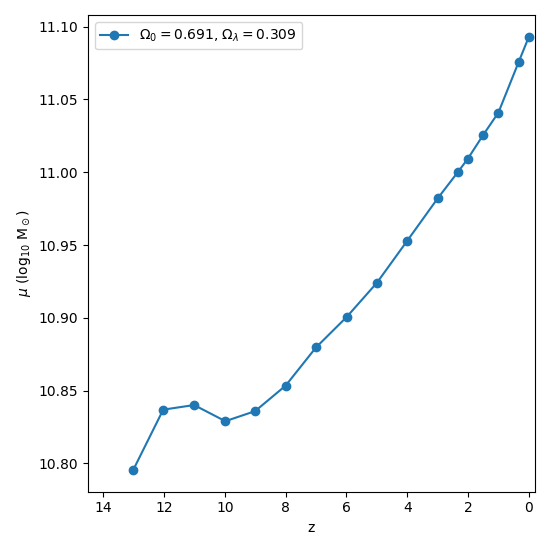
\includegraphics[width = 0.4\linewidth]{RunInvertida/MassMean_RunInvertida.png}
    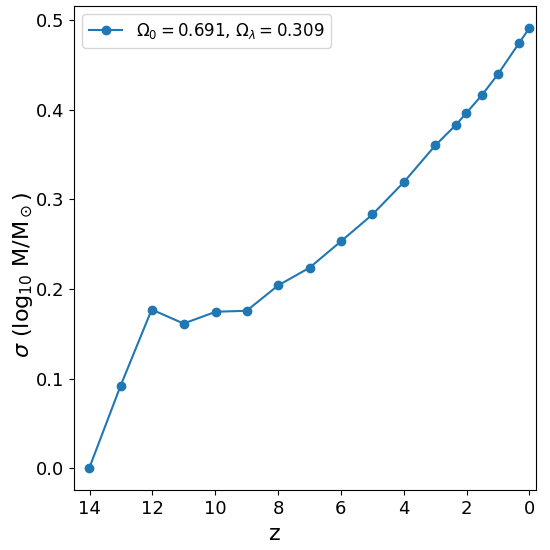
\includegraphics[width = 0.4\linewidth]{RunInvertida/MassStd_RunInvertida.png}
    \caption[Media y desviación estándar de la distribución de masa]{\footnotesize En la izquierda se muestra la masa media de los halos de materia oscura y se observa como cambia durante la evolución del Universo. En la derecha se muestra la desviación estándar de la masa, la cual nos muestra la variedad que hay de los halos de materia oscura.}
    \label{fig:Invertida-MassStats}
\end{figure}

Ahora hablemos del tamaño de estas estructuras, empezando con el radio que contiene la mitad de la masa. En la figura \ref{fig:Invertida-HalfMassRadDistSep} y \ref{fig:Invertida-HalfMassRadDist} vemos que tenemos halos que tienen radios desde $10^{0.35}$ kpc hasta $10^{2.5}$ kpc a lo largo de la evolución de los halos. Vemos en la figura \ref{fig:Invertida-HalfMassRadStats} que el radio crece con el tiempo teniendo un crecimiento desde $10^{0.53}$kpc en las primeras estructuras hasta $10^{1.5}$kpc en el presente. También vemos que las primeras estructuras tienen desviaciones de entre $10^{0.08}$ y $10^{0.15}$kpc mientras que las mas recientes estaban entre $10^{0.15}$ y $10^{0.19}$ kpc.

\begin{figure}[H]
    \centering
    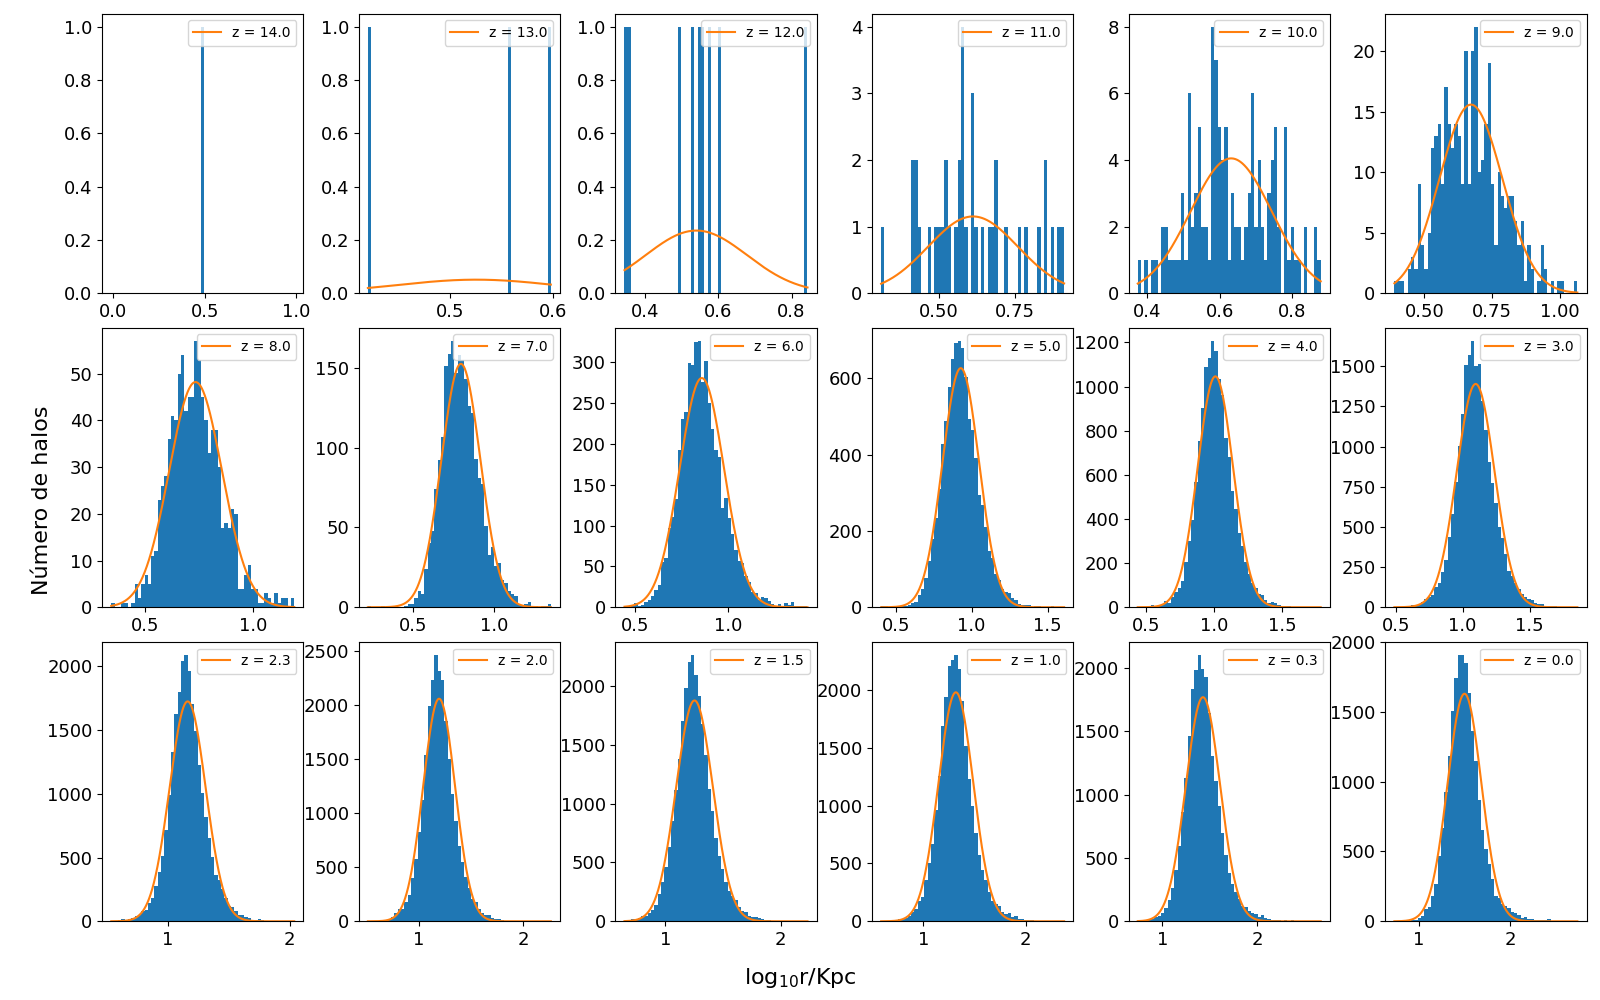
\includegraphics[width = 0.75\linewidth]{RunInvertida/HalfMassRad_Dist_RunInvertidaSep.png}
    \caption[Radio que contiene la mitad de la masa]{\footnotesize Se muestra el radio que contiene la mitad de la masa conforme evoluciona el Universo en una cosmología $\Omega_\lambda = 0.309 $ y $\Omega_0 = 0.691$.}
    \label{fig:Invertida-HalfMassRadDistSep}
\end{figure}

\begin{figure}[H]
    \centering
    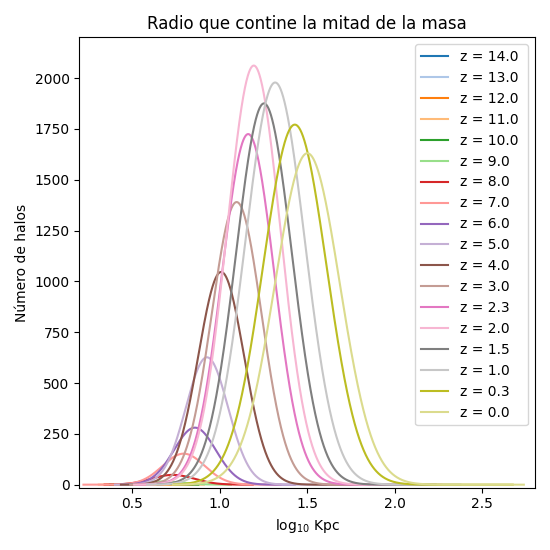
\includegraphics[width = 0.5\linewidth]{RunInvertida/HalfMassRad_Dist_RunInvertida.png}
    \caption[Distribución del Radio que contiene la mitad de la masa]{\footnotesize Comparación de las distribuciones del radio que contiene la mitad de la masa de los halos de materia oscura de un Universo $\Omega_\lambda = 0.309 $, $\Omega_0 = 0.691$.}
    \label{fig:Invertida-HalfMassRadDist}
\end{figure}

\begin{figure}[H]
    \centering
    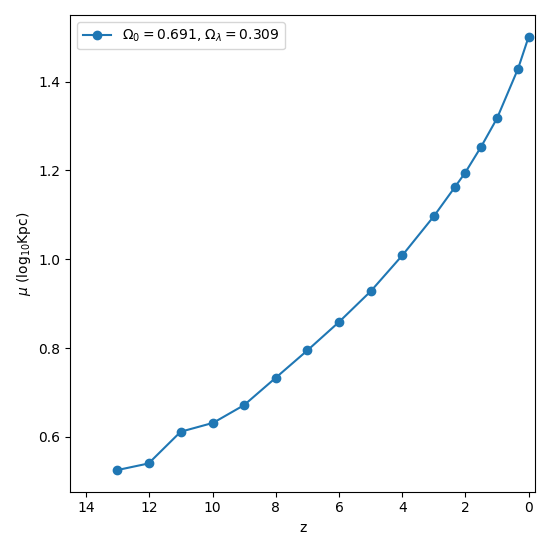
\includegraphics[width = 0.4\linewidth]{RunInvertida/HalfMassRad_Mean_RunInvertida.png}
    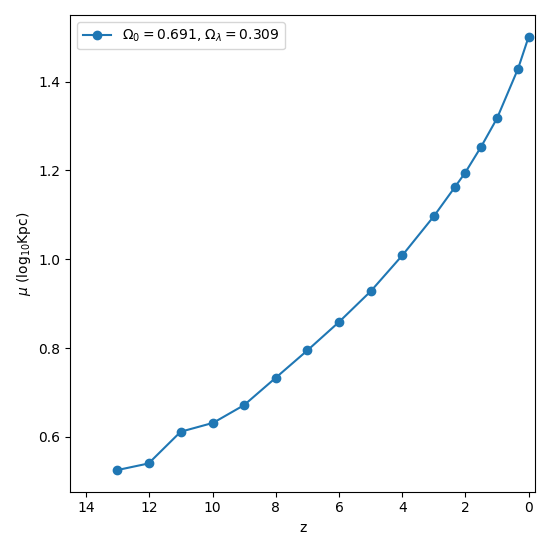
\includegraphics[width = 0.4\linewidth]{RunInvertida/HalfMassRad_Std_RunInvertida.png}
    \caption[Media y desviación estándar del radio de la mitad de la masa]{\footnotesize En la izquierda mostramos la media del radio que contiene la mitad de la masa de los halos de materia oscura y en la derecha se muestra su desviación estándar a lo largo de la evolución del Universo.}
    \label{fig:Invertida-HalfMassRadStats}
\end{figure}

Ahora veamos el comportamiento del radio asociado con la velocidades circular. En las figuras \ref{fig:Invertida-VMaxRadDistSep} y \ref{fig:Invertida-VMaxRadDist} observamos que a lo largo de la evolución de las estructuras tenemos halos con radios que van desde los $2$kpc hasta los $600$kpc. Vemos que la gran mayoría de los halos son halos con tamaños menores a $100$kpc mas al presente y menores a $10$kpc en los redshifts mas altos. En la figura \ref{fig:Invertida-VMaxRadStats} vemos que la media va desde los $4.28$kpc con una desviación de $0.02$kpc en $z=13$ hasta $30.5$kpc con una desviación de $18.7$kpc en $z=0$.

\begin{figure}[H]
    \centering
    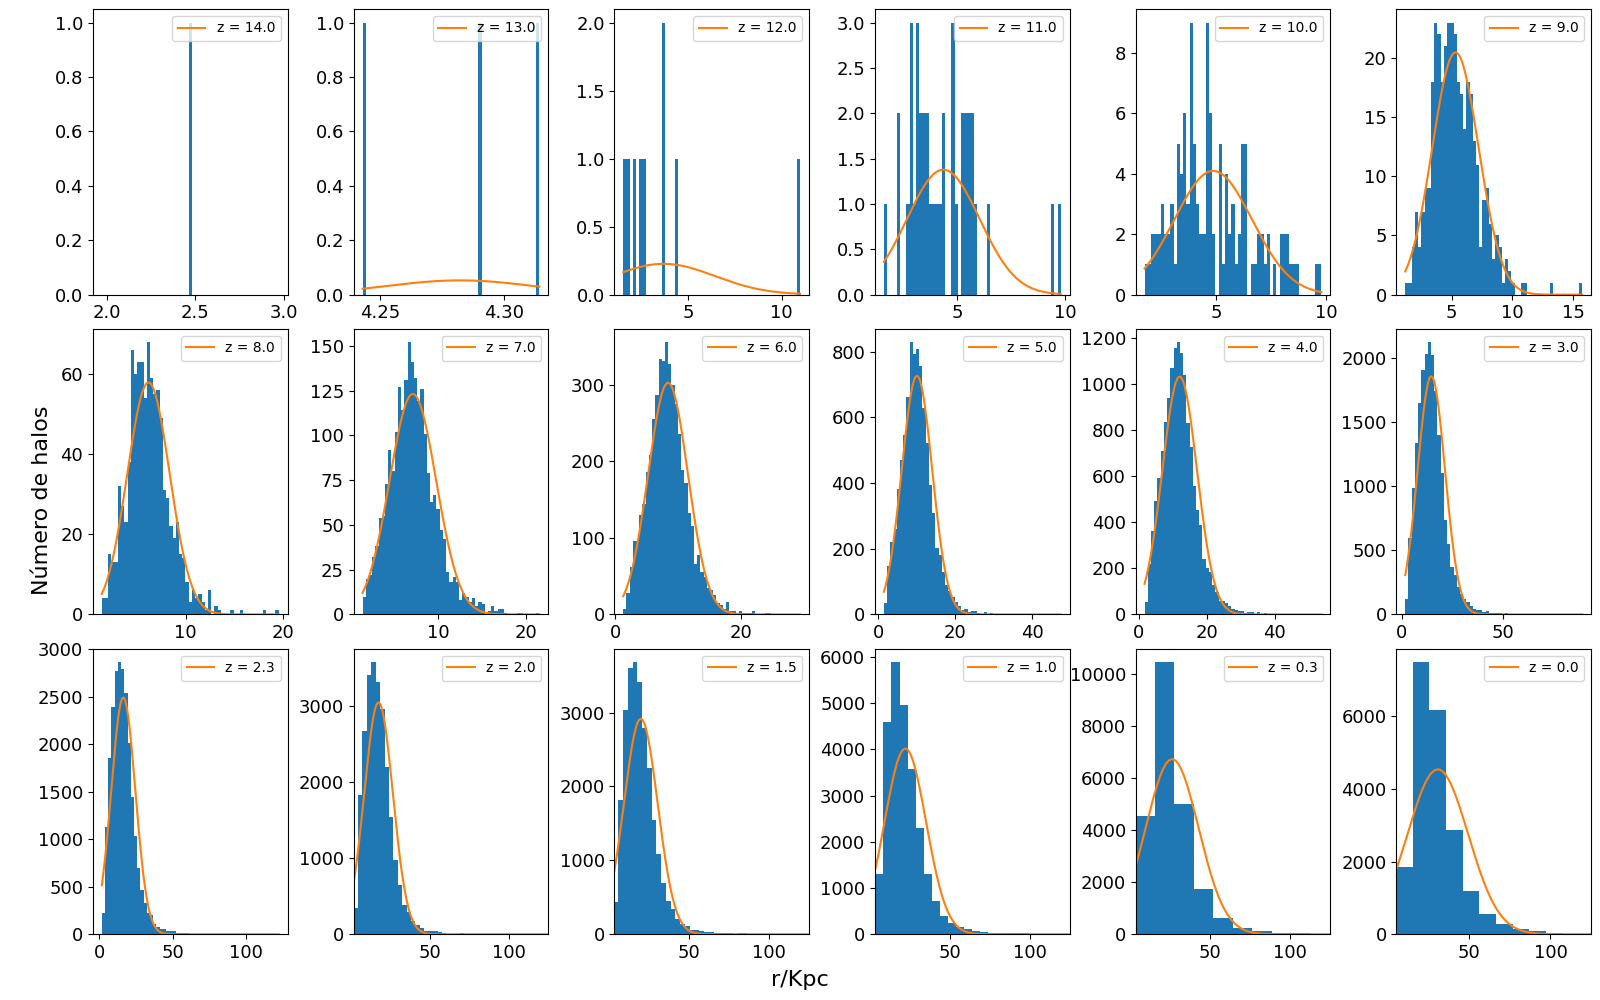
\includegraphics[width = 0.75\linewidth]{RunInvertida/VMaxRad_Dist_RunInvertidaSep.png}
    \caption[Radio donde se alcanza la velocidad máxima radial]{\footnotesize Se muestra el radio donde se alcanza la velocidad máxima radial conforme evoluciona el Universo en una cosmología $\Omega_\lambda = 0.309 $ y $\Omega_0 = 0.691$. Se observa como aumentan la cantidad de halos cada vez mas masivos.}
    \label{fig:Invertida-VMaxRadDistSep}
\end{figure}

\begin{figure}[H]
    \centering
    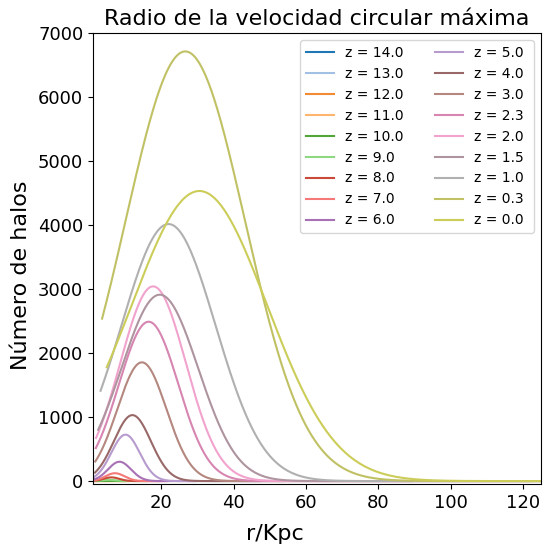
\includegraphics[width = 0.5\linewidth]{RunInvertida/VMaxRad_Dist_RunInvertida.png}
    \caption[Distribución del radio donde se alcanza la velocidad máxima radial]{\footnotesize Comparación de las distribuciones del radio donde se alcanza la velocidad máxima radial de los halos de materia oscura de un Universo $\Omega_\lambda = 0.309 $, $\Omega_0 = 0.691$.}
    \label{fig:Invertida-VMaxRadDist}
\end{figure}

\begin{figure}[H]
    \centering
    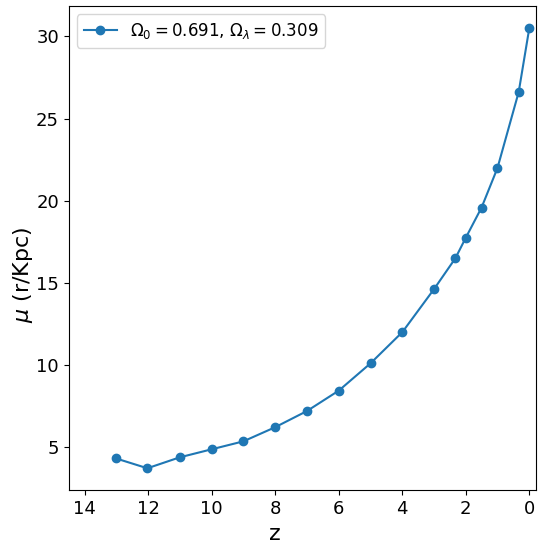
\includegraphics[width = 0.4\linewidth]{RunInvertida/VMaxRad_Mean_RunInvertida.png}
    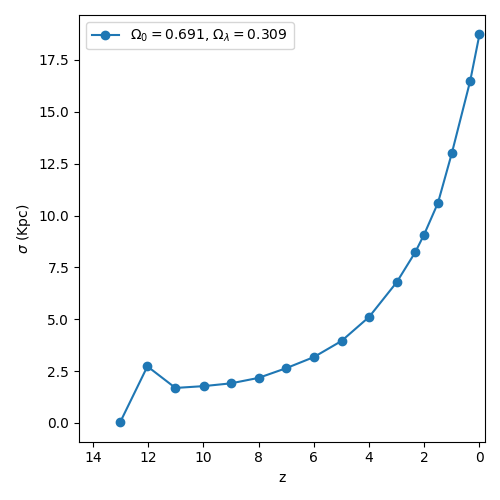
\includegraphics[width = 0.4\linewidth]{RunInvertida/VMaxRad_Std_RunInvertida.png}
    \caption[Media y desviación estándar del Radio donde se alcanza la velocidad máxima radial]{\footnotesize En la izquierda mostramos la media del radio donde se alcanza la velocidad máxima radial de los halos de materia oscura y en la derecha se muestra su desviación estándar a lo largo de la evolución del Universo.}
    \label{fig:Invertida-VMaxRadStats}
\end{figure}

Seguimos con la velocidad circular máxima que se alcanza en estos radios. Podemos apreciar que las velocidades circulares van de los rangos de los $20$km/s hasta los $1400$km/s donde vemos la gran mayoría de los halos en los rangos de $100$km/s y $200$km/s, como se muestra en las figuras \ref{fig:Invertida-VelMaxDistSep} y \ref{fig:Invertida-VelMaxDist}. Lo que podemos ver en la figura \ref{fig:Invertida-VelMaxStats} es que la velocidad  media disminuye rápidamente desde $207.01$km/s con una desviación de $13.71$km/s en $z=13$ hasta que alcanza $106.06$km/s con una desviación de $47.34$km/s en $z=0$. 

\begin{figure}[H]
    \centering
    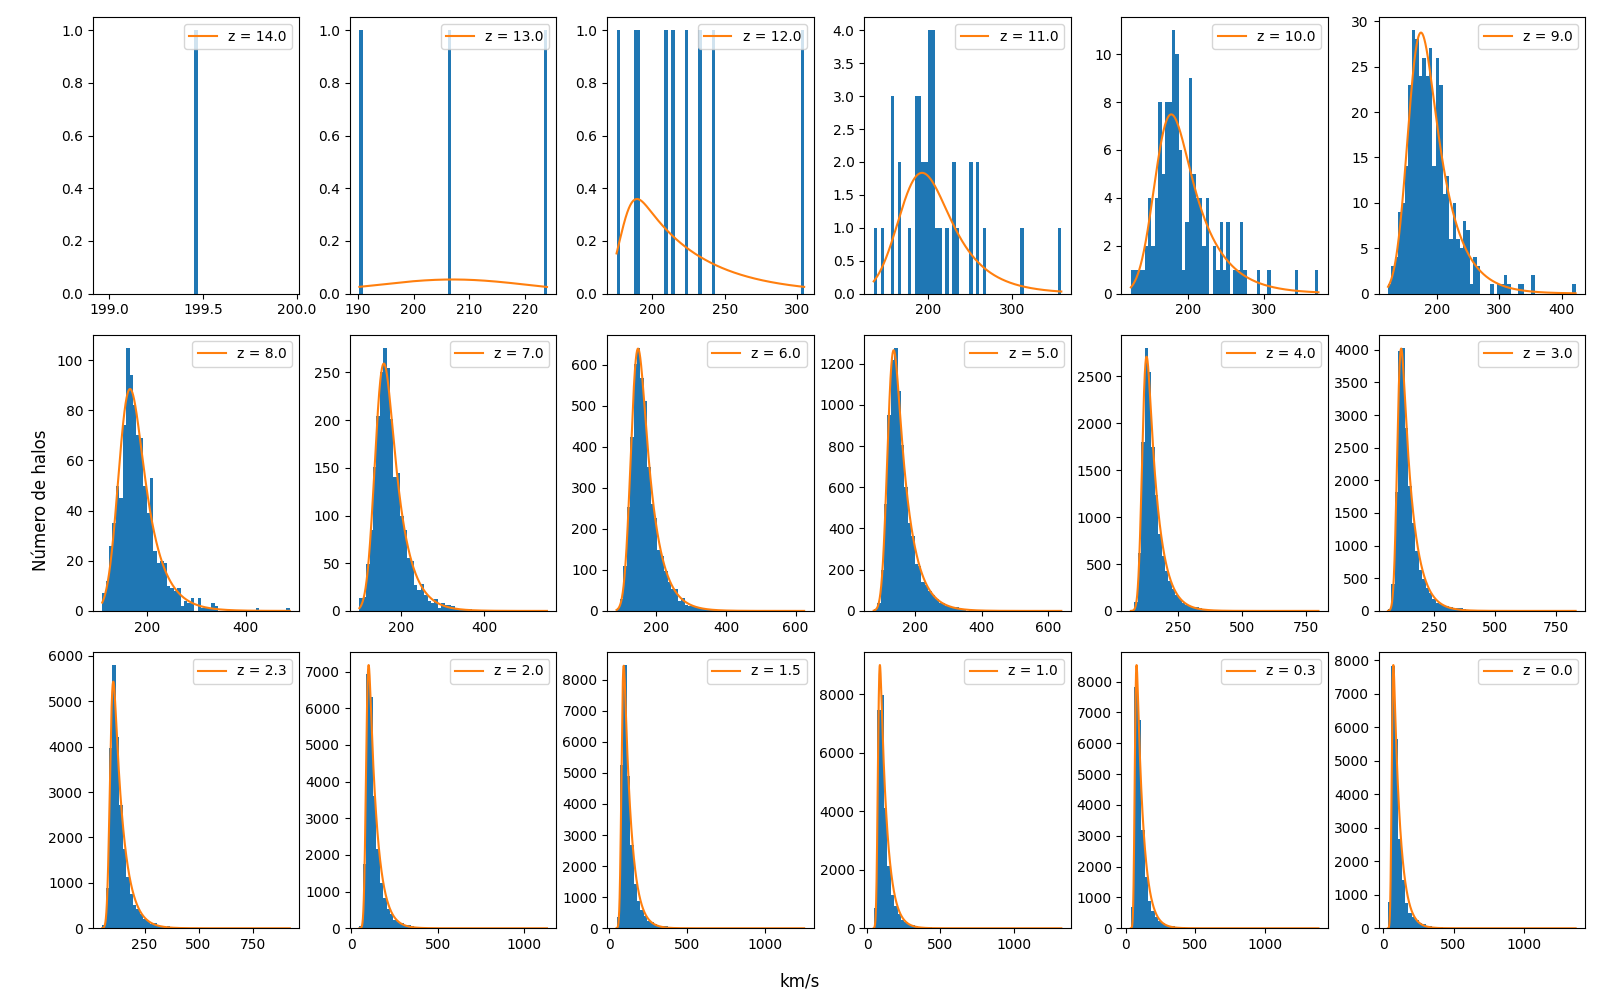
\includegraphics[width = 0.75\linewidth]{RunInvertida/VelMax_Dist_RunInvertidaSep.png}
    \caption[Velocidad circular máxima]{\footnotesize Se muestra la velocidad circular máxima conforme evoluciona el Universo en una cosmología $\Omega_\lambda = 0.309 $ y $\Omega_0 = 0.691$.}
    \label{fig:Invertida-VelMaxDistSep}
\end{figure}

\begin{figure}[H]
    \centering
    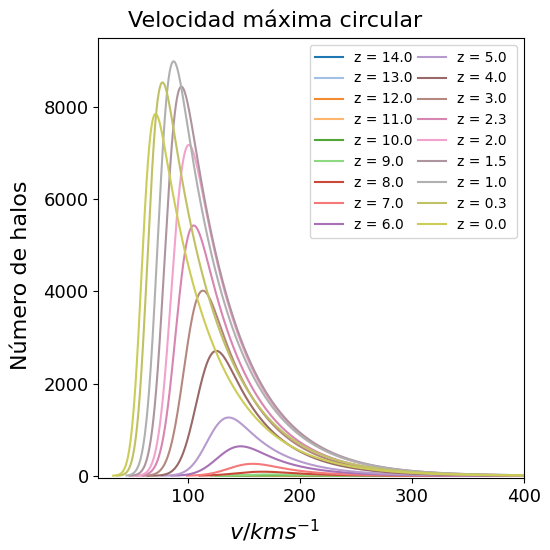
\includegraphics[width = 0.5\linewidth]{RunInvertida/VelMax_Dist_RunInvertida.png}
    \caption[Distribución de la velocidad circular máxima]{\footnotesize Comparación de las distribuciones de la velocidad circular máxima de los halos de materia oscura de un Universo $\Omega_\lambda = 0.309 $, $\Omega_0 = 0.691$.}
    \label{fig:Invertida-VelMaxDist}
\end{figure}

\begin{figure}[H]
    \centering
    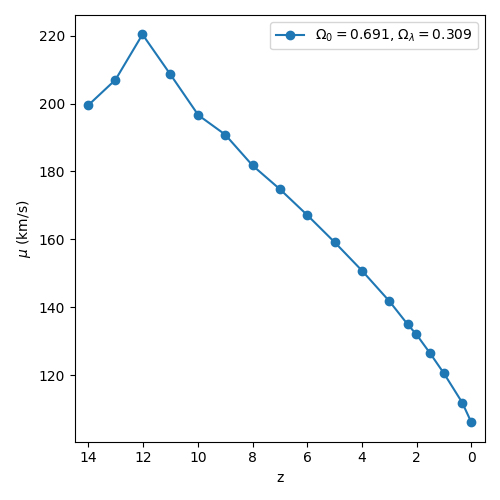
\includegraphics[width = 0.4\linewidth]{RunInvertida/VelMax_Mean_RunInvertida.png}
    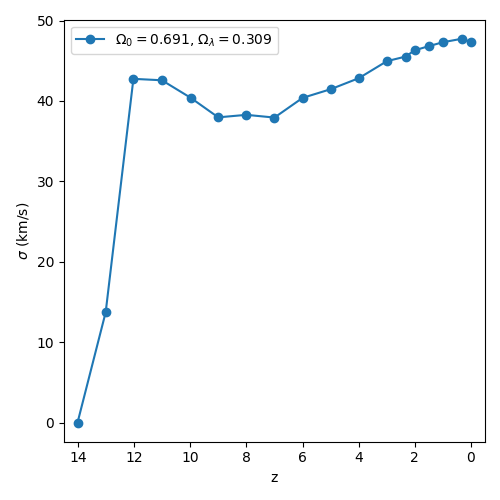
\includegraphics[width = 0.4\linewidth]{RunInvertida/VelMax_Std_RunInvertida.png}
    \caption[Media y desviación estándar de la velocidad circular máxima]{\footnotesize En la izquierda mostramos la media de la velocidad circular máxima de los halos de materia oscura y en la derecha se muestra su desviación estándar a lo largo de la evolución del Universo.}
    \label{fig:Invertida-VelMaxStats}
\end{figure}


La dispersión de velocidades de estos halos esta en los rangos de $17$km/s a los $857$km/s a lo largo de la evolución de los halos. Vemos en las figuras \ref{fig:Invertida-VelDispDistSep} y \ref{fig:Invertida-VelDispDist} que en los $z$ altos vemos que que la mayor parte de los halos se encuentran en el rango de los $100$km/s a los $150$km/s con picos en los $200$km/s y $400$km/s, mientras que en los $z$ bajos vemos los rango que van de $50$km/s y $150$km/s con los picos entre los $400$km/s y $857$km/s. En la figura \ref{fig:Invertida-VelDispStats} observamos que la dispersión de velocidades media disminuye desde los $114.45$km/s con una desviación de $7.96$km/s en $z=14$ a $54.03$km/s con una desviación de $26.70$km/s en $z=0$.


\begin{figure}[H]
    \centering
    \includegraphics[width = 0.75\linewidth]{RunInvertida/VelDisp_Dist_RunInvertidaSep.png}
    \caption[Dispersión de velocidades]{\footnotesize Se muestra la dispersión de velocidades conforme evoluciona el Universo en una cosmología $\Omega_\lambda = 0.309 $ y $\Omega_0 = 0.691$.}
    \label{fig:Invertida-VelDispDistSep}
\end{figure}

\begin{figure}[H]
    \centering
    \includegraphics[width = 0.5\linewidth]{RunInvertida/VelDisp_Dist_RunInvertida.png}
    \caption[Distribución de la dispersión de velocidades]{\footnotesize Comparación de las distribuciones de la dispersión de velocidades de los halos de materia oscura de un Universo $\Omega_\lambda = 0.309 $, $\Omega_0 = 0.691$.}
    \label{fig:Invertida-VelDispDist}
\end{figure}

\begin{figure}[H]
    \centering
    \includegraphics[width = 0.4\linewidth]{RunInvertida/VelDisp_Mean_RunInvertida.png}
    \includegraphics[width = 0.4\linewidth]{RunInvertida/VelDisp_Std_RunInvertida.png}
    \caption[Media y desviación estándar de la dispersión de velocidades]{\footnotesize En la izquierda mostramos la media de la dispersión de velocidades de los halos de materia oscura y en la derecha se muestra su desviación estándar a lo largo de la evolución del Universo.}
    \label{fig:Invertida-VelDispStats}
\end{figure}

La figura \ref{fig:Invertida-DensityMap} muestra la el mapa de densidad de un Universo $\Omega_\lambda = 0.309 $ $\Omega_0 = 0.691$, donde podemos ver la estructura que describimos  en los diferentes puntos de su evolución vista desde un plano .
\begin{figure}[H]
    \centering

    \includegraphics[width = 0.33\linewidth]{RunInvertida/RunInvertidaZ63.png}   %snap 000 z=63
    \includegraphics[width = 0.33\linewidth]{RunInvertida/RunInvertidaZ25.png}   %snap 005 z=25
    \includegraphics[width = 0.32\linewidth]{RunInvertida/RunInvertidaZ20.png}   %snap 010 z=20
    \\
    \includegraphics[width = 0.33\linewidth]{RunInvertida/RunInvertidaZ15.png}   %snap 015 z=15
    \includegraphics[width = 0.33\linewidth]{RunInvertida/RunInvertidaZ10.png}   %snap 020 z=10
    \includegraphics[width = 0.32\linewidth]{RunInvertida/RunInvertidaZ5.png}    %snap 025 z=5
    \\
    \includegraphics[width = 0.33\linewidth]{RunInvertida/RunInvertidaZ3.png}    %snap 027 z=3
    \includegraphics[width = 0.33\linewidth]{RunInvertida/RunInvertidaZ1_5.png}  %snap 030 z=1.5
    \includegraphics[width = 0.32\linewidth]{RunInvertida/RunInvertidaZ0.png}    %snap 033 z=0
    \caption[Mapa de densidad en en diferentes redshift]{ \footnotesize Mapa de densidad de la simulación en diferentes redshifts de una cosmología $\Omega_\lambda = 0.309 $, $\Omega_0 = 0.691$. }
    \label{fig:Invertida-DensityMap}
\end{figure}

%====================================================================================================================
%=====================================  RUN HALF COSMO  =============================================================
%====================================================================================================================
\subsection{Universo con cosmología \texorpdfstring{$\Omega_\lambda = 0.5$, $\Omega_0 = 0.5$ }{Omega lambda = 0.5, Omega 0 = 0.5} }

Hemos visto que como se comporta un Universo con las densidades mas aceptadas y cuando estas se invierten. Ahora veamos un Universo con las densidades iguales ($\Omega_\lambda = 0.5$, $\Omega_0 = 0.5$). Comencemos viendo como se afecta la cantidad de halos. La figura \ref{fig:HalfCosmo-TotalHalos} muestra que los primeros halos aparecen en $z=15$, además muestra que el máximo de halos en las simulaciones que se alcanza fue de $26242$ halos en $z=1.5$. Observamos un comportamiento similar a las cosmologías anteriores donde vemos un crecimiento rápido hasta que alcanza un máximo y después empieza a disminuir.

\begin{figure}[H]
    \centering
    \includegraphics[scale = 0.5]{RunHalfCosmo/TotalHalos_RunHalfCosmo.png}
    \caption[Evolución del número de halos en un Universo $\Omega_\lambda = 0.5 $, $\Omega_0 = 0.5$]{\footnotesize Se muestra el numero de halos y como cambia la cantidad conforme evoluciona el Universo en una cosmología $\Omega_\lambda = 0.5 $ y $\Omega_0 = 0.5$.}    
    \label{fig:HalfCosmo-TotalHalos}
\end{figure}

La distribución de la masa para esta cosmología se observa en las figuras \ref{fig:HalfCosmo-MassDistSep} y \ref{fig:HalfCosmo-MassDist}. Los rangos de la masa se encuentran entre las $10^{10.3}M_\odot$ a $10^{14.5}M_\odot$ a lo largo de de la evolución del sistema. Las primeras estructuras, las que tienen $z$ altos, tenían masas menores a las $10^{12}M_\odot$ y las estructuras en $z$ pequeños la mayor parte de los halos tenían masas entre $10^{10.5}M_\odot$ y $10^{11.5}M_\odot$. Mientras, la figura \ref{fig:HalfCosmo-MassStats} nos muestra el comportamiento medio durante la evolución. Observamos que la masa media incrementa desde $10^{10.65}M_\odot$ con una desviación de $10^{0.1}M_\odot$ en $z=14$ hasta $10^{10.95}M_\odot$ con una desviación de $10^{0.5}M_\odot$ en $z=0$.

\begin{figure}[H]
    \centering
    \includegraphics[width = 0.8\linewidth]{RunHalfCosmo/Mass_Dist_RunHalfCosmoSep.png}
    \caption[Distribución de masa]{\footnotesize Se muestra la distribución de la masa conforme evoluciona el Universo en una cosmología $\Omega_\lambda = 0.5$ y $\Omega_0 = 0.5$. Se observa como aumentan la cantidad de halos cada vez mas masivos.}
    \label{fig:HalfCosmo-MassDistSep}
\end{figure}

\begin{figure}[H]
    \centering
    \includegraphics[width = 0.5\linewidth]{RunHalfCosmo/Mass_Dist_RunHalfCosmo.png}
    \caption[Comparación de distribución de masa Universo]{\footnotesize Comparación de las distribuciones de masa durante la evolución del Universo $\Omega_\lambda = 0.5$, $\Omega_0 = 0.5$. Se observa como crece la cantidad de halos de materia oscura, asi como el tamaño de estos.}
    \label{fig:HalfCosmo-MassDist}
\end{figure}

\begin{figure}[H]
    \centering
    \includegraphics[width = 0.4\linewidth]{RunHalfCosmo/MassMean_RunHalfCosmo.png}
    \includegraphics[width = 0.4\linewidth]{RunHalfCosmo/MassStd_RunHalfCosmo.png}
    \caption[Media y desviación estándar de la distribución de masa]{\footnotesize En la izquierda se muestra la masa media de los halos de materia oscura y se observa como cambia durante la evolución del Universo. En la derecha se muestra la desviación estándar de la masa, la cual nos muestra la variedad que hay de los halos de materia oscura.}
    \label{fig:HalfCosmo-MassStats}
\end{figure}

En las figuras \ref{fig:HalfCosmo-HalfMassRadDistSep} y \ref{fig:HalfCosmo-HalfMassRadDist} podemos ver el radio que contiene la mitad de la masa de los halos a lo largo de la evolución del Universo. Vemos que los radios se encuentran entre los $10^{0.27}$kpc y $10^{2.72}$kpc donde los primeros halos tienen radios entre los $10^{0.29}$kpc y los $10^{1.61}$ y las estructuras mas recientes tienen la mayor parte de los halos en el rango de $10^{1}$kpc y los $10^{1.75}$. El radio medio tiene un crecimiento de $10^{0.53}$kpc con una desviación de $10^{0.09}$kpc en $z=14$ hasta un radio de $10^{1.49}$kpc con una desviación de $10^{0.18}$kpc en $z=0$.

\begin{figure}[H]
    \centering
    \includegraphics[width = 0.75\linewidth]{RunHalfCosmo/HalfMassRad_Dist_RunHalfCosmoSep.png}
    \caption[Radio que contiene la mitad de la masa]{\footnotesize Se muestra el radio que contiene la mitad de la masa conforme evoluciona el Universo en una cosmología $\Omega_\lambda = 0.5 $ y $\Omega_0 = 0.5$.}
    \label{fig:HalfCosmo-HalfMassRadDistSep}
\end{figure}

\begin{figure}[H]
    \centering
    \includegraphics[width = 0.5\linewidth]{RunHalfCosmo/HalfMassRad_Dist_RunHalfCosmo.png}
    \caption[Distribución del Radio que contiene la mitad de la masa]{\footnotesize Comparación de las distribuciones del radio que contiene la mitad de la masa de los halos de materia oscura en un Universo $\Omega_\lambda = 0.5 $ y $\Omega_0 = 0.5$.}
    \label{fig:HalfCosmo-HalfMassRadDist}
\end{figure}

\begin{figure}[H]
    \centering
    \includegraphics[width = 0.4\linewidth]{RunHalfCosmo/HalfMassRad_Mean_RunHalfCosmo.png}
    \includegraphics[width = 0.4\linewidth]{RunHalfCosmo/HalfMassRad_Std_RunHalfCosmo.png}
    \caption[Media y desviación estándar del radio de la mitad de la masa]{\footnotesize En la izquierda mostramos la media del radio que contiene la mitad de la masa de los halos de materia oscura y en la derecha se muestra su desviación estándar a lo largo de la evolución del Universo.}
    \label{fig:HalfCosmo-HalfMassRadStats}
\end{figure}

Ahora veamos el comportamiento del radio asociado con la velocidades circular. En las figuras \ref{fig:HalfCosmo-VMaxRadDistSep} y \ref{fig:HalfCosmo-VMaxRadDist} observamos que a lo largo de la evolución de las estructuras, tenemos halos con radios que van desde los $1$kpc hasta los $590$kpc. Vemos que la gran mayoría de los halos son halos con tamaños menores a $20$kpc mas al presente y menores a $10$kpc en los redshifts mas altos. En la figura \ref{fig:HalfCosmo-VMaxRadStats} vemos que la media va desde los $3.39$kpc con una desviación de $1.18$kpc en $z=13$ hasta $29.44$kpc con una desviación de $17.95$kpc en $z=0$.

\begin{figure}[H]
    \centering
    \includegraphics[width = 0.75\linewidth]{RunHalfCosmo/VMaxRad_Dist_RunHalfCosmoSep.png}
    \caption[Radio donde se alcanza la velocidad máxima radial]{\footnotesize Se muestra el radio donde se alcanza la velocidad máxima radial conforme evoluciona el Universo en una cosmología $\Omega_\lambda = 0.5$ y $\Omega_0 = 0.5$. Se observa como aumentan la cantidad de halos cada vez mas masivos.}
    \label{fig:HalfCosmo-VMaxRadDistSep}
\end{figure}

\begin{figure}[H]
    \centering
    \includegraphics[width = 0.5\linewidth]{RunHalfCosmo/VMaxRad_Dist_RunHalfCosmo.png}
    \caption[Distribución del radio donde se alcanza la velocidad máxima radial]{\footnotesize Comparación de las distribuciones del radio donde se alcanza la velocidad máxima radial de los halos de materia oscura en un Universo $\Omega_\lambda = 0.5$, $\Omega_0 = 0.5$.}
    \label{fig:HalfCosmo-VMaxRadDist}
\end{figure}

\begin{figure}[H]
    \centering
    \includegraphics[width = 0.4\linewidth]{RunHalfCosmo/VMaxRad_Mean_RunHalfCosmo.png}
    \includegraphics[width = 0.4\linewidth]{RunHalfCosmo/VMaxRad_Std_RunHalfCosmo.png}
    \caption[Media y desviación estándar del Radio donde se alcanza la velocidad máxima radial]{\footnotesize En la izquierda mostramos la media del radio donde se alcanza la velocidad máxima radial de los halos de materia oscura y en la derecha se muestra su desviación estándar a lo largo de la evolución del Universo.}
    \label{fig:HalfCosmo-VMaxRadStats}
\end{figure}

Seguimos con la velocidad circular máxima que se alcanza en estos radios. Podemos apreciar que las velocidades circulares van de los rangos de los $25$km/s hasta los $1216$km/s donde vemos la gran mayoría de los halos en los rangos de $30$km/s y $175$km/s, como se muestra en las figuras \ref{fig:HalfCosmo-VelMaxDistSep} y \ref{fig:HalfCosmo-VelMaxDist}. Lo que podemos ver en la figura \ref{fig:HalfCosmo-VelMaxStats} es que la velocidad  media disminuye rápidamente desde $177.53$km/s con una desviación de $2.14$km/s en $z=15$ hasta que alcanza $92.14$km/s con una desviación de $41.30$km/s en $z=0$. 

\begin{figure}[H]
    \centering
    \includegraphics[width = 0.75\linewidth]{RunHalfCosmo/VelMax_Dist_RunHalfCosmoSep.png}
    \caption[Velocidad circular máxima]{\footnotesize Se muestra la velocidad circular máxima conforme evoluciona el Universo en una cosmología $\Omega_\lambda = 0.5 $ y $\Omega_0 = 0.5$.}
    \label{fig:HalfCosmo-VelMaxDistSep}
\end{figure}

\begin{figure}[H]
    \centering
    \includegraphics[width = 0.5\linewidth]{RunHalfCosmo/VelMax_Dist_RunHalfCosmo.png}
    \caption[Distribución de la velocidad circular máxima]{\footnotesize Comparación de las distribuciones de la velocidad circular máxima de los halos de materia oscura en un Universo $\Omega_\lambda = 0.5 $, $\Omega_0 = 0.5$.}
    \label{fig:HalfCosmo-VelMaxDist}
\end{figure}

\begin{figure}[H]
    \centering
    \includegraphics[width = 0.4\linewidth]{RunHalfCosmo/VelMax_Mean_RunHalfCosmo.png}
    \includegraphics[width = 0.4\linewidth]{RunHalfCosmo/VelMax_Std_RunHalfCosmo.png}
    \caption[Media y desviación estándar de la velocidad circular máxima]{\footnotesize En la izquierda mostramos la media de la velocidad circular máxima de los halos de materia oscura y en la derecha se muestra su desviación estándar a lo largo de la evolución del Universo.}
    \label{fig:HalfCosmo-VelMaxStats}
\end{figure}

La dispersión de velocidades de estos halos esta en los rangos de $14$km/s a los $743$km/s a lo largo de la evolución de los halos. Vemos en las figuras \ref{fig:HalfCosmo-VelDispDistSep} y \ref{fig:HalfCosmo-VelDispDist} que en los $z$ altos vemos que que la mayor parte de los halos se encuentran en el rango de los $75$km/s a los $100$km/s con picos en los $347$km/s, mientras que en los $z$ bajos vemos los rango que van de $50$km/s y $80$km/s con los picos entre los $600$km/s y $750$km/s. En la figura \ref{fig:HalfCosmo-VelDispStats} observamos que la dispersión de velocidades media disminuye desde los $100.87$km/s con una desviación de $6.67$km/s en $z=15$ a $46.44$km/s con una desviación de $23.13$km/s en $z=0$.

\begin{figure}[H]
    \centering
    \includegraphics[width = 0.75\linewidth]{RunHalfCosmo/VelDisp_Dist_RunHalfCosmoSep.png}
    \caption[Dispersión de velocidades]{\footnotesize Se muestra la dispersión de velocidades conforme evoluciona el Universo en una cosmología $\Omega_\lambda = 0.5 $ y $\Omega_0 = 0.5$.}
    \label{fig:HalfCosmo-VelDispDistSep}
\end{figure}

\begin{figure}[H]
    \centering
    \includegraphics[width = 0.5\linewidth]{RunHalfCosmo/VelDisp_Dist_RunHalfCosmo.png}
    \caption[Distribución de la dispersión de velocidades]{\footnotesize Comparación de las distribuciones de la dispersión de velocidades de los halos de materia oscura en un Universo $\Omega_\lambda = 0.5 $, $\Omega_0 = 0.5$.}
    \label{fig:HalfCosmo-VelDispDist}
\end{figure}

\begin{figure}[H]
    \centering
    \includegraphics[width = 0.4\linewidth]{RunHalfCosmo/VelDisp_Mean_RunHalfCosmo.png}
    \includegraphics[width = 0.4\linewidth]{RunHalfCosmo/VelDisp_Std_RunHalfCosmo.png}
    \caption[Media y desviación estándar de la dispersión de velocidades]{\footnotesize En la izquierda mostramos la media de la dispersión de velocidades de los halos de materia oscura y en la derecha se muestra su desviación estándar a lo largo de la evolución del Universo.}
    \label{fig:HalfCosmo-VelDispStats}
\end{figure}

La figura \ref{fig:HalfCosmo-DensityMap} muestra la el mapa de densidad de un Universo $\Omega_\lambda = 0.5 $ $\Omega_0 = 0.5$, donde podemos ver la estructura que describimos  en los diferentes puntos de su evolución vista desde un plano .
\begin{figure}[H]
    \centering

    \includegraphics[width = 0.33\linewidth]{RunHalfCosmo/RunHalfCosmoZ63.png}   %snap 000 z=63
    \includegraphics[width = 0.33\linewidth]{RunHalfCosmo/RunHalfCosmoZ25.png}   %snap 005 z=25
    \includegraphics[width = 0.32\linewidth]{RunHalfCosmo/RunHalfCosmoZ20.png}   %snap 010 z=20
    \\
    \includegraphics[width = 0.33\linewidth]{RunHalfCosmo/RunHalfCosmoZ15.png}   %snap 015 z=15
    \includegraphics[width = 0.33\linewidth]{RunHalfCosmo/RunHalfCosmoZ10.png}   %snap 020 z=10
    \includegraphics[width = 0.32\linewidth]{RunHalfCosmo/RunHalfCosmoZ5.png}    %snap 025 z=5
    \\
    \includegraphics[width = 0.33\linewidth]{RunHalfCosmo/RunHalfCosmoZ3.png}    %snap 027 z=3
    \includegraphics[width = 0.33\linewidth]{RunHalfCosmo/RunHalfCosmoZ1_5.png}  %snap 030 z=1.5
    \includegraphics[width = 0.32\linewidth]{RunHalfCosmo/RunHalfCosmoZ0.png}    %snap 033 z=0
    \caption[Mapa de densidad en en diferentes redshift]{ \footnotesize Mapa de densidad de la simulación en diferentes redshifts de una cosmología $\Omega_\lambda = 0.5 $, $\Omega_0 = 0.5$. }
    \label{fig:HalfCosmo-DensityMap}
\end{figure}

%====================================================================================================================
%=====================================  Run Sub-Crítica  ============================================================
%====================================================================================================================
\section[Cosmología Sub-Crítica \texorpdfstring{$\Omega < 1$}{Omega < 1}]{Cosmología Sub-Crítica \texorpdfstring{$\Omega < 1$}{Omega < 1}}

\noindent Hemos visto los efectos en un Universo plano, ahora veamos tres nuevas cosmologías pero ahora son Universos abiertos acelerados, o bien un Universo Sub-Crítico. Estas nuevas cosmologías se eligieron de manera de obtener una idea de los efectos en el Universo cuando se altera una de sus densidad como se realizo anteriormente. Empezando con una cosmología donde las densidades son $\Omega_\lambda = 0$, $\Omega_0 = 0.309$, en este universo veremos los efectos de un Universo sin presencia de energía oscura. Luego pasaremos nuestra atención a estudiar los efectos de un Universo donde quitamos la mitad de la densidad de energía ($\Omega_\lambda = 0.3455$, $\Omega_0 = 0.309$) y para terminar con las cosmologías sub-críticas veremos los efectos en un Universo donde consideramos la mitad de la densidad de materia ($\Omega_\lambda = 0.5$, $\Omega_0 = 0.5$).

%====================================================================================================================
%====================================  Run No Dark Energy ===========================================================
%====================================================================================================================

\subsection{Universo con cosmología \texorpdfstring{$\Omega_\lambda = 0$, $\Omega_0 = 0.309$ }{Omega lambda = 0, Omega 0 = 0.309}  }

La primera cosmología es en la que no hay efectos de la energía oscura. Lo primero que podemos observar en la figura \ref{fig:NoDE_TotalHalos} es que las estructuras se empiezan a formar a partir del redshift $z=25$. En $z= 2.33$ es donde alcanzamos la mayor cantidad halos. Alrededor de $z = 16$ es cuando empezamos a ver un crecimiento apreciable en la cantidad de halos.

\begin{figure}[H]
    \centering
    \includegraphics[scale = 0.5]{RunNoDE/TotalHalos_RunNoDE.png}
    \caption[Evolución del número de halos en un Universo $\Omega_\lambda = 0$, $\Omega_0 = 0.309$]{\footnotesize Se muestra el numero de halos según el redshift y podemos observar como evoluciona el Universo en una cosmología $\Omega_\lambda = 0$ y $\Omega_0 = 0.309$.}
    \label{fig:NoDE_TotalHalos}
\end{figure}

La distribución de la masa para esta cosmología se observa en las figuras \ref{fig:NoDE-MassDistSep} y \ref{fig:NoDE-MassDist}. Los rangos de la masa se encuentran entre las $10^{10.31}M_\odot$ a $10^{14.35}M_\odot$ a lo largo de de la evolución del sistema. Las primeras estructuras, las que tienen $z$ altos, tenían masas menores a las $10^{11}M_\odot$ y las estructuras en $z$ pequeños la mayor parte de los halos tenían masas entre $10^{9.8}M_\odot$ y $10^{11}M_\odot$ con estructuras que alcanzan $10^{14.03}M_\odot$. Mientras, la figura \ref{fig:NoDE-MassStats} nos muestra el comportamiento medio durante la evolución donde observamos que la masa media incrementa desde $10^{10.42}M_\odot$ con una desviación de $10^{0.11}M_\odot$ en $z=25$ hasta $10^{10.76}M_\odot$ con una desviación de $10^{0.49}M_\odot$ en $z=0$.

\begin{figure}[H]
    \centering
    \includegraphics[width = 0.8\linewidth]{RunNoDE/Mass_Dist_RunNoDESep.png}
    \caption[Distribución de masa]{\footnotesize Tenemos la cantidad de halos en diferentes rangos de masa. Se muestran la distribución de la masa conforme evoluciona el Universo en una cosmología $\Omega_\lambda = 0$ y $\Omega_0 = 0.309$. Se tienen las distribuciones en los diferentes redshifts empezando en $z=25$ en la parte superior izquierda y terminado en $z=0$ en la parte inferior derecha. Se observa como aumentan la cantidad de halos cada vez mas masivos.}
    \label{fig:NoDE-MassDistSep}
\end{figure}

\begin{figure}[H]
    \centering
    \includegraphics[width = 0.5\linewidth]{RunNoDE/Mass_Dist_RunNoDE.png}
    \caption[Comparación de distribución de masa]{\footnotesize Tenemos la cantidad de halos en los diferentes rangos de masa. Comparamos de las distribuciones de masa durante la evolución del Universo $\Omega_\lambda = 0$, $\Omega_0 = 0.309$. Se muestra la cantidad de halos en un rango de masas. Se observa como crece la cantidad de halos de materia oscura, asi como el tamaño de estos.}
    \label{fig:NoDE-MassDist}
\end{figure}

\begin{figure}[H]
    \centering
    \includegraphics[width = 0.4\linewidth]{RunNoDE/MassMean_RunNoDE.png}
    \includegraphics[width = 0.4\linewidth]{RunNoDE/MassStd_RunNoDE.png}
    \caption[Media y desviación estándar de la distribución de masa]{\footnotesize En la izquierda se muestra la masa media de los halos de materia oscura y se observa como cambia durante la evolución del Universo. En la derecha se muestra la desviación estándar de la masa, la cual nos muestra la variedad que hay de los halos de materia oscura.}
    \label{fig:NoDE-MassStats}
\end{figure}

En las figuras \ref{fig:NoDE-HalfMassRadDistSep} y \ref{fig:NoDE-HalfMassRadDist} podemos ver el radio que contiene la mitad de la masa de los halos a lo largo de la evolución del Universo. Vemos que los radios se encuentran entre los $10^{0.09}$kpc y $10^{2.57}$kpc donde los primeros halos tienen radios entre los $10^{0.09}$kpc y los $10^{0.65}$ y las estructuras mas recientes tienen la mayor parte de los halos en el rango de $10^{1}$kpc y los $10^{1.75}$kpc con halos que alcanzan hasta los $10^{2.57}kpc$. En la figura \ref{fig:NoDE-HalfMassRadStats} vemos el crecimiento del radio medio desde $10^{0.32}$kpc con una desviación de $10^{0.12}$kpc en $z=25$ hasta un radio de $10^{1.39}$kpc con una desviación de $10^{0.18}$kpc en $z=0$. También vemos que en la desviación estándar hay mucha variedad en los primeros $z$ pero mas al presente vemos crecimiento mas estable.

\begin{figure}[H]
    \centering
    \includegraphics[width = 0.75\linewidth]{RunNoDE/HalfMassRad_Dist_RunNoDESep.png}
    \caption[Radio que contiene la mitad de la masa]{\footnotesize Se muestra la cantidad de halos que tiene el radio que contiene la mitad de la masa conforme evoluciona el Universo en una cosmología $\Omega_\lambda = 0$ y $\Omega_0 = 0.309$. Se tienen las distribuciones en los diferentes redshifts empezando en $z=25$ en la parte superior izquierda y terminado en $z=0$ en la parte inferior derecha.}
    \label{fig:NoDE-HalfMassRadDistSep}
\end{figure}

\begin{figure}[H]
    \centering
    \includegraphics[width = 0.5\linewidth]{RunNoDE/HalfMassRad_Dist_RunNoDE.png}
    \caption[Distribución del radio que contiene la mitad de la masa]{\footnotesize Mostramos la cantidad de halos de materia oscura que tienen un radio que contiene la mitad de la masa en un Universo $\Omega_\lambda = 0$, $\Omega_0 = 0.309$.}
    \label{fig:NoDE-HalfMassRadDist}
\end{figure}

\begin{figure}[H]
    \centering
    \includegraphics[width = 0.4\linewidth]{RunNoDE/HalfMassRad_Mean_RunNoDE.png}
    \includegraphics[width = 0.4\linewidth]{RunNoDE/HalfMassRad_Std_RunNoDE.png}
    \caption[Media y desviación estándar del radio de la mitad de la masa]{\footnotesize En la izquierda mostramos la media del radio que contiene la mitad de la masa de los halos de materia oscura y en la derecha se muestra su desviación estándar a lo largo de la evolución del Universo, desde un $z=25$ hasta un $z=0$.}
    \label{fig:NoDE-HalfMassRadStats}
\end{figure}

En las figuras \ref{fig:NoDE-VMaxRadDistSep} y \ref{fig:NoDE-VMaxRadDist} observamos que a lo largo de la evolución de las estructuras, tenemos halos con radios que van desde los $0.66$kpc hasta los $271.91$kpc. Vemos que la gran mayoría de los halos son halos con tamaños menores a $40$kpc con halos que alcanzan hasta los $271.91$kpc mas al presente y menores a $6$kpc con estructuras que alcanzan $6.16$kpc en los redshifts mas altos. En la figura \ref{fig:NoDE-VMaxRadStats} vemos que la media va desde los $1.76$kpc con una desviación de $0.40$kpc en $z=25$ hasta $21.99$kpc con una desviación de $10.78$kpc en $z=0$.

\begin{figure}[H]
    \centering
    \includegraphics[width = 0.75\linewidth]{RunNoDE/VMaxRad_Dist_RunNoDESep.png}
    \caption[Radio donde se alcanza la velocidad máxima radial]{\footnotesize Se muestra el radio donde se alcanza la velocidad máxima radial conforme evoluciona el Universo en una cosmología $\Omega_\lambda = 0$ y $\Omega_0 = 0.309$. Se tienen las distribuciones en los diferentes redshifts empezando en $z=25$ en la parte superior izquierda y terminado en $z=0$ en la parte inferior derecha.}
    \label{fig:NoDE-VMaxRadDistSep}
\end{figure}

\begin{figure}[H]
    \centering
    \includegraphics[width = 0.5\linewidth]{RunNoDE/VMaxRad_Dist_RunNoDE.png}
    \caption[Distribución del radio donde se alcanza la velocidad máxima radial]{\footnotesize Se muestra la cantidad de halos de materia oscura con el radio donde se alcanza la velocidad máxima radial en un Universo $\Omega_\lambda = 0$, $\Omega_0 = 0.309$.}
    \label{fig:NoDE-VMaxRadDist}
\end{figure}

\begin{figure}[H]
    \centering
    \includegraphics[width = 0.4\linewidth]{RunNoDE/VMaxRad_Mean_RunNoDE.png}
    \includegraphics[width = 0.4\linewidth]{RunNoDE/VMaxRad_Std_RunNoDE.png}
    \caption[Media y desviación estándar del Radio donde se alcanza la velocidad máxima radial]{\footnotesize En la izquierda mostramos la media del radio donde se alcanza la velocidad máxima radial de los halos de materia oscura y en la derecha se muestra su desviación estándar a lo largo de la evolución del Universo, desde un $z=25$ hasta un $z=0$.}
    \label{fig:NoDE-VMaxRadStats}
\end{figure}


Pasando a las velocidades, podemos apreciar que las velocidades circulares van de los rangos de los $23.99$km/s hasta los $1167.42$km/s donde vemos la gran mayoría de los halos en los rangos de $125$km/s y $175$km/s para los $z$ altos y entre los $50$km/s y $100$km/s mas al presente, como se muestra en las figuras \ref{fig:NoDE-VelMaxDistSep} y \ref{fig:NoDE-VelMaxDist}. Lo que podemos ver en la figura \ref{fig:NoDE-VelMaxStats} es que la velocidad media disminuye rápidamente desde $178.18$km/s con una desviación de $29.43$km/s en $z=25$ hasta que alcanza $82.60$km/s con una desviación de $38.29$km/s en $z=0$.

\begin{figure}[H]
    \centering
    \includegraphics[width = 0.75\linewidth]{RunNoDE/VelMax_Dist_RunNoDESep.png}
    \caption[Velocidad circular máxima]{\footnotesize Se muestra la velocidad circular máxima conforme evoluciona el Universo en una cosmología $\Omega_\lambda = 0$ y $\Omega_0 = 0.309$. Se tienen las distribuciones en los diferentes redshifts empezando en $z=25$ en la parte superior izquierda y terminado en $z=0$ en la parte inferior derecha.}
    \label{fig:NoDE-VelMaxDistSep}
\end{figure}

\begin{figure}[H]
    \centering
    \includegraphics[width = 0.5\linewidth]{RunNoDE/VelMax_Dist_RunNoDE.png}
    \caption[Distribución de la velocidad circular máxima]{\footnotesize Mostramos la cantidad de halos de materia oscura en los diferentes rangos de velocidad circular máxima en un Universo $\Omega_\lambda = 0$, $\Omega_0 = 0.309$.}
    \label{fig:NoDE-VelMaxDist}
\end{figure}

\begin{figure}[H]
    \centering
    \includegraphics[width = 0.4\linewidth]{RunNoDE/VelMax_Mean_RunNoDE.png}
    \includegraphics[width = 0.4\linewidth]{RunNoDE/VelMax_Std_RunNoDE.png}
    \caption[Media y desviación estándar de la velocidad circular máxima]{\footnotesize En la izquierda mostramos la media de la velocidad circular máxima de los halos de materia oscura y en la derecha se muestra su desviación estándar a lo largo de la evolución del Universo, desde un $z=25$ hasta un $z=0$.}
    \label{fig:NoDE-VelMaxStats}
\end{figure}

Continuemos con la dispersion de las velocidades de los halos de materia oscura. La dispersión de velocidades de estos halos esta en los rangos de $12.66$km/s a los $711.39$km/s a lo largo de la evolución de los halos. Vemos en las figuras \ref{fig:NoDE-VelDispDistSep} y \ref{fig:NoDE-VelDispDist} que en los $z$ altos vemos que que la mayor parte de los halos se encuentran en el rango de los $80$km/s a los $110$km/s con picos en los $217.65$km/s, mientras que en los $z$ bajos vemos los rango que van de $20$km/s y $50$km/s con los picos en los $658.36$km/s. En la figura \ref{fig:NoDE-VelDispStats} observamos que la dispersión de velocidades media disminuye desde los $101.07$km/s con una desviación de $14.75$km/s en $z=25$ a $39.01$km/s con una desviación de $20.08$km/s en $z=0$.

\begin{figure}[H]
    \centering
    \includegraphics[width = 0.75\linewidth]{RunNoDE/VelDisp_Dist_RunNoDESep.png}
    \caption[Dispersión de velocidades]{\footnotesize Se muestra la dispersión de velocidades conforme evoluciona el Universo en una cosmología $\Omega_\lambda = 0$ y $\Omega_0 = 0.309$.Se tienen las distribuciones en los diferentes redshifts empezando en $z=17$ en la parte superior izquierda y terminado en $z=0$ en la parte inferior derecha.}
    \label{fig:NoDE-VelDispDistSep}
\end{figure}

\begin{figure}[H]
    \centering
    \includegraphics[width = 0.5\linewidth]{RunNoDE/VelDisp_Dist_RunNoDE.png}
    \caption[Distribución de la dispersión de velocidades]{\footnotesize Mostramos la dispersion de velocidades de los halos de materia oscura en un Universo $\Omega_\lambda = 0$, $\Omega_0 = 0.309$.}
    \label{fig:NoDE-VelDispDist}
\end{figure}

\begin{figure}[H]
    \centering
    \includegraphics[width = 0.4\linewidth]{RunNoDE/VelDisp_Mean_RunNoDE.png}
    \includegraphics[width = 0.4\linewidth]{RunNoDE/VelDisp_Std_RunNoDE.png}
    \caption[Media y desviación estándar de la dispersión de velocidades]{\footnotesize En la izquierda mostramos la media de la dispersión de velocidades de los halos de materia oscura y en la derecha se muestra su desviación estándar a lo largo de la evolución del Universo.}
    \label{fig:NoDE-VelDispStats}
\end{figure}

La figura \ref{fig:NoDE-DensityMap} muestra la el mapa de densidad de un Universo $\Omega_\lambda = 0$ $\Omega_0 = 0.309$, donde podemos ver la estructura que describimos  en los diferentes puntos de su evolución vista desde un plano .
\begin{figure}[H]
    \centering

    \includegraphics[width = 0.33\linewidth]{RunNoDE/RunNoDEZ63.png}   %snap 000 z=63
    \includegraphics[width = 0.33\linewidth]{RunNoDE/RunNoDEZ25.png}   %snap 005 z=25
    \includegraphics[width = 0.32\linewidth]{RunNoDE/RunNoDEZ20.png}   %snap 010 z=20
    \\
    \includegraphics[width = 0.33\linewidth]{RunNoDE/RunNoDEZ15.png}   %snap 015 z=15
    \includegraphics[width = 0.33\linewidth]{RunNoDE/RunNoDEZ10.png}   %snap 020 z=10
    \includegraphics[width = 0.32\linewidth]{RunNoDE/RunNoDEZ5.png}    %snap 025 z=5
    \\
    \includegraphics[width = 0.33\linewidth]{RunNoDE/RunNoDEZ3.png}    %snap 027 z=3
    \includegraphics[width = 0.33\linewidth]{RunNoDE/RunNoDEZ1_5.png}  %snap 030 z=1.5
    \includegraphics[width = 0.32\linewidth]{RunNoDE/RunNoDEZ0.png}    %snap 033 z=0
    \caption[Mapa de densidad en en diferentes redshift]{ \footnotesize Mapa de densidad de la simulación en diferentes redshifts de una cosmología $\Omega_\lambda = 0$, $\Omega_0 = 0.309$. }
    \label{fig:NoDE-DensityMap}
\end{figure}

%====================================================================================================================
%=======================================  Run Low Omega_0 ===========================================================
%====================================================================================================================

\subsection{Universo con cosmología \texorpdfstring{$\Omega_\lambda = 0.691$, $\Omega_0 = 0.1545$ }{Omega lambda = 0.691, Omega 0 = 0.1545}  }

Hemos visto los efectos de la ausencia de energía oscura, ahora veremos loes efectos de una disminución de la densidad de materia. Lo primero que podemos observar en la figura \ref{fig:Low0_TotalHalos} es que las estructuras se empiezan a formar a partir del redshift $z=22$, igual que cuando  hay una ausencia de energía oscura. En $z= 2.33$ es donde alcanzamos la mayor cantidad halos a lo largo de la evolución del Universo. Alrededor de $z = 14$ es cuando empezamos a ver un crecimiento apreciable en la cantidad de halos.

\begin{figure}[H]
    \centering
    \includegraphics[scale = 0.5]{RunLow0/TotalHalos_RunLow0.png}
    \caption[Evolución del número de halos en un Universo $\Omega_\lambda = 0.691$, $\Omega_0 = 0.1545$]{\footnotesize Se muestra el numero de halos según el redshift y podemos observar como evoluciona el Universo en una cosmología $\Omega_\lambda = 0.691 $ y $\Omega_0 = 0.1545$.}
    \label{fig:Low0_TotalHalos}
\end{figure}

La distribución de la masa para esta cosmología se observa en las figuras \ref{fig:Low0-MassDistSep} y \ref{fig:Low0-MassDist}. Los rangos de la masa se encuentran entre las $10^{9.81}M_\odot$ a $10^{14.03}M_\odot$ a lo largo de de la evolución del sistema. Las primeras estructuras, las que tienen $z$ altos, tenían masas menores a las $10^{11.5}M_\odot$ y las estructuras en $z$ pequeños la mayor parte de los halos tenían masas entre $10^{10.5}M_\odot$ y $10^{11}M_\odot$ con estructuras que alcanzan $10^{14.32}M_\odot$. Mientras, la figura \ref{fig:Low0-MassStats} nos muestra el comportamiento medio durante la evolución donde observamos que la masa media incrementa desde $10^{10.14}M_\odot$ con una desviación de $10^{0.11}M_\odot$ en $z=23$ hasta $10^{10.45}M_\odot$ con una desviación de $10^{0.50}M_\odot$ en $z=0$.

\begin{figure}[H]
    \centering
    \includegraphics[width = 0.8\linewidth]{RunLow0/Mass_Dist_RunLow0Sep.png}
    \caption[Distribución de masa]{\footnotesize Tenemos la cantidad de halos en diferentes rangos de masa. Se muestran la distribución de la masa conforme evoluciona el Universo en una cosmología $\Omega_\lambda = 0.691$ y $\Omega_0 = 0.1545$. Se tienen las distribuciones en los diferentes redshifts empezando en $z=22$ en la parte superior izquierda y terminado en $z=0$ en la parte inferior derecha. Se observa como aumentan la cantidad de halos cada vez mas masivos.}
    \label{fig:Low0-MassDistSep}
\end{figure}

\begin{figure}[H]
    \centering
    \includegraphics[width = 0.5\linewidth]{RunLow0/Mass_Dist_RunLow0.png}
    \caption[Comparación de distribución de masa]{\footnotesize Tenemos la cantidad de halos en los diferentes rangos de masa. Comparamos de las distribuciones de masa durante la evolución del Universo $\Omega_\lambda = 0.691$, $\Omega_0 = 0.1545$. Se muestra la cantidad de halos en un rango de masas. Se observa como crece la cantidad de halos de materia oscura, asi como el tamaño de estos.}
    \label{fig:Low0-MassDist}
\end{figure}

\begin{figure}[H]
    \centering
    \includegraphics[width = 0.4\linewidth]{RunLow0/MassMean_RunLow0.png}
    \includegraphics[width = 0.4\linewidth]{RunLow0/MassStd_RunLow0.png}
    \caption[Media y desviación estándar de la distribución de masa]{\footnotesize En la izquierda se muestra la masa media de los halos de materia oscura y se observa como cambia durante la evolución del Universo. En la derecha se muestra la desviación estándar de la masa, la cual nos muestra la variedad que hay de los halos de materia oscura.}
    \label{fig:Low0-MassStats}
\end{figure}

En las figuras \ref{fig:Low0-HalfMassRadDistSep} y \ref{fig:Low0-HalfMassRadDist} podemos ver el radio que contiene la mitad de la masa de los halos a lo largo de la evolución del Universo. Vemos que los radios se encuentran entre los $10^{0.08}$kpc y $10^{2.59}$kpc donde los primeros halos tienen radios entre los $10^{0.08}$kpc y los $10^{0.75}$ y las estructuras mas recientes tienen la mayor parte de los halos en el rango de $10^{1.08}$kpc y los $10^{1.60}$kpc con halos que alcanzan hasta los $10^{2.59}kpc$. En la figura \ref{fig:Low0-HalfMassRadStats} vemos el crecimiento del radio medio desde $10^{0.46}$kpc con una desviación de $10^{0.04}$kpc en $z=23$ hasta un radio de $10^{1.40}$kpc con una desviación de $10^{0.18}$kpc en $z=0$.

\begin{figure}[H]
    \centering
    \includegraphics[width = 0.75\linewidth]{RunLow0/HalfMassRad_Dist_RunLow0Sep.png}
    \caption[Radio que contiene la mitad de la masa]{\footnotesize Se muestra la cantidad de halos que tiene el radio que contiene la mitad de la masa conforme evoluciona el Universo en una cosmología $\Omega_\lambda = 0.691$ y $\Omega_0 = 0.1545$. Se tienen las distribuciones en los diferentes redshifts empezando en $z=25$ en la parte superior izquierda y terminado en $z=0$ en la parte inferior derecha.}
    \label{fig:Low0-HalfMassRadDistSep}
\end{figure}

\begin{figure}[H]
    \centering
    \includegraphics[width = 0.5\linewidth]{RunLow0/HalfMassRad_Dist_RunLow0.png}
    \caption[Distribución del radio que contiene la mitad de la masa]{\footnotesize Mostramos la cantidad de halos de materia oscura que tienen un radio que contiene la mitad de la masa en un Universo $\Omega_\lambda = 0.691$, $\Omega_0 = 0.1545$.}
    \label{fig:Low0-HalfMassRadDist}
\end{figure}

\begin{figure}[H]
    \centering
    \includegraphics[width = 0.4\linewidth]{RunLow0/HalfMassRad_Mean_RunLow0.png}
    \includegraphics[width = 0.4\linewidth]{RunLow0/HalfMassRad_Std_RunLow0.png}
    \caption[Media y desviación estándar del radio de la mitad de la masa]{\footnotesize En la izquierda mostramos la media del radio que contiene la mitad de la masa de los halos de materia oscura y en la derecha se muestra su desviación estándar a lo largo de la evolución del Universo, desde un $z=25$ hasta un $z=0$.}
    \label{fig:Low0-HalfMassRadStats}
\end{figure}

En las figuras \ref{fig:Low0-VMaxRadDistSep} y \ref{fig:Low0-VMaxRadDist} observamos que a lo largo de la evolución de las estructuras, tenemos halos con radios que van desde los $0.70$kpc hasta los $278.41$kpc. Vemos que la gran mayoría de los halos son halos con tamaños menores a $40$kpc con halos que alcanzan hasta los $278.41$kpc mas al presente y menores a $6$kpc con estructuras que alcanzan $6.65$kpc en los redshifts mas altos. En la figura \ref{fig:Low0-VMaxRadStats} vemos que la media va desde los $1.86$kpc con una desviación de $0.41$kpc en $z=23$ hasta $22.79$kpc con una desviación de $11.35$kpc en $z=0$.

\begin{figure}[H]
    \centering
    \includegraphics[width = 0.75\linewidth]{RunLow0/VMaxRad_Dist_RunLow0Sep.png}
    \caption[Radio donde se alcanza la velocidad máxima radial]{\footnotesize Se muestra el radio donde se alcanza la velocidad máxima radial conforme evoluciona el Universo en una cosmología $\Omega_\lambda = 0.691$ y $\Omega_0 = 0.1545$. Se tienen las distribuciones en los diferentes redshifts empezando en $z=25$ en la parte superior izquierda y terminado en $z=0$ en la parte inferior derecha.}
    \label{fig:Low0-VMaxRadDistSep}
\end{figure}

\begin{figure}[H]
    \centering
    \includegraphics[width = 0.5\linewidth]{RunLow0/VMaxRad_Dist_RunLow0.png}
    \caption[Distribución del radio donde se alcanza la velocidad máxima radial]{\footnotesize Se muestra la cantidad de halos de materia oscura con el radio donde se alcanza la velocidad máxima radial en un Universo $\Omega_\lambda = 0.691$, $\Omega_0 = 0.1545$.}
    \label{fig:Low0-VMaxRadDist}
\end{figure}

\begin{figure}[H]
    \centering
    \includegraphics[width = 0.4\linewidth]{RunLow0/VMaxRad_Mean_RunLow0.png}
    \includegraphics[width = 0.4\linewidth]{RunLow0/VMaxRad_Std_RunLow0.png}
    \caption[Media y desviación estándar del Radio donde se alcanza la velocidad máxima radial]{\footnotesize En la izquierda mostramos la media del radio donde se alcanza la velocidad máxima radial de los halos de materia oscura y en la derecha se muestra su desviación estándar a lo largo de la evolución del Universo, desde un $z=25$ hasta un $z=0$.}
    \label{fig:Low0-VMaxRadStats}
\end{figure}

Pasando a las velocidades, podemos apreciar que las velocidades circulares van de los rangos de los $16.07$km/s hasta los $932.03$km/s donde vemos la gran mayoría de los halos en los rangos de $80$km/s y $150$km/s para los $z$ altos y entre los $30$km/s y $75$km/s con picos en los $932.02$km/s mas al presente, como se muestra en las figuras \ref{fig:Low0-VelMaxDistSep} y \ref{fig:Low0-VelMaxDist}. Lo que podemos ver en la figura \ref{fig:Low0-VelMaxStats} es que la velocidad media disminuye rápidamente desde $108.56$km/s con una desviación de $13.03$km/s en $z=23$ hasta que alcanza $57.84$km/s con una desviación de $26.86$km/s en $z=0$.

\begin{figure}[H]
    \centering
    \includegraphics[width = 0.75\linewidth]{RunLow0/VelMax_Dist_RunLow0Sep.png}
    \caption[Velocidad circular máxima]{\footnotesize Se muestra la velocidad circular máxima conforme evoluciona el Universo en una cosmología $\Omega_\lambda = 0.691$ y $\Omega_0 = 0.1545$. Se tienen las distribuciones en los diferentes redshifts empezando en $z=25$ en la parte superior izquierda y terminado en $z=0$ en la parte inferior derecha.}
    \label{fig:Low0-VelMaxDistSep}
\end{figure}

\begin{figure}[H]
    \centering
    \includegraphics[width = 0.5\linewidth]{RunLow0/VelMax_Dist_RunLow0.png}
    \caption[Distribución de la velocidad circular máxima]{\footnotesize Mostramos la cantidad de halos de materia oscura en los diferentes rangos de velocidad circular máxima en un Universo $\Omega_\lambda = 0.691$, $\Omega_0 = 0.1545$.}
    \label{fig:Low0-VelMaxDist}
\end{figure}

\begin{figure}[H]
    \centering
    \includegraphics[width = 0.4\linewidth]{RunLow0/VelMax_Mean_RunLow0.png}
    \includegraphics[width = 0.4\linewidth]{RunLow0/VelMax_Std_RunLow0.png}
    \caption[Media y desviación estándar de la velocidad circular máxima]{\footnotesize En la izquierda mostramos la media de la velocidad circular máxima de los halos de materia oscura y en la derecha se muestra su desviación estándar a lo largo de la evolución del Universo, desde un $z=25$ hasta un $z=0$.}
    \label{fig:Low0-VelMaxStats}
\end{figure}

Continuemos con la dispersion de las velocidades de los halos de materia oscura. La dispersión de velocidades de estos halos esta en los rangos de $8.18$km/s a los $615.94$km/s a lo largo de la evolución de los halos. Vemos en las figuras \ref{fig:Low0-VelDispDistSep} y \ref{fig:Low0-VelDispDist} que en los $z$ altos vemos que que la mayor parte de los halos se encuentran en el rango de los $50$km/s a los $100$km/s con picos en los $115.64$km/s, mientras que en los $z$ bajos vemos los rango que van de $12$km/s y $40$km/s con los picos en los $615.94$km/s. En la figura \ref{fig:Low0-VelDispStats} observamos que la dispersión de velocidades media disminuye desde los $63.11$km/s con una desviación de $10.17$km/s en $z=23$ a $27.33$km/s con una desviación de $14.17$km/s en $z=0$.

\begin{figure}[H]
    \centering
    \includegraphics[width = 0.75\linewidth]{RunLow0/VelDisp_Dist_RunLow0Sep.png}
    \caption[Dispersión de velocidades]{\footnotesize Se muestra la dispersión de velocidades conforme evoluciona el Universo en una cosmología $\Omega_\lambda = 0.691$ y $\Omega_0 = 0.1545$.Se tienen las distribuciones en los diferentes redshifts empezando en $z=25$ en la parte superior izquierda y terminado en $z=0$ en la parte inferior derecha.}
    \label{fig:Low0-VelDispDistSep}
\end{figure}

\begin{figure}[H]
    \centering
    \includegraphics[width = 0.5\linewidth]{RunLow0/VelDisp_Dist_RunLow0.png}
    \caption[Distribución de la dispersión de velocidades]{\footnotesize Mostramos la dispersion de velocidades de los halos de materia oscura en un Universo $\Omega_\lambda = 0.691$, $\Omega_0 = 0.1545$.}
    \label{fig:Low0-VelDispDist}
\end{figure}

\begin{figure}[H]
    \centering
    \includegraphics[width = 0.4\linewidth]{RunLow0/VelDisp_Mean_RunLow0.png}
    \includegraphics[width = 0.4\linewidth]{RunLow0/VelDisp_Std_RunLow0.png}
    \caption[Media y desviación estándar de la dispersión de velocidades]{\footnotesize En la izquierda mostramos la media de la dispersión de velocidades de los halos de materia oscura y en la derecha se muestra su desviación estándar a lo largo de la evolución del Universo.}
    \label{fig:Low0-VelDispStats}
\end{figure}

La figura \ref{fig:Low0-DensityMap} muestra la el mapa de densidad de un Universo $\Omega_\lambda = 0.691$ $\Omega_0 = 0.1545$, donde podemos ver la estructura que describimos  en los diferentes puntos de su evolución vista desde un plano .
\begin{figure}[H]
    \centering

    \includegraphics[width = 0.33\linewidth]{RunLow0/RunLow0Z63.png}   %snap 000 z=63
    \includegraphics[width = 0.33\linewidth]{RunLow0/RunLow0Z25.png}   %snap 005 z=25
    \includegraphics[width = 0.32\linewidth]{RunLow0/RunLow0Z20.png}   %snap 010 z=20
    \\
    \includegraphics[width = 0.33\linewidth]{RunLow0/RunLow0Z15.png}   %snap 015 z=15
    \includegraphics[width = 0.33\linewidth]{RunLow0/RunLow0Z10.png}   %snap 020 z=10
    \includegraphics[width = 0.32\linewidth]{RunLow0/RunLow0Z5.png}    %snap 025 z=5
    \\
    \includegraphics[width = 0.33\linewidth]{RunLow0/RunLow0Z3.png}    %snap 027 z=3
    \includegraphics[width = 0.33\linewidth]{RunLow0/RunLow0Z1_5.png}  %snap 030 z=1.5
    \includegraphics[width = 0.32\linewidth]{RunLow0/RunLow0Z0.png}    %snap 033 z=0
    \caption[Mapa de densidad de un Universo en en diferentes redshift]{ \footnotesize Mapa de densidad de la simulación en diferentes redshifts de una cosmología $\Omega_\lambda = 0.691$, $\Omega_0 = 0.1545$. }
    \label{fig:Low0-DensityMap}
\end{figure}

%====================================================================================================================
%=======================================  Run Low Omega_Lam =========================================================
%====================================================================================================================

\subsection{Universo con cosmología \texorpdfstring{$\Omega_\lambda = 0.3455$, $\Omega_0 = 0.309$ }{Omega lambda = 0.3455, Omega 0 = 0.309}  }

Hemos visto los efectos de la ausencia de energía oscura, ahora veremos loes efectos de una disminución de la densidad de materia. Lo primero que podemos observar en la figura \ref{fig:LowLam_TotalHalos} es que las estructuras se empiezan a formar a partir del redshift $z=22$, similar a cuando hay una ausencia de energía oscura, empezamos a ver estructura. En $z= 2$ es donde alcanzamos la mayor cantidad halos a lo largo de la evolución del Universo. Alrededor de $z = 12$ es cuando empezamos a ver un crecimiento apreciable en la cantidad de halos.

\begin{figure}[H]
    \centering
    \includegraphics[scale = 0.5]{RunLowLam/TotalHalos_RunLowLam.png}
    \caption[Evolución del número de halos en un Universo $\Omega_\lambda = 0.3455$, $\Omega_0 = 0.309$]{\footnotesize Se muestra el numero de halos según el redshift y podemos observar como evoluciona el Universo en una cosmología $\Omega_\lambda = 0.3455 $ y $\Omega_0 = 0.309$.}
    \label{fig:LowLam_TotalHalos}
\end{figure}

La distribución de la masa para esta cosmología se observa en las figuras \ref{fig:LowLam-MassDistSep} y \ref{fig:LowLam-MassDist}. Los rangos de la masa se encuentran entre las $10^{10.11}M_\odot$ a $10^{14.32}M_\odot$ a lo largo de de la evolución del sistema. Las primeras estructuras, las que tienen $z$ altos, tenían masas menores a las $10^{11.0}M_\odot$ y las estructuras en $z$ pequeños la mayor parte de los halos tenían masas entre $10^{10.2}M_\odot$ y $10^{11.0}M_\odot$ con estructuras que alcanzan $10^{14.32}M_\odot$. Mientras, la figura \ref{fig:LowLam-MassStats} nos muestra el comportamiento medio durante la evolución donde observamos que la masa media incrementa desde $10^{10.45}M_\odot$ con una desviación de $10^{0.12}M_\odot$ en $z=20$ hasta $10^{10.75}M_\odot$ con una desviación de $10^{0.49}M_\odot$ en $z=0$.

\begin{figure}[H]
    \centering
    \includegraphics[width = 0.8\linewidth]{RunLowLam/Mass_Dist_RunLowLamSep.png}
    \caption[Distribución de masa]{\footnotesize Tenemos la cantidad de halos en diferentes rangos de masa. Se muestran la distribución de la masa conforme evoluciona el Universo en una cosmología $\Omega_\lambda = 0.3455$ y $\Omega_0 = 0.309$. Se tienen las distribuciones en los diferentes redshifts empezando en $z=22$ en la parte superior izquierda y terminado en $z=0$ en la parte inferior derecha. Se observa como aumentan la cantidad de halos cada vez mas masivos.}
    \label{fig:LowLam-MassDistSep}
\end{figure}

\begin{figure}[H]
    \centering
    \includegraphics[width = 0.5\linewidth]{RunLowLam/Mass_Dist_RunLowLam.png}
    \caption[Comparación de distribución de masa]{\footnotesize Tenemos la cantidad de halos en los diferentes rangos de masa. Comparamos de las distribuciones de masa durante la evolución del Universo $\Omega_\lambda = 0.3455$, $\Omega_0 = 0.309$. Se muestra la cantidad de halos en un rango de masas. Se observa como crece la cantidad de halos de materia oscura, asi como el tamaño de estos.}
    \label{fig:LowLam-MassDist}
\end{figure}

\begin{figure}[H]
    \centering
    \includegraphics[width = 0.4\linewidth]{RunLowLam/MassMean_RunLowLam.png}
    \includegraphics[width = 0.4\linewidth]{RunLowLam/MassStd_RunLowLam.png}
    \caption[Media y desviación estándar de la distribución de masa]{\footnotesize En la izquierda se muestra la masa media de los halos de materia oscura y se observa como cambia durante la evolución del Universo. En la derecha se muestra la desviación estándar de la masa, la cual nos muestra la variedad que hay de los halos de materia oscura.}
    \label{fig:LowLam-MassStats}
\end{figure}

En las figuras \ref{fig:LowLam-HalfMassRadDistSep} y \ref{fig:LowLam-HalfMassRadDist} podemos ver el radio que contiene la mitad de la masa de los halos a lo largo de la evolución del Universo. Vemos que los radios se encuentran entre los $10^{0.11}$kpc y $10^{2.62}$kpc donde los primeros halos tienen radios entre los $10^{0.11}$kpc y los $10^{0.75}$ y las estructuras mas recientes tienen la mayor parte de los halos en el rango de $10^{1.10}$kpc y los $10^{1.65}$kpc con halos que alcanzan hasta los $10^{2.62}kpc$. En la figura \ref{fig:LowLam-HalfMassRadStats} vemos el crecimiento del radio medio desde $10^{0.33}$kpc con una desviación de $10^{0.13}$kpc en $z=20$ hasta un radio de $10^{1.42}$kpc con una desviación de $10^{0.18}$kpc en $z=0$.

\begin{figure}[H]
    \centering
    \includegraphics[width = 0.75\linewidth]{RunLowLam/HalfMassRad_Dist_RunLowLamSep.png}
    \caption[Radio que contiene la mitad de la masa]{\footnotesize Se muestra la cantidad de halos que tiene el radio que contiene la mitad de la masa conforme evoluciona el Universo en una cosmología $\Omega_\lambda = 0.3455$ y $\Omega_0 = 0.309$. Se tienen las distribuciones en los diferentes redshifts empezando en $z=22$ en la parte superior izquierda y terminado en $z=0$ en la parte inferior derecha.}
    \label{fig:LowLam-HalfMassRadDistSep}
\end{figure}

\begin{figure}[H]
    \centering
    \includegraphics[width = 0.5\linewidth]{RunLowLam/HalfMassRad_Dist_RunLowLam.png}
    \caption[Distribución del radio que contiene la mitad de la masa]{\footnotesize Mostramos la cantidad de halos de materia oscura que tienen un radio que contiene la mitad de la masa en un Universo $\Omega_\lambda = 0.3455$, $\Omega_0 = 0.309$.}
    \label{fig:LowLam-HalfMassRadDist}
\end{figure}

\begin{figure}[H]
    \centering
    \includegraphics[width = 0.4\linewidth]{RunLowLam/HalfMassRad_Mean_RunLowLam.png}
    \includegraphics[width = 0.4\linewidth]{RunLowLam/HalfMassRad_Std_RunLowLam.png}
    \caption[Media y desviación estándar del radio de la mitad de la masa]{\footnotesize En la izquierda mostramos la media del radio que contiene la mitad de la masa de los halos de materia oscura y en la derecha se muestra su desviación estándar a lo largo de la evolución del Universo, desde un $z=22$ hasta un $z=0$.}
    \label{fig:LowLam-HalfMassRadStats}
\end{figure}

En las figuras \ref{fig:LowLam-VMaxRadDistSep} y \ref{fig:LowLam-VMaxRadDist} observamos que a lo largo de la evolución de las estructuras, tenemos halos con radios que van desde los $0.72$kpc hasta los $288.42$kpc. Vemos que la gran mayoría de los halos son halos con tamaños menores a $40$kpc con halos que alcanzan hasta los $288.42$kpc mas al presente y menores a $5$kpc con estructuras que alcanzan $7.98$kpc en los redshifts mas altos. En la figura \ref{fig:LowLam-VMaxRadStats} vemos que la media va desde los $2.39$kpc con una desviación de $0.64$kpc en $z=20$ hasta $24.29$kpc con una desviación de $12.70$kpc en $z=0$.

\begin{figure}[H]
    \centering
    \includegraphics[width = 0.75\linewidth]{RunLowLam/VMaxRad_Dist_RunLowLamSep.png}
    \caption[Radio donde se alcanza la velocidad máxima radial]{\footnotesize Se muestra el radio donde se alcanza la velocidad máxima radial conforme evoluciona el Universo en una cosmología $\Omega_\lambda = 0.3455$ y $\Omega_0 = 0.309$. Se tienen las distribuciones en los diferentes redshifts empezando en $z=22$ en la parte superior izquierda y terminado en $z=0$ en la parte inferior derecha.}
    \label{fig:LowLam-VMaxRadDistSep}
\end{figure}

\begin{figure}[H]
    \centering
    \includegraphics[width = 0.5\linewidth]{RunLowLam/VMaxRad_Dist_RunLowLam.png}
    \caption[Distribución del radio donde se alcanza la velocidad máxima radial]{\footnotesize Se muestra la cantidad de halos de materia oscura con el radio donde se alcanza la velocidad máxima radial en un Universo $\Omega_\lambda = 0.3455$, $\Omega_0 = 0.309$.}
    \label{fig:LowLam-VMaxRadDist}
\end{figure}

\begin{figure}[H]
    \centering
    \includegraphics[width = 0.4\linewidth]{RunLowLam/VMaxRad_Mean_RunLowLam.png}
    \includegraphics[width = 0.4\linewidth]{RunLowLam/VMaxRad_Std_RunLowLam.png}
    \caption[Media y desviación estándar del Radio donde se alcanza la velocidad máxima radial]{\footnotesize En la izquierda mostramos la media del radio donde se alcanza la velocidad máxima radial de los halos de materia oscura y en la derecha se muestra su desviación estándar a lo largo de la evolución del Universo, desde un $z=22$ hasta un $z=0$.}
    \label{fig:LowLam-VMaxRadStats}
\end{figure}

Pasando a las velocidades, podemos apreciar que las velocidades circulares van de los rangos de los $21.71$km/s hasta los $1088.27$km/s donde vemos la gran mayoría de los halos en los rangos de $125$km/s y $200$km/s para los $z$ altos y entre los $40$km/s y $100$km/s con picos en los $1088.27$km/s mas al presente, como se muestra en las figuras \ref{fig:LowLam-VelMaxDistSep} y \ref{fig:LowLam-VelMaxDist}. Lo que podemos ver en la figura \ref{fig:LowLam-VelMaxStats} es que la velocidad media disminuye rápidamente desde $177.30$km/s con una desviación de $30.21$km/s en $z=20$ hasta que alcanza $78.90$km/s con una desviación de $36.28$km/s en $z=0$.

\begin{figure}[H]
    \centering
    \includegraphics[width = 0.75\linewidth]{RunLowLam/VelMax_Dist_RunLowLamSep.png}
    \caption[Velocidad circular máxima]{\footnotesize Se muestra la velocidad circular máxima conforme evoluciona el Universo en una cosmología $\Omega_\lambda = 0.3455$ y $\Omega_0 = 0.309$. Se tienen las distribuciones en los diferentes redshifts empezando en $z=22$ en la parte superior izquierda y terminado en $z=0$ en la parte inferior derecha.}
    \label{fig:LowLam-VelMaxDistSep}
\end{figure}

\begin{figure}[H]
    \centering
    \includegraphics[width = 0.5\linewidth]{RunLowLam/VelMax_Dist_RunLowLam.png}
    \caption[Distribución de la velocidad circular máxima]{\footnotesize Mostramos la cantidad de halos de materia oscura en los diferentes rangos de velocidad circular máxima en un Universo $\Omega_\lambda = 0.3455$, $\Omega_0 = 0.309$.}
    \label{fig:LowLam-VelMaxDist}
\end{figure}

\begin{figure}[H]
    \centering
    \includegraphics[width = 0.4\linewidth]{RunLowLam/VelMax_Mean_RunLowLam.png}
    \includegraphics[width = 0.4\linewidth]{RunLowLam/VelMax_Std_RunLowLam.png}
    \caption[Media y desviación estándar de la velocidad circular máxima]{\footnotesize En la izquierda mostramos la media de la velocidad circular máxima de los halos de materia oscura y en la derecha se muestra su desviación estándar a lo largo de la evolución del Universo, desde un $z=22$ hasta un $z=0$.}
    \label{fig:LowLam-VelMaxStats}
\end{figure}

Continuemos con la dispersion de las velocidades de los halos de materia oscura. La dispersión de velocidades de estos halos esta en los rangos de $11.96$km/s a los $656.17$km/s a lo largo de la evolución de los halos. Vemos en las figuras \ref{fig:LowLam-VelDispDistSep} y \ref{fig:LowLam-VelDispDist} que en los $z$ altos vemos que que la mayor parte de los halos se encuentran en el rango de los $66$km/s a los $110$km/s con picos en los $201.57$km/s, mientras que en los $z$ bajos vemos los rango que van de $20$km/s y $50$km/s con los picos en los $656.17$km/s. En la figura \ref{fig:LowLam-VelDispStats} observamos que la dispersión de velocidades media disminuye desde los $96.91$km/s con una desviación de $15.15$km/s en $z=20$ a $38.08$km/s con una desviación de $19.43$km/s en $z=0$.

\begin{figure}[H]
    \centering
    \includegraphics[width = 0.75\linewidth]{RunLowLam/VelDisp_Dist_RunLowLamSep.png}
    \caption[Dispersión de velocidades]{\footnotesize Se muestra la dispersión de velocidades conforme evoluciona el Universo en una cosmología $\Omega_\lambda = 0.3455$ y $\Omega_0 = 0.309$.Se tienen las distribuciones en los diferentes redshifts empezando en $z=22$ en la parte superior izquierda y terminado en $z=0$ en la parte inferior derecha.}
    \label{fig:LowLam-VelDispDistSep}
\end{figure}

\begin{figure}[H]
    \centering
    \includegraphics[width = 0.5\linewidth]{RunLowLam/VelDisp_Dist_RunLowLam.png}
    \caption[Distribución de la dispersión de velocidades]{\footnotesize Mostramos la dispersion de velocidades de los halos de materia oscura en un Universo $\Omega_\lambda = 0.3455$, $\Omega_0 = 0.309$.}
    \label{fig:LowLam-VelDispDist}
\end{figure}

\begin{figure}[H]
    \centering
    \includegraphics[width = 0.4\linewidth]{RunLowLam/VelDisp_Mean_RunLowLam.png}
    \includegraphics[width = 0.4\linewidth]{RunLowLam/VelDisp_Std_RunLowLam.png}
    \caption[Media y desviación estándar de la dispersión de velocidades]{\footnotesize En la izquierda mostramos la media de la dispersión de velocidades de los halos de materia oscura y en la derecha se muestra su desviación estándar a lo largo de la evolución del Universo.}
    \label{fig:LowLam-VelDispStats}
\end{figure}

La figura \ref{fig:LowLam-DensityMap} muestra la el mapa de densidad de un Universo $\Omega_\lambda = 0.3455$ $\Omega_0 = 0.309$, donde podemos ver la estructura que describimos  en los diferentes puntos de su evolución vista desde un plano .
\begin{figure}[H]
    \centering

    \includegraphics[width = 0.33\linewidth]{RunLowLam/RunLowLamZ63.png}   %snap 000 z=63
    \includegraphics[width = 0.33\linewidth]{RunLowLam/RunLowLamZ25.png}   %snap 005 z=25
    \includegraphics[width = 0.32\linewidth]{RunLowLam/RunLowLamZ20.png}   %snap 010 z=20
    \\
    \includegraphics[width = 0.33\linewidth]{RunLowLam/RunLowLamZ15.png}   %snap 015 z=15
    \includegraphics[width = 0.33\linewidth]{RunLowLam/RunLowLamZ10.png}   %snap 020 z=10
    \includegraphics[width = 0.32\linewidth]{RunLowLam/RunLowLamZ5.png}    %snap 025 z=5
    \\
    \includegraphics[width = 0.33\linewidth]{RunLowLam/RunLowLamZ3.png}    %snap 027 z=3
    \includegraphics[width = 0.33\linewidth]{RunLowLam/RunLowLamZ1_5.png}  %snap 030 z=1.5
    \includegraphics[width = 0.32\linewidth]{RunLowLam/RunLowLamZ0.png}    %snap 033 z=0
    \caption[Mapa de densidad en en diferentes redshift]{ \footnotesize Mapa de densidad de la simulación en diferentes redshifts de una cosmología $\Omega_\lambda = 0.3455$, $\Omega_0 = 0.309$. }
    \label{fig:LowLam-DensityMap}
\end{figure}


%=====================================================================================================================
%=====================================  Run SuperCrítica  ============================================================
%=====================================================================================================================
\section[Cosmología Super-Crítica \texorpdfstring{$\Omega > 1$}{Omega > 1}]{Cosmología Super-Crítica \texorpdfstring{$\Omega > 1$}{Omega > 1}}

\noindent Hemos visto los efectos en un Universo plano y uno abierto acelerado, ahora veamos dos nuevas cosmologías pero con cosmologías cerradas (o super-criticas). Estas nuevas cosmologías se escogieron con el objetivo de estudiar los efectos en el Universo cuando se altera una de sus densidades como se realizo anteriormente. Empezando con una cosmología donde las densidades son $\Omega_\lambda = 0.691$, $\Omega_0 = 0.409$, en este universo veremos los efectos de un Universo con un incremento en la densidad de materia pero sin afectarse la densidad de energía. Luego pasaremos nuestra atención a estudiar los efectos de un Universo donde aumentamos la densidad de energía sin afectar la densidad de materia ($\Omega_\lambda = 0.791$, $\Omega_0 = 0.309$).

%====================================================================================================================
%============================================  Run High 0 ===========================================================
%====================================================================================================================
\subsection{Universo con cosmología \texorpdfstring{$\Omega_\lambda = 0.691$, $\Omega_0 = 0.409$ }{Omega lambda = 0.691, Omega 0 = 0.409}  }

Iniciamos analizando un Universo con un incremento en la densidad de materia. Lo primero que podemos observar en la figura \ref{fig:High0_TotalHalos} es que las estructuras se empiezan a formar a partir del redshift $z=13$. En $z= 1.5$ es donde alcanzamos la mayor cantidad halos, $26073$ halos. Alrededor de $z = 8$ es cuando empezamos a ver un crecimiento apreciable en la cantidad de halos.

\begin{figure}[H]
    \centering
    \includegraphics[scale = 0.5]{RunHigh0/TotalHalos_RunHigh0.png}
    \caption[Evolución del número de halos en un Universo $\Omega_\lambda = 0.691$, $\Omega_0 = 0.409$]{\footnotesize Se muestra el numero de halos según el redshift y podemos observar como evoluciona el Universo en una cosmología $\Omega_\lambda = 0.691$ y $\Omega_0 = 0.409$.}
    \label{fig:High0_TotalHalos}
\end{figure}

La distribución de la masa para esta cosmología se observa en las figuras \ref{fig:High0-MassDistSep} y \ref{fig:High0-MassDist}. Los rangos de la masa se encuentran entre las $10^{10.23}M_\odot$ a $10^{14.43}M_\odot$ a lo largo de de la evolución del sistema. Las primeras estructuras, $z$ altos, tenían masas menores a $10^{11.33}M_\odot$ y las estructuras en $z$ pequeños la mayor parte de los halos tenían masas entre $10^{10.23}M_\odot$ y $10^{11.5}M_\odot$ con estructuras que alcanzan $10^{14.43}M_\odot$. Mientras, la figura \ref{fig:High0-MassStats} nos muestra el comportamiento medio durante la evolución donde observamos que la masa media incrementa desde $10^{10.54}M_\odot$ con una desviación de $10^{0.11}M_\odot$ en $z=13$ hasta $10^{10.87}M_\odot$ con una desviación de $10^{0.49}M_\odot$ en $z=0$.

\begin{figure}[H]
    \centering
    \includegraphics[width = 0.8\linewidth]{RunHigh0/Mass_Dist_RunHigh0Sep.png}
    \caption[Distribución de masa]{\footnotesize Tenemos la cantidad de halos en diferentes rangos de masa. Se muestran la distribución de la masa conforme evoluciona el Universo en una cosmología $\Omega_\lambda = 0.691$ y $\Omega_0 = 0.409$. Se tienen las distribuciones en los diferentes redshifts empezando en $z=13$ en la parte superior izquierda y terminado en $z=0$ en la parte inferior derecha. Se observa como aumentan la cantidad de halos cada vez mas masivos.}
    \label{fig:High0-MassDistSep}
\end{figure}

\begin{figure}[H]
    \centering
    \includegraphics[width = 0.5\linewidth]{RunHigh0/Mass_Dist_RunHigh0.png}
    \caption[Comparación de distribución de masa]{\footnotesize Tenemos la cantidad de halos en los diferentes rangos de masa. Comparamos de las distribuciones de masa durante la evolución del Universo $\Omega_\lambda = 0.691$, $\Omega_0 = 0.409$. Se muestra la cantidad de halos en un rango de masas. Se observa como crece la cantidad de halos de materia oscura, asi como el tamaño de estos.}
    \label{fig:High0-MassDist}
\end{figure}

\begin{figure}[H]
    \centering
    \includegraphics[width = 0.4\linewidth]{RunHigh0/MassMean_RunHigh0.png}
    \includegraphics[width = 0.4\linewidth]{RunHigh0/MassStd_RunHigh0.png}
    \caption[Media y desviación estándar de la distribución de masa]{\footnotesize En la izquierda se muestra la masa media de los halos de materia oscura y se observa como cambia durante la evolución del Universo. En la derecha se muestra la desviación estándar de la masa, la cual nos muestra la variedad que hay de los halos de materia oscura.}
    \label{fig:High0-MassStats}
\end{figure}

En las figuras \ref{fig:High0-HalfMassRadDistSep} y \ref{fig:High0-HalfMassRadDist} podemos ver el radio que contiene la mitad de la masa de los halos a lo largo de la evolución del Universo. Vemos que los radios se encuentran entre los $10^{0.25}$kpc y $10^{2.73}$kpc donde los primeros halos tienen radios menores a $10^{1.10}$kpc y las estructuras mas recientes tienen la mayor parte de los halos en el rango de $10^{1.17}$kpc y los $10^{1.73}$kpc con halos que alcanzan hasta los $10^{2.73}kpc$. En la figura \ref{fig:High0-HalfMassRadStats} vemos el crecimiento del radio medio desde $10^{0.47}$kpc con una desviación de $10^{0.05}$kpc en $z=13$ hasta un radio de $10^{1.49}$kpc con una desviación de $10^{0.18}$kpc en $z=0$.

\begin{figure}[H]
    \centering
    \includegraphics[width = 0.75\linewidth]{RunHigh0/HalfMassRad_Dist_RunHigh0Sep.png}
    \caption[Radio que contiene la mitad de la masa]{\footnotesize Se muestra la cantidad de halos que tiene el radio que contiene la mitad de la masa conforme evoluciona el Universo en una cosmología $\Omega_\lambda = 0.691$ y $\Omega_0 = 0.409$. Se tienen las distribuciones en los diferentes redshifts empezando en $z=13$ en la parte superior izquierda y terminado en $z=0$ en la parte inferior derecha.}
    \label{fig:High0-HalfMassRadDistSep}
\end{figure}

\begin{figure}[H]
    \centering
    \includegraphics[width = 0.5\linewidth]{RunHigh0/HalfMassRad_Dist_RunHigh0.png}
    \caption[Distribución del radio que contiene la mitad de la masa]{\footnotesize Mostramos la cantidad de halos de materia oscura que tienen un radio que contiene la mitad de la masa en un Universo $\Omega_\lambda = 0.691$, $\Omega_0 = 0.409$.}
    \label{fig:High0-HalfMassRadDist}
\end{figure}

\begin{figure}[H]
    \centering
    \includegraphics[width = 0.4\linewidth]{RunHigh0/HalfMassRad_Mean_RunHigh0.png}
    \includegraphics[width = 0.4\linewidth]{RunHigh0/HalfMassRad_Std_RunHigh0.png}
    \caption[Media y desviación estándar del radio de la mitad de la masa]{\footnotesize En la izquierda mostramos la media del radio que contiene la mitad de la masa de los halos de materia oscura y en la derecha se muestra su desviación estándar a lo largo de la evolución del Universo, desde un $z=13$ hasta un $z=0$.}
    \label{fig:High0-HalfMassRadStats}
\end{figure}

En las figuras \ref{fig:High0-VMaxRadDistSep} y \ref{fig:High0-VMaxRadDist} observamos que a lo largo de la evolución de las estructuras, tenemos halos con radios que van desde los $1.176$kpc hasta los $583.65$kpc. Vemos que la gran mayoría de los halos, son halos con tamaños menores a $55$kpc con halos que alcanzan hasta los $583.65$kpc mas al presente y menores a $8.49$kpc con estructuras que alcanzan $15.48$kpc en los redshifts mas altos. En la figura \ref{fig:High0-VMaxRadStats} vemos que la media va desde los $3.02$kpc con una desviación de $0.96$kpc en $z=13$ hasta $29.81$kpc con una desviación de $18.04$kpc en $z=0$.

\begin{figure}[H]
    \centering
    \includegraphics[width = 0.75\linewidth]{RunHigh0/VMaxRad_Dist_RunHigh0Sep.png}
    \caption[Radio donde se alcanza la velocidad máxima radial]{\footnotesize Se muestra el radio donde se alcanza la velocidad máxima radial conforme evoluciona el Universo en una cosmología $\Omega_\lambda = 0.691$ y $\Omega_0 = 0.409$. Se tienen las distribuciones en los diferentes redshifts empezando en $z=13$ en la parte superior izquierda y terminado en $z=0$ en la parte inferior derecha.}
    \label{fig:High0-VMaxRadDistSep}
\end{figure}

\begin{figure}[H]
    \centering
    \includegraphics[width = 0.5\linewidth]{RunHigh0/VMaxRad_Dist_RunHigh0.png}
    \caption[Distribución del radio donde se alcanza la velocidad máxima radial]{\footnotesize Se muestra la cantidad de halos de materia oscura con el radio donde se alcanza la velocidad máxima radial en un Universo $\Omega_\lambda = 0.691$, $\Omega_0 = 0.409$.}
    \label{fig:High0-VMaxRadDist}
\end{figure}

\begin{figure}[H]
    \centering
    \includegraphics[width = 0.4\linewidth]{RunHigh0/VMaxRad_Mean_RunHigh0.png}
    \includegraphics[width = 0.4\linewidth]{RunHigh0/VMaxRad_Std_RunHigh0.png}
    \caption[Media y desviación estándar del Radio donde se alcanza la velocidad máxima radial]{\footnotesize En la izquierda mostramos la media del radio donde se alcanza la velocidad máxima radial de los halos de materia oscura y en la derecha se muestra su desviación estándar a lo largo de la evolución del Universo, desde un $z=13$ hasta un $z=0$.}
    \label{fig:High0-VMaxRadStats}
\end{figure}

Pasando a las velocidades, podemos apreciar que las velocidades circulares van de los rangos de los $26.62$km/s hasta los $1091.19$km/s donde vemos la gran mayoría de los halos con velocidades menores a $185.15$km/s para los $z$ altos y  velocidades entre los $25$km/s y $125$km/s mas al presente, como se muestra en las figuras \ref{fig:High0-VelMaxDistSep} y \ref{fig:High0-VelMaxDist}. Lo que podemos ver en la figura \ref{fig:High0-VelMaxStats} es que la velocidad media disminuye rápidamente desde $168.85$km/s con una desviación de $24.82$km/s en $z=13$ hasta que alcanza $83.03$km/s con una desviación de $37.21$km/s en $z=0$.

\begin{figure}[H]
    \centering
    \includegraphics[width = 0.75\linewidth]{RunHigh0/VelMax_Dist_RunHigh0Sep.png}
    \caption[Velocidad circular máxima]{\footnotesize Se muestra la velocidad circular máxima conforme evoluciona el Universo en una cosmología $\Omega_\lambda = 0.691$ y $\Omega_0 = 0.409$. Se tienen las distribuciones en los diferentes redshifts empezando en $z=13$ en la parte superior izquierda y terminado en $z=0$ en la parte inferior derecha.}
    \label{fig:High0-VelMaxDistSep}
\end{figure}

\begin{figure}[H]
    \centering
    \includegraphics[width = 0.5\linewidth]{RunHigh0/VelMax_Dist_RunHigh0.png}
    \caption[Distribución de la velocidad circular máxima]{\footnotesize Mostramos la cantidad de halos de materia oscura en los diferentes rangos de velocidad circular máxima en un Universo $\Omega_\lambda = 0.691$, $\Omega_0 = 0.409$.}
    \label{fig:High0-VelMaxDist}
\end{figure}

\begin{figure}[H]
    \centering
    \includegraphics[width = 0.4\linewidth]{RunHigh0/VelMax_Mean_RunHigh0.png}
    \includegraphics[width = 0.4\linewidth]{RunHigh0/VelMax_Std_RunHigh0.png}
    \caption[Media y desviación estándar de la velocidad circular máxima]{\footnotesize En la izquierda mostramos la media de la velocidad circular máxima de los halos de materia oscura y en la derecha se muestra su desviación estándar a lo largo de la evolución del Universo, desde un $z=13$ hasta un $z=0$.}
    \label{fig:High0-VelMaxStats}
\end{figure}

Continuemos con la dispersion de las velocidades de los halos de materia oscura. La dispersión de velocidades de estos halos esta en los rangos de $12.70$km/s a los $672.19$km/s a lo largo de la evolución de los halos. Vemos en las figuras \ref{fig:High0-VelDispDistSep} y \ref{fig:High0-VelDispDist} que en los $z$ altos vemos que que la mayor parte de los halos tienen una dispersion de velocidades menores a los $110$km/s con picos que alcanzan los en los $216.44$km/s, mientras que en los $z$ bajos vemos los rango esta entre los $20$km/s y $65$km/s con los picos en los $672.19$km/s. En la figura \ref{fig:High0-VelDispStats} observamos que la dispersión de velocidades media disminuye desde los $94.78$km/s con una desviación de $16.83$km/s en $z=13$ a $41.90$km/s con una desviación de $20.87$km/s en $z=0$.

\begin{figure}[H]
    \centering
    \includegraphics[width = 0.75\linewidth]{RunHigh0/VelDisp_Dist_RunHigh0Sep.png}
    \caption[Dispersión de velocidades]{\footnotesize Se muestra la dispersión de velocidades conforme evoluciona el Universo en una cosmología $\Omega_\lambda = 0.691$ y $\Omega_0 = 0.409$.Se tienen las distribuciones en los diferentes redshifts empezando en $z=13$ en la parte superior izquierda y terminado en $z=0$ en la parte inferior derecha.}
    \label{fig:High0-VelDispDistSep}
\end{figure}

\begin{figure}[H]
    \centering
    \includegraphics[width = 0.5\linewidth]{RunHigh0/VelDisp_Dist_RunHigh0.png}
    \caption[Distribución de la dispersión de velocidades]{\footnotesize Mostramos la dispersion de velocidades de los halos de materia oscura en un Universo $\Omega_\lambda = 0.691$, $\Omega_0 = 0.409$.}
    \label{fig:High0-VelDispDist}
\end{figure}

\begin{figure}[H]
    \centering
    \includegraphics[width = 0.4\linewidth]{RunHigh0/VelDisp_Mean_RunHigh0.png}
    \includegraphics[width = 0.4\linewidth]{RunHigh0/VelDisp_Std_RunHigh0.png}
    \caption[Media y desviación estándar de la dispersión de velocidades]{\footnotesize En la izquierda mostramos la media de la dispersión de velocidades de los halos de materia oscura y en la derecha se muestra su desviación estándar a lo largo de la evolución del Universo.}
    \label{fig:High0-VelDispStats}
\end{figure}

La figura \ref{fig:High0-DensityMap} muestra la el mapa de densidad de un Universo $\Omega_\lambda = 0.691$ $\Omega_0 = 0.409$, donde podemos ver la estructura que describimos  en los diferentes puntos de su evolución vista desde un plano .
\begin{figure}[H]
    \centering

    \includegraphics[width = 0.33\linewidth]{RunHigh0/RunHigh0Z63.png}   %snap 000 z=63
    \includegraphics[width = 0.33\linewidth]{RunHigh0/RunHigh0Z25.png}   %snap 005 z=25
    \includegraphics[width = 0.32\linewidth]{RunHigh0/RunHigh0Z20.png}   %snap 010 z=20
    \\
    \includegraphics[width = 0.33\linewidth]{RunHigh0/RunHigh0Z15.png}   %snap 015 z=15
    \includegraphics[width = 0.33\linewidth]{RunHigh0/RunHigh0Z10.png}   %snap 020 z=10
    \includegraphics[width = 0.32\linewidth]{RunHigh0/RunHigh0Z5.png}    %snap 025 z=5
    \\
    \includegraphics[width = 0.33\linewidth]{RunHigh0/RunHigh0Z3.png}    %snap 027 z=3
    \includegraphics[width = 0.33\linewidth]{RunHigh0/RunHigh0Z1_5.png}  %snap 030 z=1.5
    \includegraphics[width = 0.32\linewidth]{RunHigh0/RunHigh0Z0.png}    %snap 033 z=0
    \caption[Mapa de densidad en en diferentes redshift]{ \footnotesize Mapa de densidad de la simulación en diferentes redshifts de una cosmología $\Omega_\lambda = 0.691$, $\Omega_0 = 0.409$. }
    \label{fig:High0-DensityMap}
\end{figure}

%====================================================================================================================
%===========================================  Run High Lam ==========================================================
%====================================================================================================================

\subsection{Universo con cosmología \texorpdfstring{$\Omega_\lambda = 0.791$, $\Omega_0 = 0.309$ }{Omega lambda = 0.791, Omega 0 = 0.409}  }

Iniciamos analizando un Universo con un incremento en la densidad de energía. Lo primero que podemos observar en la figura \ref{fig:HighLam_TotalHalos} es que las estructuras se empiezan a formar a partir del redshift $z=15$. En $z= 1.5$ es donde alcanzamos la mayor cantidad halos, $26267$ halos. Alrededor de $z = 8$ es cuando empezamos a ver un crecimiento apreciable en la cantidad de halos.

\begin{figure}[H]
    \centering
    \includegraphics[scale = 0.5]{RunHighLam/TotalHalos_RunHighLam.png}
    \caption[Evolución del número de halos en un Universo $\Omega_\lambda = 0.791$, $\Omega_0 = 0.309$]{\footnotesize Se muestra el numero de halos según el redshift y podemos observar como evoluciona el Universo en una cosmología $\Omega_\lambda = 0.791$ y $\Omega_0 = 0.309$.}
    \label{fig:HighLam_TotalHalos}
\end{figure}

La distribución de la masa para esta cosmología se observa en las figuras \ref{fig:HighLam-MassDistSep} y \ref{fig:HighLam-MassDist}. Los rangos de la masa se encuentran entre las $10^{10.11}M_\odot$ a $10^{14.31}M_\odot$ a lo largo de de la evolución del sistema. Las primeras estructuras, $z$ altos, tenían masas menores a $10^{11.14}M_\odot$ y las estructuras en $z$ pequeños la mayor parte de los halos tenían masas entre $10^{10.11}M_\odot$ y $10^{11.10}M_\odot$ con estructuras que alcanzan $10^{14.31}M_\odot$. Mientras, la figura \ref{fig:HighLam-MassStats} nos muestra el comportamiento medio durante la evolución donde observamos que la masa media incrementa desde $10^{10.49}M_\odot$ con una desviación de $10^{0.10}M_\odot$ en $z=14$ hasta $10^{10.75}M_\odot$ con una desviación de $10^{0.49}M_\odot$ en $z=0$.

\begin{figure}[H]
    \centering
    \includegraphics[width = 0.8\linewidth]{RunHighLam/Mass_Dist_RunHighLamSep.png}
    \caption[Distribución de masa]{\footnotesize Tenemos la cantidad de halos en diferentes rangos de masa. Se muestran la distribución de la masa conforme evoluciona el Universo en una cosmología $\Omega_\lambda = 0.791$ y $\Omega_0 = 0.309$. Se tienen las distribuciones en los diferentes redshifts empezando en $z=15$ en la parte superior izquierda y terminado en $z=0$ en la parte inferior derecha. Se observa como aumentan la cantidad de halos cada vez mas masivos.}
    \label{fig:HighLam-MassDistSep}
\end{figure}

\begin{figure}[H]
    \centering
    \includegraphics[width = 0.5\linewidth]{RunHighLam/Mass_Dist_RunHighLam.png}
    \caption[Comparación de distribución de masa]{\footnotesize Tenemos la cantidad de halos en los diferentes rangos de masa. Comparamos de las distribuciones de masa durante la evolución del Universo $\Omega_\lambda = 0.791$, $\Omega_0 = 0.309$. Se muestra la cantidad de halos en un rango de masas. Se observa como crece la cantidad de halos de materia oscura, asi como el tamaño de estos.}
    \label{fig:HighLam-MassDist}
\end{figure}

\begin{figure}[H]
    \centering
    \includegraphics[width = 0.4\linewidth]{RunHighLam/MassMean_RunHighLam.png}
    \includegraphics[width = 0.4\linewidth]{RunHighLam/MassStd_RunHighLam.png}
    \caption[Media y desviación estándar de la distribución de masa]{\footnotesize En la izquierda se muestra la masa media de los halos de materia oscura y se observa como cambia durante la evolución del Universo. En la derecha se muestra la desviación estándar de la masa, la cual nos muestra la variedad que hay de los halos de materia oscura.}
    \label{fig:HighLam-MassStats}
\end{figure}

En las figuras \ref{fig:HighLam-HalfMassRadDistSep} y \ref{fig:HighLam-HalfMassRadDist} podemos ver el radio que contiene la mitad de la masa de los halos a lo largo de la evolución del Universo. Vemos que los radios se encuentran entre los $10^{0.28}$kpc y $10^{2.71}$kpc donde los primeros halos tienen radios menores a $10^{0.92}$kpc y las estructuras mas recientes tienen la mayor parte de los halos en el rango de $10^{1.17}$kpc y los $10^{1.67}$kpc con halos que alcanzan hasta los $10^{2.71}kpc$. En la figura \ref{fig:HighLam-HalfMassRadStats} vemos el crecimiento del radio medio desde $10^{0.51}$kpc con una desviación de $10^{0.07}$kpc en $z=14$ hasta un radio de $10^{1.48}$kpc con una desviación de $10^{0.19}$kpc en $z=0$.

\begin{figure}[H]
    \centering
    \includegraphics[width = 0.75\linewidth]{RunHighLam/HalfMassRad_Dist_RunHighLamSep.png}
    \caption[Radio que contiene la mitad de la masa]{\footnotesize Se muestra la cantidad de halos que tiene el radio que contiene la mitad de la masa conforme evoluciona el Universo en una cosmología $\Omega_\lambda = 0.791$ y $\Omega_0 = 0.309$. Se tienen las distribuciones en los diferentes redshifts empezando en $z=15$ en la parte superior izquierda y terminado en $z=0$ en la parte inferior derecha.}
    \label{fig:HighLam-HalfMassRadDistSep}
\end{figure}

\begin{figure}[H]
    \centering
    \includegraphics[width = 0.5\linewidth]{RunHighLam/HalfMassRad_Dist_RunHighLam.png}
    \caption[Distribución del radio que contiene la mitad de la masa]{\footnotesize Mostramos la cantidad de halos de materia oscura que tienen un radio que contiene la mitad de la masa en un Universo $\Omega_\lambda = 0.791$, $\Omega_0 = 0.309$.}
    \label{fig:HighLam-HalfMassRadDist}
\end{figure}

\begin{figure}[H]
    \centering
    \includegraphics[width = 0.4\linewidth]{RunHighLam/HalfMassRad_Mean_RunHighLam.png}
    \includegraphics[width = 0.4\linewidth]{RunHighLam/HalfMassRad_Std_RunHighLam.png}
    \caption[Media y desviación estándar del radio de la mitad de la masa]{\footnotesize En la izquierda mostramos la media del radio que contiene la mitad de la masa de los halos de materia oscura y en la derecha se muestra su desviación estándar a lo largo de la evolución del Universo, desde un $z=15$ hasta un $z=0$.}
    \label{fig:HighLam-HalfMassRadStats}
\end{figure}

En las figuras \ref{fig:HighLam-VMaxRadDistSep} y \ref{fig:HighLam-VMaxRadDist} observamos que a lo largo de la evolución de las estructuras, tenemos halos con radios que van desde los $1.12$kpc hasta los $516.24$kpc. Vemos que la gran mayoría de los halos, son halos con tamaños menores a $50$kpc con halos que alcanzan hasta los $516.24$kpc mas al presente y menores a $9.02$kpc en los redshifts mas altos. En la figura \ref{fig:HighLam-VMaxRadStats} vemos que la media va desde los $3.60$kpc con una desviación de $0.28$kpc en $z=14$ hasta $28.89$kpc con una desviación de $16.98$kpc en $z=0$.

\begin{figure}[H]
    \centering
    \includegraphics[width = 0.75\linewidth]{RunHighLam/VMaxRad_Dist_RunHighLamSep.png}
    \caption[Radio donde se alcanza la velocidad máxima radial]{\footnotesize Se muestra el radio donde se alcanza la velocidad máxima radial conforme evoluciona el Universo en una cosmología $\Omega_\lambda = 0.791$ y $\Omega_0 = 0.309$. Se tienen las distribuciones en los diferentes redshifts empezando en $z=15$ en la parte superior izquierda y terminado en $z=0$ en la parte inferior derecha.}
    \label{fig:HighLam-VMaxRadDistSep}
\end{figure}

\begin{figure}[H]
    \centering
    \includegraphics[width = 0.5\linewidth]{RunHighLam/VMaxRad_Dist_RunHighLam.png}
    \caption[Distribución del radio donde se alcanza la velocidad máxima radial]{\footnotesize Se muestra la cantidad de halos de materia oscura con el radio donde se alcanza la velocidad máxima radial en un Universo $\Omega_\lambda = 0.791$, $\Omega_0 = 0.309$.}
    \label{fig:HighLam-VMaxRadDist}
\end{figure}

\begin{figure}[H]
    \centering
    \includegraphics[width = 0.4\linewidth]{RunHighLam/VMaxRad_Mean_RunHighLam.png}
    \includegraphics[width = 0.4\linewidth]{RunHighLam/VMaxRad_Std_RunHighLam.png}
    \caption[Media y desviación estándar del Radio donde se alcanza la velocidad máxima radial]{\footnotesize En la izquierda mostramos la media del radio donde se alcanza la velocidad máxima radial de los halos de materia oscura y en la derecha se muestra su desviación estándar a lo largo de la evolución del Universo, desde un $z=15$ hasta un $z=0$.}
    \label{fig:HighLam-VMaxRadStats}
\end{figure}

Pasando a las velocidades, podemos apreciar que las velocidades circulares van de los rangos de los $23.03$km/s hasta los $965.62$km/s donde vemos la gran mayoría de los halos con velocidades menores a $254$km/s para los $z$ altos y  velocidades entre los $25$km/s y $85$km/s mas al presente, como se muestra en las figuras \ref{fig:HighLam-VelMaxDistSep} y \ref{fig:HighLam-VelMaxDist}. Lo que podemos ver en la figura \ref{fig:HighLam-VelMaxStats} es que la velocidad media disminuye rápidamente desde $149.12$km/s con una desviación de $15.94$km/s en $z=14$ hasta que alcanza $73.36$km/s con una desviación de $32.97$km/s en $z=0$.

\begin{figure}[H]
    \centering
    \includegraphics[width = 0.75\linewidth]{RunHighLam/VelMax_Dist_RunHighLamSep.png}
    \caption[Velocidad circular máxima]{\footnotesize Se muestra la velocidad circular máxima conforme evoluciona el Universo en una cosmología $\Omega_\lambda = 0.791$ y $\Omega_0 = 0.309$. Se tienen las distribuciones en los diferentes redshifts empezando en $z=15$ en la parte superior izquierda y terminado en $z=0$ en la parte inferior derecha.}
    \label{fig:HighLam-VelMaxDistSep}
\end{figure}

\begin{figure}[H]
    \centering
    \includegraphics[width = 0.5\linewidth]{RunHighLam/VelMax_Dist_RunHighLam.png}
    \caption[Distribución de la velocidad circular máxima]{\footnotesize Mostramos la cantidad de halos de materia oscura en los diferentes rangos de velocidad circular máxima en un Universo $\Omega_\lambda = 0.791$, $\Omega_0 = 0.309$.}
    \label{fig:HighLam-VelMaxDist}
\end{figure}

\begin{figure}[H]
    \centering
    \includegraphics[width = 0.4\linewidth]{RunHighLam/VelMax_Mean_RunHighLam.png}
    \includegraphics[width = 0.4\linewidth]{RunHighLam/VelMax_Std_RunHighLam.png}
    \caption[Media y desviación estándar de la velocidad circular máxima]{\footnotesize En la izquierda mostramos la media de la velocidad circular máxima de los halos de materia oscura y en la derecha se muestra su desviación estándar a lo largo de la evolución del Universo, desde un $z=15$ hasta un $z=0$.}
    \label{fig:HighLam-VelMaxStats}
\end{figure}

Continuemos con la dispersion de las velocidades de los halos de materia oscura. La dispersión de velocidades de estos halos esta en los rangos de $10.74$km/s a los $599.72$km/s a lo largo de la evolución de los halos. Vemos en las figuras \ref{fig:HighLam-VelDispDistSep} y \ref{fig:HighLam-VelDispDist} que en los $z$ altos vemos que que la mayor parte de los halos tienen una dispersion de velocidades menores a los $160$km/s, mientras que en los $z$ bajos vemos los rango esta entre los $15$km/s y $40$km/s con los picos en los $560.70$km/s. En la figura \ref{fig:HighLam-VelDispStats} observamos que la dispersión de velocidades media disminuye desde los $81.42$km/s con una desviación de $7.28$km/s en $z=14$ a $36.70$km/s con una desviación de $18.35$km/s en $z=0$.

\begin{figure}[H]
    \centering
    \includegraphics[width = 0.75\linewidth]{RunHighLam/VelDisp_Dist_RunHighLamSep.png}
    \caption[Dispersión de velocidades]{\footnotesize Se muestra la dispersión de velocidades conforme evoluciona el Universo en una cosmología $\Omega_\lambda = 0.791$ y $\Omega_0 = 0.309$.Se tienen las distribuciones en los diferentes redshifts empezando en $z=15$ en la parte superior izquierda y terminado en $z=0$ en la parte inferior derecha.}
    \label{fig:HighLam-VelDispDistSep}
\end{figure}

\begin{figure}[H]
    \centering
    \includegraphics[width = 0.5\linewidth]{RunHighLam/VelDisp_Dist_RunHighLam.png}
    \caption[Distribución de la dispersión de velocidades]{\footnotesize Mostramos la dispersion de velocidades de los halos de materia oscura en un Universo $\Omega_\lambda = 0.791$, $\Omega_0 = 0.309$.}
    \label{fig:HighLam-VelDispDist}
\end{figure}

\begin{figure}[H]
    \centering
    \includegraphics[width = 0.4\linewidth]{RunHighLam/VelDisp_Mean_RunHighLam.png}
    \includegraphics[width = 0.4\linewidth]{RunHighLam/VelDisp_Std_RunHighLam.png}
    \caption[Media y desviación estándar de la dispersión de velocidades]{\footnotesize En la izquierda mostramos la media de la dispersión de velocidades de los halos de materia oscura y en la derecha se muestra su desviación estándar a lo largo de la evolución del Universo.}
    \label{fig:HighLam-VelDispStats}
\end{figure}

La figura \ref{fig:HighLam-DensityMap} muestra la el mapa de densidad de un Universo $\Omega_\lambda = 0.791$ $\Omega_0 = 0.309$, donde podemos ver la estructura que describimos  en los diferentes puntos de su evolución vista desde un plano .
\begin{figure}[H]
    \centering

    \includegraphics[width = 0.33\linewidth]{RunHighLam/RunHighLamZ63.png}   %snap 000 z=63
    \includegraphics[width = 0.33\linewidth]{RunHighLam/RunHighLamZ25.png}   %snap 005 z=25
    \includegraphics[width = 0.32\linewidth]{RunHighLam/RunHighLamZ20.png}   %snap 010 z=20
    \\
    \includegraphics[width = 0.33\linewidth]{RunHighLam/RunHighLamZ15.png}   %snap 015 z=15
    \includegraphics[width = 0.33\linewidth]{RunHighLam/RunHighLamZ10.png}   %snap 020 z=10
    \includegraphics[width = 0.32\linewidth]{RunHighLam/RunHighLamZ5.png}    %snap 025 z=5
    \\
    \includegraphics[width = 0.33\linewidth]{RunHighLam/RunHighLamZ3.png}    %snap 027 z=3
    \includegraphics[width = 0.33\linewidth]{RunHighLam/RunHighLamZ1_5.png}  %snap 030 z=1.5
    \includegraphics[width = 0.32\linewidth]{RunHighLam/RunHighLamZ0.png}    %snap 033 z=0
    \caption[Mapa de densidad en en diferentes redshift]{ \footnotesize Mapa de densidad de la simulación en diferentes redshifts de una cosmología $\Omega_\lambda = 0.791$, $\Omega_0 = 0.309$. }
    \label{fig:HighLam-DensityMap}
\end{figure}

%%%%%%%%%%%%%%%%% Begin
%%%%% Este código es especial para agregar secciones en capítulos sin número, se usa en la introducción y en las conclusiones. 
\renewcommand{\altname}{Conclusiones}
\lhead[\fancyplain{}{}]%
      {\fancyplain{}{\bfseries \altname}}
\addchap{\altname}
%%%%%%%%%%%%%%%%% End
%%%%%%%%%%%%%%%%% Empezar a escribir abajo de esta línea. 
En este trabajo nos enfocamos en el estudio de las propiedades de las estructuras formadas por materia oscura. 

% En este trabajo estudiamos el problema de tres cuerpos restringido y los puntos Lagrangianos del sistema Tierra\--Luna. Al adoptar un sistema de referencia no i

%%%%% Este código es especial para agregar secciones en capítulos sin número, se usa en la introducción y en las conclusiones. Se pueden agregar tantas secciones como sea necesario, solo copiar las lineas entre los 
% (desde Begin hasta End). 
%\renewcommand{\altname}{Puntos L1,L2 y L3}%%%%% Solo necesitas %editar esta línea con el título de la sección
%\lhead[\fancyplain{}{}]%
%      {\fancyplain{}{\bfseries \altname}}
%\addsec{\altname}
%%%%%%%%%%%%%%%%% End
 

%%%%%%%%%%%%%%%%%%%%%%%%%%% Begin
%%%%%%%%%%%%%% No escribir  después de estas líneas. 
%%%%%%%%%%%%%% Este texto debe permanecer al final de este archivo!!!
\lhead[\fancyplain{}{}]%
      {\fancyplain{}{\bfseries\rightmark}}
%%%%%%%%%%%%%%%%%%%%%%%%%%% End

\appendix
\setcounter{chapter}{0}
\renewcommand{\chaptername}{Apéndice}
%\renewcommand{\thechapter}{\arabic{section}.\arabic{ind}}
\renewcommand{\theequation}{\Alph{chapter}.\arabic{section}.\arabic{equation}}
\addcontentsline{toc}{chapter}{\numberline{}Apéndice}
\setcounter{equation}{0}
\setcounter{figure}{0}
%%%%%%%%EL TExto Comienza abajo de aquí! 
\chapter{Realización de la Simulación} \label{appendix:Ser-Sim-INFO}
Veremos un resumen del servidor donde corrimos las simulaciones, así como, las características que se usaron para correr GADGET-4.

\section{Características del Servidor}
Se utilizó el servidor del \emph{Área de Cómputo del departamento de Física} (ACF). A continuación, en la tabla \ref{tab:Carac-Server}, mostramos un resumen de las características del servidor que utilizamos. 

\begin{table}[H]
    
    \centering
	
    \begin{tabular}{|c|c|}

        \hline
        \textbf{Característica} & \textbf{Especificación} \\ \hline
        CPU & 2x INTEL Xeon Gold 5120 \\ 
         & (2.20Ghz 19Mb Caché 14C/28T) \\ \hline
        Núcleos & 28 procesadores \\ 
         & (56 núcleos) \\ \hline
        Memoria & 4 X 8 GB.(32GB) \\
         & RDIMM 2666MT/S \\ \hline
        Almacenamiento & 6 TB Útiles con redundancia \\
         & (Arreglo RAID de discos duros de 2TB 7200K RPM S-ATA) \\ \hline

    \end{tabular}
	
    \caption{Se muestra un resumen de las características donde se realizaron las simulaciones.}

    \label{tab:Carac-Server}

\end{table}

\section{Características de las corridas de las Simulaciones}

La tabla \ref{tab:Comp-Gadget-4} muestra los parámetros que se usaron para compilar GADGET-4, con el cual activamos las diferentes herramientas que tiene. Mientras que la tabla \ref{tab:Corrida-Gadget-4} mostramos algunos de los parámetros que usamos para correr las simulaciones, las cuales se corrieron en paralelo con MPICH usando 54 de los 56 núcleos disponibles.

\begin{table}[H]

    \centering

    \begin{tabular}{|c|c|}
    	
        \hline
        \multicolumn{2}{|c|}{\textbf{Parámetro}} \\ \hline
        ASMT = 2.0 & IDS\_32BITS \\ \hline
        NTYPES = 2.0 & SUBFIND \\ \hline
        CREATE\_GRID & LEAN \\ \hline
        PERIODIC & SUBFIND\_HBT \\ \hline
        DOUBLEPRECISION = 2.0 & MERGERTREE \\ \hline 
        PMGRID = 384.0 & SELFGRAVITY \\ \hline
        FOF & NGENIC \\ \hline
        POSITION\_IN\_32BIT & TREEPM\_NOTIMESPLIT \\ \hline
        NSOFTCLASSES = 1.0 & NGGENIC\_2LPT \\ \hline
        \multicolumn{2}{|c|}{RANDOMIZE\_DOMAINCENTER }  \\ \hline
    	
    \end{tabular}

    \caption{Se muestra los parámetros de compilación de GADGET-4}

    \label{tab:Comp-Gadget-4}

\end{table}

\begin{table}[H]
    \begin{tabular}{|c|c|}
    \hline
    \multicolumn{2}{|c|}{\textbf{Parámetro}} \\ \hline
    MaxMemSize = 600 & TimeBegin = 0.015625 ($z=63$) \\ \hline
    Hubble = 100 & BoxSize = 50 \\ \hline
    UnitLength\_in\_cm = 3.085678e+24 & UnitMass\_in\_g = 1.989e+43 \\ \hline
    TimeMax = 1 ($z=0$) & HubbleParam = 0.678 \\ \hline
    NSample = 256 & Seed = 123456 \\ \hline
    UnitVelocity\_in\_cm\_per\_s = 100,000 & DesLinkNgb = 20 \\ \hline
    \end{tabular}
    \caption{Se muestran algunos los parámetros de corrida de las simulaciones con GADGET-4.}
    \label{tab:Corrida-Gadget-4}
\end{table}
%%%% Antes era así
%\begin{thebibliography}{999}
%\end{thebibliography}{999}
%%%%Pero mejor usar BibTex
\newpage
\addcontentsline{toc}{chapter}{\numberline{}Bibliografía}
%%%%% now The Bibliography
\bibliographystyle{ieeetr}%alpha}
\bibliography{biblio}
%\bibliography{referencias}
%%%%%%%%%%%%%%%%%%%%%%%%%

\end{document}
